



\documentclass[journal]{IEEEtran}

\usepackage{amsmath} \usepackage{amsthm}
\theoremstyle{definition}
\newtheorem{definition}{Definition}
\newtheorem{assumption}{Assumption}
\usepackage{amssymb} \usepackage{bm}
\usepackage{graphicx}
\usepackage[normalem]{ulem}
\usepackage{algorithm}
\usepackage{algpseudocode} \usepackage{booktabs}
\makeatletter
\let\IEEEorigmakecaption\@makecaption
\makeatother
\usepackage[labelsep=period]{caption}
\usepackage{subcaption}
\renewcommand{\algorithmicrequire}{\textbf{Input:}}
\renewcommand{\algorithmicensure}{\textbf{Output:}}
\usepackage{float}
\usepackage{diagbox}
\usepackage{multirow}
\usepackage{booktabs}
\usepackage{hyperref}
\usepackage{url}
\usepackage{amsthm}
\newtheorem{lemma}{Lemma}
\usepackage{svg}
\newcommand{\cb}{\color{black}}
\newcommand{\rev}[1]{\textcolor{red}{#1}}
\newcommand{\revul}[1]{\textcolor{red}{#1}}
\newcommand{\delrev}[1]{}
\newcommand{\addrev}[1]{\textcolor{red}{#1}}
\newcommand{\mdel}[1]{}
\newcommand{\madd}[1]{\textcolor{red}{#1}}
\usepackage{xcolor}
\makeatletter
\newcommand{\revisionoldtext}[2]{#1 #2}
\newcommand{\revisionoldmath}[2]{#1\,#2}
\DeclareRobustCommand{\deletedtext}[1]{}
\DeclareRobustCommand{\mathreplace}[2]{\textcolor{red}{#2}}
\DeclareRobustCommand{\textreplace}[2]{\textcolor{red}{#2}}
\newcommand{\bluerev}[1]{\textcolor{red}{#1}}
\DeclareRobustCommand{\editadd}[1]{\textcolor{red}{#1}}
\makeatother
\usepackage{tabularx}
\usepackage[noprefix]{nomencl} \usepackage{pifont}
\makeatletter
\AtBeginDocument{\let\@makecaption\IEEEorigmakecaption
 \setlength\abovecaptionskip{0.5\baselineskip}\setlength\belowcaptionskip{0pt}}
\makeatother



\usepackage{cite}

\ifCLASSINFOpdf
\else
\fi











\begin{document}
\title{Simultaneous Contact Selection and Planning for Contact-Rich Manipulation with Cascaded Optimization}

\markboth{}{Simultaneous Contact Selection and Planning for Contact-Rich Manipulation with Cascaded Optimization}

\maketitle

\begin{abstract}
We propose an optimization-based framework for robust contact-rich manipulation. Recent contact-implicit methods enable online hybrid planning across contact modes, allowing closed-loop manipulation for a given target state and contact location sequence of the robot and object. However, most existing approaches lack the ability to autonomously reason and generate diverse contact location sequences and manipulation trajectories, i.e., active contact location selection, which limits their applicability to relatively simple tasks. Active contact location selection is challenging due to complementarity in contact dynamics and the sparse gradients, making the design of a unified framework for contact selection and planning difficult. To address these challenges, we introduce Simultaneous Contact Selection and Planning (SCSP), a cascaded optimization framework comprising Contact Selection Optimization (CSO) and Contact Planning Optimization (CPO). CSO leverages a surrogate contact model and discrete-continuous optimization to efficiently resolve the nonsmoothness and coupling in contact selection, enabling online \rev{search over sampled contact locations}. CPO performs prior-guided contact planning by evaluating the reference contact locations produced by CSO and generating corresponding manipulation trajectories in real time for redundant manipulators. Extensive simulations and real-world experiments demonstrate that SCSP produces diverse manipulation behaviors and robust control under inaccurate dynamics and perceptual noise. We further validate the generalization of the framework on challenging manipulation tasks.

Project website: \href{https://sites.google.com/view/scsp-robot}{https://sites.google.com/view/scsp-robot}.
\end{abstract}

\begin{IEEEkeywords}
Contact-Rich Manipulation, Contact Selection, Contact-Implicit Trajectory Optimization
\end{IEEEkeywords}

\section*{Nomenclature}
\addcontentsline{toc}{section}{Nomenclature}
\begin{IEEEdescription}[\IEEEusemathlabelsep\IEEEsetlabelwidth{$V_1,V_2,V_3$}]
\item[$p, \boldsymbol{p}$] A 3D point and its position vector.
\item[$\theta, \boldsymbol{\psi}$] Angle and quaternion vector.
\item[$\mathcal{O}, \partial \mathcal{O}$] Object geometry and surface.
\item[$\mathcal{R}, \partial \mathcal{R}$] Robot geometry and surface.

\item[$h$] Time interval.
\item[$\boldsymbol{\lambda}, \boldsymbol{\beta}$] Contact force and contact impulse vector.
\item[$\boldsymbol{\phi}$] Contact distance vector.
\item[$\boldsymbol{J}$] Contact Jacobian.
\item[$\boldsymbol{n}, \boldsymbol{t}_i$] Normal vector and $i$-th tangential vector.
\item[{$\boldsymbol{x} = [ \boldsymbol{p}, \boldsymbol{\psi} ]$}] Pose vector consists of position and orientation.
\item[$\boldsymbol{q}, \dot{\boldsymbol{q}}, \ddot{\boldsymbol{q}}$] Robot configuration, velocity and acceleration.
\item[$\boldsymbol{s}$] System state consists of object pose $\boldsymbol{x}_o$ and $\boldsymbol{q}$.
\item[$\boldsymbol{v}$] Velocity vector in Cartesian space.
\end{IEEEdescription}

\section{Introduction}
\label{sec:intro}

\IEEEPARstart{C}{ontact}-Rich manipulation requires robots to intentionally make and break contact with objects to drive them toward desired states. Specifically, the robot needs to plan the contact sequence consisting of approaching trajectory, contact locations, contact forces, and transitions between different contact modes (i.e., contact, separation, sliding, and sticking). Such contact planning is challenging due to the combinatorial complexity of contact modes and the inherent nonsmoothness arising from the hybrid nature of contact dynamics. \textcolor{red}{Early model-based approaches typically relied on hybrid planning, either separating continuous trajectory generation from discrete contact-mode transitions through hierarchical frameworks \cite{zito2012two, wu2020r3t, haustein2015kinodynamic, chen2021trajectotree, cheng2022contact}, or handling the hybrid nature of contact with mixed-integer programs \cite{aceituno2020global, marcucci2017approximate, hogan2020feedback}.} However, this separation often suffers from poor scalability caused by the explosion of contact trajectories. Therefore, these methods offer limited manipulation strategies and poor robustness.

\textcolor{red}{
Recent advances in contact-rich manipulation have been achieved through both learning-based and model-based methods. Learning-based methods \cite{kim2023pre, lianglearning, zhou2023learning, zhang2023learning, zhou2023hacman, cho2024corn, jiang2024hacman++, le2025enhancing, lyu2025dywa} directly learn mappings from object states to contact strategies, thereby enabling complex contact-rich behaviors without explicitly modeling or optimizing through the hybrid and nonsmooth contact dynamics encountered by model-based methods. However, these methods typically rely on offline training, and their generalization is often demonstrated within specific task families, such as across unseen object geometries or variations of a predefined task. For example, DyWA \cite{lyu2025dywa} demonstrates impressive 6D non-prehensile manipulation across diverse object geometries\madd{, i.e., cross-object generalization}, but remains limited to the specific robot embodiment and task on which it is trained. Consequently, achieving broadly applicable contact-rich manipulation across substantially different robot embodiments and task settings\madd{, which we refer to as cross-task generalization in this paper,} remains challenging.
}

\begin{figure}[!t]
\centerline{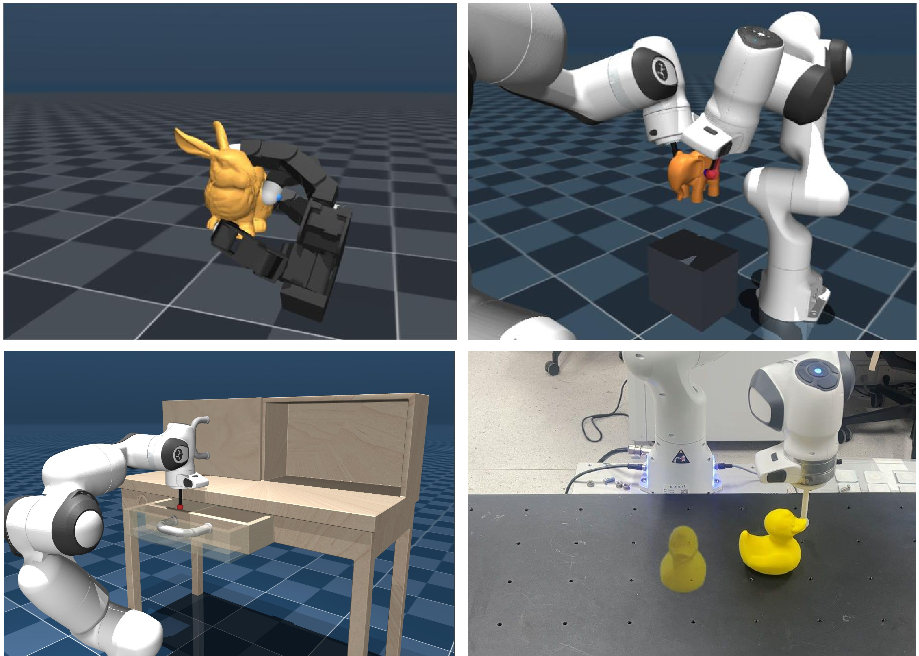
\includegraphics[width=\columnwidth]{figures/scsp_generalization.pdf}}
\caption{\textcolor{red}{
SCSP enables online contact selection and closed-loop generation of diverse manipulation trajectories, allowing it to address a wide range of challenging contact-rich manipulation tasks.
}}
\label{fig:scsp_fig1}
\end{figure}

\begin{table*}[t]
\centering
\caption{Comparison of Contact Planning Methods. \madd{``Generalization'' in this paper refers to cross-task generalization across robot embodiments and task settings; the cross-object generalization reported by DyWA~\cite{lyu2025dywa} is within a trained task.}}
\label{tab:comparison}
\small
\begin{tabularx}{\textwidth}{l c c c c c}
\toprule
\textbf{Methods}
& \textbf{Perception}
& \textcolor{red}{\textbf{Active Contact Selection}}
& \textbf{6D Manip. Exp.}
& \textbf{Real-Time}
& \textcolor{red}{\textbf{No Obj.-Specific Analytic Geom.}} \\
\midrule

C3~\cite{aydinoglu2024consensus}
& \textcolor{red}{Exact State}
& \ding{55}
& \ding{55}
& \ding{51}
& \ding{55} \\

CRISP~\cite{li2025surprising}
& \textcolor{red}{Exact State}
& \textcolor{red}{\ding{55}}
& \ding{55}
& \ding{51}
& \ding{55} \\

IDTO~\cite{kurtz2026inverse}
& \textcolor{red}{Exact State}
& \ding{55}
& \ding{51}
& \ding{51}
& \ding{55} \\

CQDCs~\cite{pang2023global}
& \textcolor{red}{Exact State}
& \ding{55}
& \ding{51}
& \ding{51}
& \ding{55} \\

CF-MPC~\cite{jin2024complementarity}
& \textcolor{red}{Exact State}
& \ding{55}
& \ding{51}
& \ding{51}
& \ding{51} \\

STOCS-3D~\cite{zhang2025simultaneous}
& \textcolor{red}{Exact State}
& \textcolor{red}{\ding{55}}
& \ding{51}
& \ding{55}
& \ding{51} \\

\textcolor{red}{ContactSDF~\cite{yang2024contactsdf}}
& \textcolor{red}{Vision}
& \textcolor{red}{\ding{55}}
& \textcolor{red}{\ding{51}}
& \textcolor{red}{\ding{51}}
& \textcolor{red}{\ding{51}} \\

DyWA~\cite{lyu2025dywa}
& Vision
& \textcolor{red}{\ding{55}}
& \ding{51}
& \ding{51}
& \ding{51} \\

Sampling~\cite{venkatesh2025approximating}
& Vision
& \ding{51}
& \ding{51}
& \ding{51}
& \ding{51} \\

\midrule

\textbf{SCSP}
& Vision
& \ding{51}
& \ding{51}
& \ding{51}
& \ding{51} \\

\bottomrule
\end{tabularx}
\end{table*}

\textcolor{red}{Contact-implicit trajectory optimization (CITO) subsequently avoids this explicit mode decomposition by modeling robot--object interaction (ROI) with complementary contact dynamics and solving the resulting trajectory optimization problem in a unified framework.}
CITO was first applied to locomotion \cite{posa2014direct, wensing2023optimization} and later extended to manipulation.
We mainly focus on Contact-Implicit Model Predictive Control (CIMPC),
\textcolor{red}{
as its receding-horizon formulation continuously replans from the current state and is therefore particularly suitable for real-time closed-loop contact-rich manipulation.
}
\textcolor{red}{CIMPC embeds contact dynamics as constraints in a nonlinear programming (NLP) solver to compute the robot's control inputs online.}
CIMPC incorporates approximated time-stepping contact dynamics \cite{stewart2000implicit, anitescu2006optimization} into trajectory optimization, enabling online hybrid contact planning.
\textcolor{red}{Because contact models commonly used in physical simulators are often formulated as linear complementarity problems (LCPs) or quadratic programs (QPs), directly using them can hinder efficient online optimization. CIMPC methods therefore often adopt approximate contact models that trade physical fidelity for computational efficiency.}
\textcolor{red}{
Representative methods improve the efficiency and scalability of this process through different contact-model approximations and optimization strategies \cite{aydinoglu2024consensus, pang2023global, bui2025push}. In particular, CF-MPC \cite{jin2024complementarity} introduces a complementarity-free contact model to improve the efficiency of online contact-implicit MPC, substantially accelerating contact-rich optimization.
}

\textcolor{red}{
Although CIMPC enables online planning of contact-mode transitions, actively selecting contact locations on the object remains challenging. Contact geometry and complementarity constraints make the resulting optimization nonsmooth and nonconvex, while contact-free states often provide ineffective gradients toward candidate contacts. Because contact locations are typically determined implicitly by the robot trajectory, short planning horizons and local optimization can obscure the long-term benefits of reaching distant contacts. Recent methods improve contact-rich optimization and execution: Suh et al. \cite{suh2025dexterous} introduce a contact-trust-region formulation, Jiang et al. \cite{jiang2025robust} integrate motion--contact planning with tracking, ContactSDF \cite{yang2024contactsdf} provides differentiable multi-contact models, and CRISP \cite{li2025surprising} discovers contact sequences within contact-implicit optimization. These methods, however, do not explicitly select task-relevant robot--object contact locations; CRISP is also evaluated primarily in planar settings. Venkatesh et al. \cite{venkatesh2025approximating} address this issue by sampling contact candidates and solving a local CIMPC problem for each, but at the cost of repeated lower-level optimization. Xie et al. \cite{xie2026touch} use a hierarchical RL--MPC policy to select contacts for a low-level CIMPC controller, but require task-specific training. Efficient task-directed contact selection for closed-loop planning therefore remains unresolved.
}

\textcolor{red}{
In this work, we propose Simultaneous Contact Selection and Planning (SCSP), a cascaded optimization framework for complex contact-rich manipulation. SCSP comprises Contact Selection Optimization (CSO), which performs object-centric search over candidate contact locations and provides contact guidance to steer optimization away from local optima, and Contact Planning Optimization (CPO), which plans robot actions to execute the guided contact while retaining the freedom to realize a nearby feasible contact for flexible execution. A ranking strategy couples the two modules in a cascade by comparing the CSO-guided contact with nearby candidates and passing the resulting reference to CPO.
}

\rev{Table \ref{tab:comparison} summarizes the scope of SCSP relative to representative contact-planning methods. The contributions are:}

\begin{itemize}

 \item
 \textcolor{red}{
 An efficient contact selection method, CSO, is developed for online contact-guidance generation. It samples a candidate point set and performs batched optimization to avoid direct surface-gradient search and the associated nonsmoothness of contact selection. A lightweight surrogate contact model (SCM) enables fast evaluation of candidate utility and selection of the best contact as guidance.
 }

 \item
 \textcolor{red}{
 A contact planning method, CPO, is proposed with a unified cost formulation for generating approach, contact-establishment, and contact-switching trajectories.
 }

 \item
 \textcolor{red}{
 A ranking strategy forms the cascade between contact guidance and planning by ranking the guided contact together with nearby feasible candidates. This preserves task-directed guidance while allowing CPO to select an executable nearby contact, thereby maintaining execution flexibility and contact-trajectory diversity.
 }

 \item
 \textcolor{red}{
 Extensive simulation and real-world experiments validate SCSP across diverse object geometries and contact-rich tasks. Real-world experiments further demonstrate robust vision-based nonprehensile manipulation using only simple contact calibration and without exact object perception.
 }

\end{itemize}

The rest of the paper is organized as follows. Section \ref{sec:preliminaries} reviews the preliminaries. The CSO and CPO are introduced in Sections \ref{sec:cso} and \ref{sec:cpo}, respectively. Section \ref{sec:experiment} presents the experimental results, and
\textcolor{red}{
Section \ref{sec:generalize} evaluates extensions of the SCSP architecture to additional contact-rich manipulation settings.
}
Finally, discussion and limitations are presented in Section \ref{sec:discussion}, and conclusions are drawn in Section \ref{sec:conclusion}.

\section{Preliminaries}
\label{sec:preliminaries}

\textcolor{red}{
We begin with a brief overview of the contact-dynamics and contact-planning formulations used throughout this work.
Section~\ref{preliminaries:contact_dynamics} introduces time-stepping contact dynamics and the associated complementarity formulation.
Section~\ref{preliminaries:contact_planning} introduces model-based contact planning and reviews CIMPC as a representative online formulation.
Section~\ref{preliminaries:complementarity_free} reviews the complementarity-free contact model that motivates the lightweight contact-model approximation used later in CSO.
}

\subsection{Contact Dynamics}
\label{preliminaries:contact_dynamics}

Contact dynamics provides a physical description of interactions among the robot, object, and environment.
Here, we consider the commonly used Anitescu model~\cite{anitescu2006optimization}, which is formulated as the following time-stepping equation:
\begin{subequations}
\label{equ.quasi_dyn}
\begin{align}
 \epsilon\boldsymbol{M}_o\boldsymbol{v}_o
 &=
 h\boldsymbol{\tau}_o
 +
 \sum_{i=1}^{n_c}
 \boldsymbol{J}_{o,i}^{\top}\boldsymbol{\beta}_i,
 \label{equ.quasi_dyn_1}
 \\
 h\boldsymbol{K}_r
 \left(
 h\boldsymbol{v}_r-\boldsymbol{u}
 \right)
 &=
 h\boldsymbol{\tau}_r
 +
 \sum_{i=1}^{n_c}
 \boldsymbol{J}_{r,i}^{\top}\boldsymbol{\beta}_i.
 \label{equ.quasi_dyn_2}
\end{align}
\end{subequations}
\noindent\textcolor{red}{
Here, $\boldsymbol{\beta}_i$ denotes the contact impulse over the time interval $h$.
In the contact-force formulation below, we use $\boldsymbol{\lambda}_i$ to denote the corresponding contact force.
Assuming that the contact force is approximately constant within one time step, they are related by
$\boldsymbol{\beta}_i \approx h\boldsymbol{\lambda}_i$.
}
$\epsilon\boldsymbol{M}_o$, $\boldsymbol{v}_o$, $\boldsymbol{\tau}_o$, and $\boldsymbol{J}_{o,i}$ are the regularized mass matrix, velocity change, non-contact force, and contact Jacobian of the object, respectively.
$\boldsymbol{K}_r$, $\boldsymbol{v}_r$, $\boldsymbol{\tau}_r$, and $\boldsymbol{J}_{r,i}$ are the robot stiffness matrix, velocity, non-contact torque, and contact Jacobian, respectively.


The above equations describe, from the perspective of momentum balance, how the robot influences the object's state through contact, as well as how the object interacts with the environment.
Here, we follow~\cite{pang2021convex,jin2024complementarity} and consider the robot to be under impedance control~\cite{hogan1984impedance}, modeling the robot--object interaction as a spring system.
\textcolor{red}{
The contact constraints between contact forces and system motion are typically formulated as the following cone complementarity problem~\cite{anitescu2010iterative}:
}
\begin{equation}
 \mathcal{K}_i
 \ni
 \boldsymbol{\lambda}_i
 \perp
 \boldsymbol{J}_i\boldsymbol{v}
 +
 \frac{1}{h}
 \begin{bmatrix}
 \phi_i \\
 0 \\
 0
 \end{bmatrix}
 \in
 \mathcal{K}_i^{*},
 \qquad
 \forall i\in\{1,\ldots,n_c\},
 \label{equ.complementarity_constraint}
\end{equation}
\noindent where
 $\mathcal{K}_i
 =
 \left\{
 \boldsymbol{\lambda}_i\in\mathbb{R}^{3}
 \,\middle|\,
 \mu_i\lambda_i^{n}
 \geq
 \left\|\boldsymbol{\lambda}_i^{d}\right\|
 \right\}$
is the Coulomb friction cone, and $\mathcal{K}_i^{*}$ is the dual cone as
 $\mathcal{K}_i^{*}=\left\{
 \boldsymbol{v}
 \,\middle|\,
 \boldsymbol{J}_i^{n}\boldsymbol{v}
 +
 \frac{\phi_i}{h}
 \geq
 \mu_i
 \left\|
 \boldsymbol{J}_i^{d}\boldsymbol{v}
 \right\|
 \right\}$.

The KKT conditions are~\cite{avriel2003nonlinear,anitescu2006optimization}:
\begin{subequations}
\label{equ.contact_model}
\begin{align}
 \min_{\boldsymbol{v}}\quad
 &
 \frac{1}{2}h^{2}
 \boldsymbol{v}^{\top}
 \boldsymbol{Q}
 \boldsymbol{v}
 -
 h
 \boldsymbol{v}^{\top}
 \boldsymbol{b}(\boldsymbol{u}),
 \label{equ.qs_model_obj}
 \\
 \mathrm{s.t.}\quad
 &
 \boldsymbol{J}_i\boldsymbol{v}
 +
 \frac{1}{h}
 \begin{bmatrix}
 \phi_i\\
 0\\
 0
 \end{bmatrix}
 \in
 \mathcal{K}_i^{*},
 \qquad
 i\in\{1,\ldots,n_c\}.
 \label{equ.contact_model_con}
\end{align}
\end{subequations}
\noindent where
$\boldsymbol{Q} \in
\mathbb{R}^{(n_o+n_{\text{DoF}})\times(n_o+n_{\text{DoF}})}$
and
$\boldsymbol{b}(\boldsymbol{u}) \in
\mathbb{R}^{\textcolor{red}{n_o+n_{\text{DoF}}}}$
are
\begin{equation}
 \boldsymbol{Q}
:=
 \begin{bmatrix}
 \epsilon\boldsymbol{M}_o/h^{2} & \boldsymbol{0}\\
 \boldsymbol{0} & \boldsymbol{K}_r
 \end{bmatrix},
 \qquad
 \boldsymbol{b}(\boldsymbol{u})
:=
 \begin{bmatrix}
 \boldsymbol{\tau}_o\\
 \boldsymbol{K}_r\boldsymbol{u}+\boldsymbol{\tau}_r
 \end{bmatrix}.
 \label{equ.q_matrix}
\end{equation}
\noindent Here, $n_o$ and $n_{\mathrm{DoF}}$ are the dimensions of the object and robot states, respectively, and $n_c$ is the number of contacts.

Problem~\eqref{equ.contact_model} is a second-order cone program (SOCP) and is often approximated by a QP through a polyhedral approximation of the friction cone:
\begin{equation}
 \left(
 \boldsymbol{J}_i^{n}
 -
 \mu_i\boldsymbol{J}_{i,j}^{d}
 \right)
 \boldsymbol{v}
 +
 \frac{\phi_i}{h}
 \geq 0,
 \quad
 i\in\{1,\ldots,n_c\},
 \quad
 j\in\{1,\ldots,n_d\},
\end{equation}
\noindent where $n_d$ is the number of friction-cone facets.
Solving~\eqref{equ.contact_model} corresponds to one step of physically consistent contact simulation.
The resulting velocity $\boldsymbol{v}$ can then be used to integrate the current state as
$\boldsymbol{q}_{t+1}
=
\boldsymbol{q}_{t}
\oplus
h\boldsymbol{v}$.
Problem~\eqref{equ.contact_model} and its variants are widely used in physics simulators.

\subsection{Model-based Contact Planning}
\label{preliminaries:contact_planning}

Contact planning refers to generating trajectories for approaching, making contact, and breaking contact with the object to manipulate it to a target state.
Model-based contact planning methods integrate contact dynamics and solve trajectory optimization problems.
As a representative method, CIMPC is formulated as:
\begin{equation}
\begin{aligned}
 \min_{\boldsymbol{u}_{0:N-1}}\quad
 &
 \sum_{k=0}^{N-1}
 \ell(\boldsymbol{x}_k,\boldsymbol{u}_k)
 +
 V_f(\boldsymbol{x}_N)
 \\
 \mathrm{s.t.}\quad
 &
 \boldsymbol{x}_{k+1}
 =
 f(\boldsymbol{x}_k,\boldsymbol{u}_k),
 \quad
 k=0,\ldots,N-1,
 \\
 &
 \boldsymbol{x}_k\in\mathcal{X},
 \quad
 k=0,\ldots,N,
 \\
 &
 \boldsymbol{u}_k\in\mathcal{U},
 \quad
 k=0,\ldots,N-1.
\end{aligned}
\label{eq:CIMPC_opt}
\end{equation}
\noindent in which $\boldsymbol{x}_k$ is the system state, including the object pose $q_k$ and robot configuration, and $f$ denotes the contact dynamics.
The stage cost $\ell$ can take various forms and is typically used to guide the process of approaching the contact location.

\noindent\textcolor{red}{
The hybrid nature of contact dynamics renders~\eqref{eq:CIMPC_opt} a piecewise-smooth nonlinear complementarity problem (NCP).
The full contact model is too costly for online receding-horizon optimization, so we use efficient approximations.
}

\subsection{Complementarity-free Model}
\label{preliminaries:complementarity_free}

\textcolor{red}{
We next introduce the complementarity-free contact model proposed in~\cite{jin2024complementarity}, which motivates the contact-model approximation used later in CSO.
}
Problem~\eqref{equ.contact_model} \textcolor{red}{has the following regularized dual after polyhedral approximation}:
\begin{multline}
\label{equ.dual_prob_relax}
 \max_{\boldsymbol{\beta}\geq\boldsymbol{0}}
 \quad
 -\frac{1}{2h^{2}}
 \boldsymbol{\beta}^{\top}
 \left(
 \boldsymbol{\widetilde{J}}
 \boldsymbol{Q}^{-1}
 \boldsymbol{\widetilde{J}}^{\top}
 +
 \boldsymbol{R}
 \right)
 \boldsymbol{\beta}
 \\
 -
 \frac{1}{h}
 \left(
 \boldsymbol{\widetilde{J}}
 \boldsymbol{Q}^{-1}
 \boldsymbol{b}
 +
 \boldsymbol{\widetilde{\phi}}
 \right)^{\top}
 \boldsymbol{\beta}
 -
 \frac{1}{2}
 \boldsymbol{b}^{\top}
 \boldsymbol{Q}^{-1}
 \boldsymbol{b}.
\end{multline}
\noindent in which $\boldsymbol{R}$ is a small regularization term commonly used to enhance numerical stability, and
\begin{equation}
\boldsymbol{\widetilde{J}}
=
\begin{bmatrix}
 \boldsymbol{J}_1^n-\mu_1\boldsymbol{J}_{1,1}^t\\
 \vdots\\
 \boldsymbol{J}_1^n-\mu_1\boldsymbol{J}_{1,\mathreplace{n_t}{n_d}}^t\\
 \vdots\\
 \boldsymbol{J}_{n_c}^n-\mu_{n_c}\boldsymbol{J}_{n_c,1}^t\\
 \vdots\\
 \boldsymbol{J}_{n_c}^n-\mu_{n_c}\boldsymbol{J}_{n_c,\mathreplace{n_t}{n_d}}^t
\end{bmatrix},
\boldsymbol{\widetilde{\phi}}
=
\begin{bmatrix}
 \phi_1\\
 \vdots\\
 \phi_1\\
 \vdots\\
 \phi_{n_c}\\
 \vdots\\
 \phi_{n_c}
\end{bmatrix},
\boldsymbol{\beta}
=
\begin{bmatrix}
 \beta_{1,1}\\
 \vdots\\
 \beta_{1,n_d}\\
 \vdots\\
 \beta_{n_c,1}\\
 \vdots\\
 \beta_{n_c,n_d}
\end{bmatrix}.
\end{equation}
\noindent\textcolor{red}{Here, $\boldsymbol{\beta}$ contains nonnegative facet impulse coefficients, mapped to generalized impulse by $\boldsymbol{\widetilde{J}}^{\top}$. The directional tangential Jacobians $\boldsymbol{J}_{i,j}^{t}$ correspond to $\boldsymbol{J}_{i,j}^{d}$ above.}
Specifically, the solution of~\eqref{equ.dual_prob_relax} satisfies the following complementarity constraints:
\begin{equation}
\label{equ.dual_prob_relax_sol}
 \boldsymbol{0}
 \leq
 \boldsymbol{\beta}
 \perp
 \frac{1}{h}
 \left(
 \boldsymbol{\widetilde{J}}
 \boldsymbol{Q}^{-1}
 \boldsymbol{\widetilde{J}}^{\top}
 +
 \boldsymbol{R}
 \right)
 \boldsymbol{\beta}
 +
 \left(
 \boldsymbol{\widetilde{J}}
 \boldsymbol{Q}^{-1}
 \boldsymbol{b}
 +
 \boldsymbol{\widetilde{\phi}}
 \right)
 \geq
 \boldsymbol{0}.
\end{equation}
\noindent Following~\cite{jin2024complementarity}, we replace the dense inverse
$(\boldsymbol{\widetilde{J}}\boldsymbol{Q}^{-1}
\boldsymbol{\widetilde{J}}^{\top}+\boldsymbol{R})^{-1}$ by a
positive-definite diagonal matrix $\boldsymbol{K}(\boldsymbol{q})$ chosen
as a local approximation. This replacement defines a modified dual
problem. It is not an equality that holds for a general multi-contact
geometry. With $\boldsymbol{D}=\boldsymbol{K}^{-1}$, the modified
problem has the following closed-form solution:
\begin{equation}
 \boldsymbol{\beta}^{+}
 =
 \max
 \left(
 -h
 \boldsymbol{K}(\boldsymbol{q})
 \left(
 \boldsymbol{\widetilde{J}}
 \boldsymbol{Q}^{-1}
 \boldsymbol{b}
 +
 \boldsymbol{\widetilde{\phi}}
 \right),
 \boldsymbol{0}
 \right).
 \label{eq:cf_impulse}
\end{equation}
\noindent\textcolor{red}{The complementarity-free model is then written as:}
\begin{equation}
\label{equ:cf_model}
f_{\mathrm{cf}}:
\begin{cases}
 \boldsymbol{v}^{+}
 =
 \dfrac{1}{h}
 \boldsymbol{Q}^{-1}
 \boldsymbol{b}
 +
 \dfrac{1}{h\rev{^{2}}}
 \boldsymbol{Q}^{-1}
 \boldsymbol{\widetilde{J}}^{\top}
 \boldsymbol{\beta}^{+},
 \\[2mm]
 \boldsymbol{x}_{k+1}
 =
 \boldsymbol{x}_{k}
 +
 h
 \left(
 \boldsymbol{v}_{k}
 +
 \boldsymbol{v}^{+}
 \right).
\end{cases}
\end{equation}
\noindent where $\boldsymbol{\beta}$ denotes the \textcolor{red}{polyhedral contact-impulse coefficients} and $\boldsymbol{v}^{+}$ combines the object velocity $\boldsymbol{v}_o$ and robot velocity $\boldsymbol{v}_r$.

\begin{figure*}
 \centerline{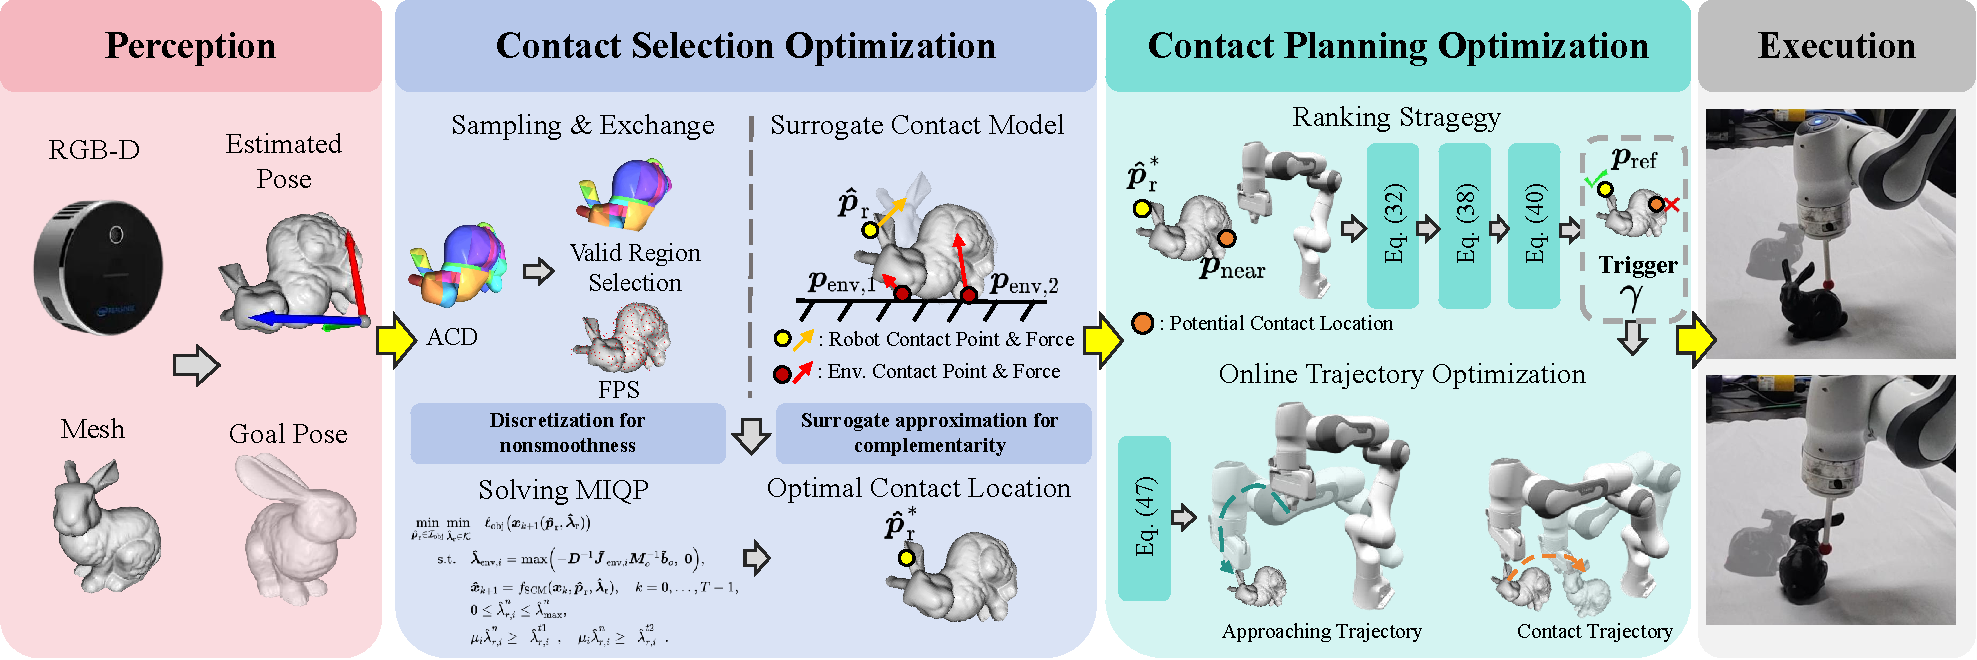
\includegraphics[width=\textwidth]{figures/framework.pdf}}
\caption{Framework structure of SCSP. SCSP consists of Contact Selection Optimization (CSO) and Contact Planning Optimization (CPO). CSO discretizes nonsmooth geometry through the Sampling \& Exchange method and introduces a surrogate contact model for efficient approximation of contact dynamics. CSO online computes the \rev{optimal contact location among candidate contact set} $\boldsymbol{\hat{p}}_{\text{r}}^*$ as contact prior. The ranking strategy in CPO further evaluates whether the nearest point $\boldsymbol{p}_{\text{near}}$ can serve as a feasible suboptimal substitute for $\boldsymbol{\hat{p}}_{\text{r}}^*$ as the reference contact location, after which trajectory optimization is solved online to generate the approach and contact trajectories.}
\label{fig:framework}
\end{figure*}

\section{Contact Selection Optimization}
\label{sec:cso}

In this section, we present the design of CSO.
We begin by analyzing the key challenges of integrating contact selection into CIMPC, which limit the diversity of existing methods.
\textcolor{blue}{
We then formulate the contact selection problem and discuss the main difficulties in solving it.
}
Finally, we present the detailed design of our CSO module for online contact selection.


\subsection{Why Contact Selection is necessary?} 

\textcolor{red}{Contact selection refers to choosing object contact locations $\left \{ \boldsymbol{p}_{\mathcal{O}, i} \right \} \subset \partial \mathcal{O}$ that can generate task-beneficial wrenches for changing the object pose. According to \eqref{equ.quasi_dyn_1} and \eqref{equ.quasi_dyn_2}, the object wrench is jointly determined by the contact Jacobian, which depends on the contact location and its local geometry, and the contact impulse $\boldsymbol{\beta}_i$ (or, equivalently, the contact force $\boldsymbol{\lambda}_i$). For some contact locations, no force within the corresponding friction cone can produce a wrench that improves the object pose; contact switching is therefore necessary.}

\textcolor{red}{CIMPC models robot--object interaction (ROI) with contact dynamics whose informative gradients are confined to the low-dimensional contact manifold $\mathcal{S}_{\text{contact}}$ embedded in the full state space $\mathcal{S}$. The contact-free manifold $\mathcal{S}_{\text{free}}$ provides no effective contact-induced gradient, making autonomous contact selection difficult and requiring attractive costs or reference trajectories to induce contact. Although CIMPC can choose between contact and non-contact modes, its short receding horizon may not reveal, within the fixed horizon, the benefit of reaching a distant contact location.}

Rather than integrating contact selection into the CIMPC formulation, we study how to formulate contact selection as a separate optimization problem. As illustrated in Fig. \ref{fig:framework}, we first simplify the problem by ignoring the planning of the robot contact locations $\left \{ \boldsymbol{p}_{\mathcal{R}, i} \right \}$ and thereby obtain the following object-centric optimization problem:
\begin{equation}
    \begin{aligned}
        \min_{\boldsymbol{p}_{\text{r}} \in \partial \mathcal{O}, \boldsymbol{\lambda} \in \mathcal{K}} & 
        \ell_{\text{cso}}(\boldsymbol{x}_{\textcolor{red}{T}}) \\
        \text{s.t.} \quad 
        & \boldsymbol{x}_{k+1} = f(\boldsymbol{x}_k, \boldsymbol{p}_{\text{r}}, \boldsymbol{\lambda}),
        \quad k = 0, \dots, T-1.
    \end{aligned}\label{scsp}
\end{equation}
where $\mathcal{K}$ is the set of feasible contact forces and $\ell_{\text{cso}}(\cdot)$ is the objective of contact selection. $\boldsymbol{p}_{\text{r}} \in \mathbb{R}^{3 \times n_{\text{r}}}$ represents the locations where the robot applies contacts to the object, with $n_{\text{r}}$ denotes the number of robot contacts. \eqref{scsp} addresses the gradient sparsity issue arising from hybrid planning in the original contact-rich manipulation problem by defining CSO to solve for \rev{low-cost sampled contact locations} and contact forces on $\mathcal{S}_{\text{contact}}$. The neglected process of the robot approaching $\mathcal{S}_{\text{contact}}$ from its current state is the primary source of the gradient sparsity. Note that \eqref{scsp} is hard to solve due to the coupling of contact location $\boldsymbol{p}_{\text{r}}$ and the contact force $\boldsymbol{\lambda}=\left [ \boldsymbol{\lambda}_{\text{env}}, \boldsymbol{\lambda}_{\text{r}} \right ]$. Therefore, we adopt a commonly used simplification for handling nonconvex optimization problems to reformulate (\ref{scsp}) as subproblems:
\begin{equation}
    \min_{\boldsymbol{p}_{\text{r}} \in \partial \mathcal{O}}
    \quad V(\boldsymbol{p}_{\text{r}})\label{equ:outer_loop},
\end{equation}
in which:
\begin{equation}
\begin{aligned}
V(\boldsymbol{p}_{\text{r}})
:= \min_{\boldsymbol{\lambda}_{\text{r}} \in \mathcal{K}} \quad &
\ell_{\text{cso}}(\boldsymbol{x}_{\textcolor{red}{T}}) \\
\text{s.t.} \quad
& \boldsymbol{x}_{k+1}
= f(\boldsymbol{x}_k, \boldsymbol{p}_{\text{r}}, \boldsymbol{\lambda}_{\text{r}}, \boldsymbol{\lambda}_{\text{env}}),
\quad k = 0, \dots, T-1.
\end{aligned}\label{equ:inner_loop}
\end{equation}
The physical interpretation of \eqref{equ:outer_loop} and \eqref{equ:inner_loop} is that a contact location is regarded as optimal if applying the best possible combination of contact force $\boldsymbol{\lambda}^*$ yields the minimum motion cost of the object. Despite the simplifications, \eqref{equ:outer_loop} remains a complex problem with nonsmooth constraints $\boldsymbol{p}_{\text{r}} \in \partial \mathcal{O}$ that depend on the object geometry. Meanwhile, \eqref{equ:inner_loop} is a complementary problem with coupled environment forces $\boldsymbol{\lambda}_{\text{env}}$ and robot contact forces $\boldsymbol{\lambda}_{\text{r}}$. The nonconvexity makes online CSO intractable. We next present the solutions to further simplify both \eqref{equ:outer_loop} and \eqref{equ:inner_loop} to improve computational efficiency. 



\subsection{Sampling and Exchange Method}\label{sec:sampling&exchange}
The nonsmoothness on the object geometry leads to discontinuities in the gradient of \eqref{equ:outer_loop}. The inherently nonsmooth nature of the problem motivates us to adopt a sampling-based method. To simplify \eqref{equ:outer_loop}, we uniformly sample a set of candidate contact point set $\mathcal{I}_{\text{obj}} = \{\boldsymbol{p}_i\}_{i=1}^{n_s}$ on the object surface $\partial \mathcal{O}$, thus reformulate \eqref{equ:outer_loop} as:
\begin{equation}
    \min_{\boldsymbol{p}_{\text{r}} \in \mathcal{I}_{\text{obj}}}
    \quad V(\boldsymbol{p}_{\text{r}}),\label{equ:simplify_outer_loop}
\end{equation}
When the sampling is sufficiently uniform, \eqref{equ:simplify_outer_loop} provides a good approximation to \eqref{equ:outer_loop} and is not affected by discontinuous gradients caused by the geometry. To obtain a high quality candidate set, $\mathcal{I}_{\text{obj}}$ should satisfy the following conditions:
\begin{itemize}
    \item \textbf{Physical reachability}, which requires that candidate contact locations be reachable by the robot, i.e., within the robot workspace and not occluded.
    \item \textbf{Contact stability}, which requires avoiding regions with high curvature where stable contact is difficult to apply.
    \item \textbf{Uniform distribution}, which means the sampled points are representative of approximating the original geometry.
\end{itemize}
These conditions require the sampling method to maintain uniform coverage while prioritizing manipulability over local geometric details. To address this, we propose an efficient sampling strategy as shown in Algorithm \ref{algorithm:sampling}. We first perform approximate convex decomposition (ACD) \cite{lien2007approximate} to obtain a convex approximation $\mathcal{F}$ of the original geometry $\mathcal{O}$. ACD decomposes the object into convex polygons, mitigating interference caused by local geometric details and reducing computational cost. Moreover, these polygons are typically larger and flatter, which implies greater contact stability and improved reachability.

Then we perform Farthest-Point Sampling (FPS) on the convex approximation to uniformly sample points on the polygons. Starting from an arbitrary point as a sample, the algorithm iteratively selects the points that maximize the minimal Euclidean distance to all previously chosen samples:
\begin{equation}
p'_{k+1} = \arg\max_{p_i \in \mathcal{F}} \min_{p'_j \in \mathcal{I}_{k}} \|\boldsymbol{p}_i - \boldsymbol{p}'_j\|^2, \label{equ:FPS}
\end{equation}
where $\mathcal{I}_{k}$ is the set of already selected samples. The sampling process is performed offline. Solving \eqref{equ:FPS} yields a uniformly distributed set of points $\mathcal{I}_{\text{obj}}$. For each sampled point $p'_j \in \mathcal{I}_{k}$, we also construct its local coordinate frame to obtain the tangential and normal vectors as local contact information. The local orthonormal frame is constructed as $(\boldsymbol{n}_i, \boldsymbol{t}_{1,i}, \boldsymbol{t}_{2,i})$ in which the normal vector $\boldsymbol{n}_i$ is obtained from the mesh or point-cloud normal estimate, and two orthogonal tangent directions are computed as:
\begin{equation}
\boldsymbol{t}_{1,i} = 
\frac{\boldsymbol{a} - (\boldsymbol{a} \cdot \boldsymbol{n}_i)\boldsymbol{n}_i}
{\|\boldsymbol{a} - (\boldsymbol{a} \cdot \boldsymbol{n}_i)\boldsymbol{n}_i\|}, \ 
\boldsymbol{t}_{2,i} = \boldsymbol{n}_i \times \boldsymbol{t}_{1,i},
\end{equation}
where $\boldsymbol{a}$ is an arbitrary fixed axis. \textcolor{red}{When the reference axis $a$ is nearly parallel to the surface normal $n_i$, we select another coordinate axis as the reference axis to avoid numerical singularity.} We use this local geometric information to compute the Jacobian required for contact force optimization. Furthermore, a KD-tree $\mathcal{T}=\left \{ (\boldsymbol{p}_i,\boldsymbol{n}_i, \boldsymbol{t}_{1,i}, \boldsymbol{t}_{2,i}) \right \}^{n_s}_{i=1} $ is constructed over the set $\mathcal{I}_{\text{obj}}$ to enable efficient nearest-neighbor queries.

An online Valid Region Selection procedure is further applied to identify feasible and task-relevant surface regions, filtering out unreachable or low-quality points such as occluded regions, regions outside the robot workspace, and \rev{regions that violate task-specific semantic masks (for example, handles or forbidden surfaces).} The valid region is maintained by applying a mask to $\mathcal{F}$ to obtain $\mathcal{F}_{\text{v}}$, and then selecting points on $\mathcal{F}_{\text{v}}$ to obtain $\mathcal{I}_{\text{avail}}$. To better illustrate the process, consider the toy example shown in Fig. \ref{fig:FPS}. First, following the procedure illustrated in Fig. \ref{fig:FPS}(a), we iteratively apply \eqref{equ:FPS} to obtain a set of uniformly distributed sampling points over the processed object mesh. We then partition the surface online into a set of valid regions and masked regions, and select the points that lie within the valid regions to form the candidate set $\mathcal{I}_{\text{avail}}$, as shown in Fig. \ref{fig:FPS}(b).

\begin{figure}[!t]
 \centerline{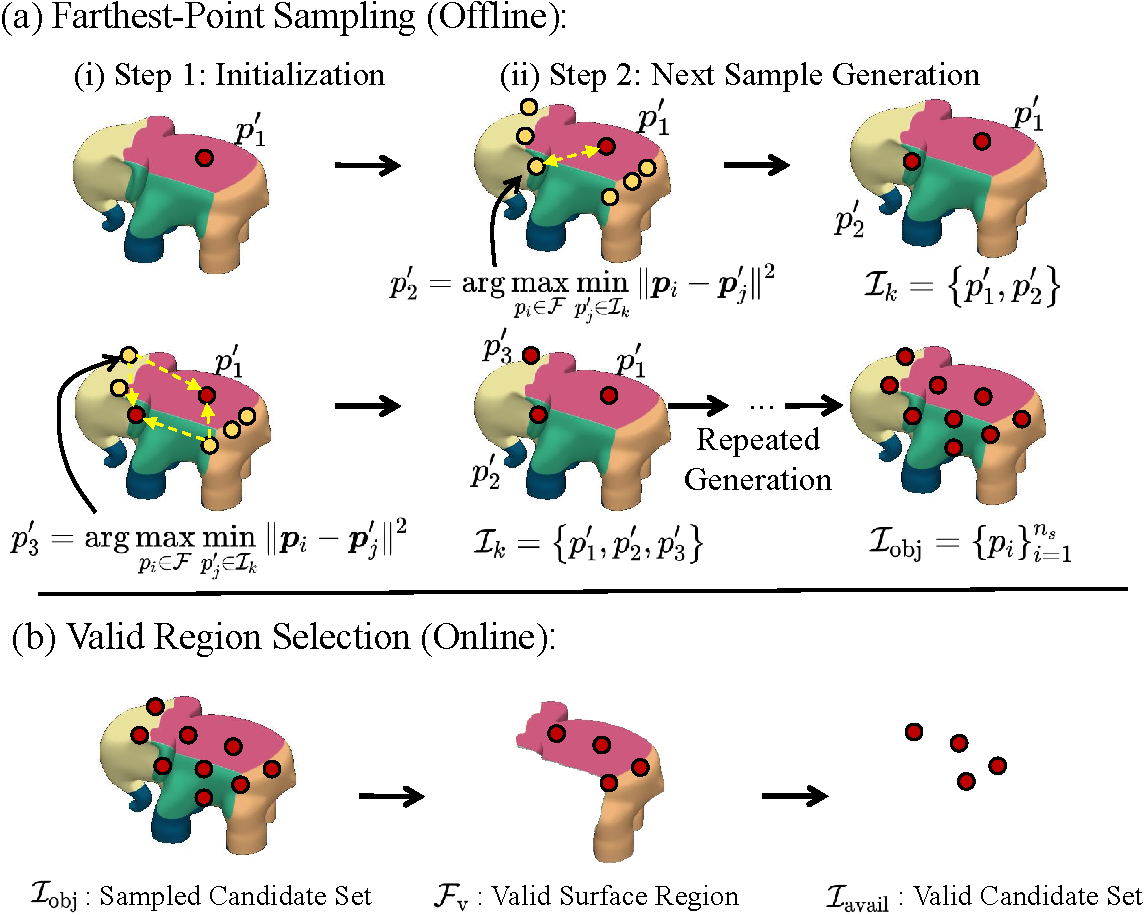
\includegraphics[width=\columnwidth]{figures/sampling_strategy.pdf}}
\caption{The sampling strategy in CSO. The candidate point set is sampled sequentially through: (a) Farthest-Point Sampling to uniformly sample points on the object, and (b) Valid Region Selection to select valid points for contact.}
\label{fig:FPS}
\end{figure}

\begin{algorithm}[t]
\caption{Sampling and Exchange Method}
\label{algorithm:sampling}
\begin{algorithmic}[1]
\Require Object geometry $\mathcal{O}$, sample count $K$, fixed axis $\boldsymbol{a}$
\Ensure $\mathcal{T}= \left \{ (\boldsymbol{p}_i,\boldsymbol{n}_i, \boldsymbol{t}_{1,i}, \boldsymbol{t}_{2,i}) \right \}^{n_s}_{i=1}$ and $\mathcal{I}_{\text{avail}}$.

\State $\mathcal{F} \gets \text{ACD}(\mathcal{O})$ \Comment{Convex approximation}
\State Initialize $\mathcal{I}_{k} \gets \{p'_1\}$ with an arbitrary seed in $\mathcal{F}$
\For{$k=1$ to $K-1$}
    \State $p'_{k+1} \gets \arg\max_{p'_i\in \mathcal{F}} \min_{p_j\in \mathcal{I}_{k}} \|\boldsymbol{p}'_i-\boldsymbol{p}'_j\|^2$
    \State $\mathcal{I}_{\text{obj}} \gets \mathcal{I}_{k} \cup \{p'_{k+1}\}$ \Comment{Obtain candidate set $\mathcal{I}_{\text{obj}}$}
\EndFor
\State $\mathcal{F}_{\text{v}} \gets \text{getValidRegion}(\mathcal{F})$ \Comment{Task-specific segment}
\ForAll{$p_i \in \mathcal{I}_{\text{obj}}$}
    \If{$p_i \notin \mathcal{F}_{\text{v}}$}
        \State Remove $p_i$ from $\mathcal{I}_{\text{obj}}$ \Comment{Valid region selection}
        \State \textbf{continue}
    \EndIf \Comment{Obtain $\mathcal{I}_{\text{avail}}$}
    \State Estimate normal $\boldsymbol{n}_i$ from $\mathcal{F}$ at $p_i$
    \State $\boldsymbol{t}_{1,i} \gets \dfrac{\boldsymbol{a}-(\boldsymbol{a}\cdot\boldsymbol{n}_i)\boldsymbol{n}_i}{\|\boldsymbol{a}-(\boldsymbol{a}\cdot\boldsymbol{n}_i)\boldsymbol{n}_i\|}$, \ $\boldsymbol{t}_{2,i} \gets \boldsymbol{n}_i \times \boldsymbol{t}_{1,i}$
\EndFor
\State \Return $\mathcal{T}=\left \{ (\boldsymbol{p}_i,\boldsymbol{n}_i, \boldsymbol{t}_{1,i}, \boldsymbol{t}_{2,i}) \right \}^{n_s}_{i=1}$
\end{algorithmic}
\end{algorithm}

\subsection{Surrogate Contact Model}

The sampling strategy transforms the original optimization into a discrete–continuous optimization problem. We further simplify \eqref{equ:inner_loop} to improve efficiency. Most existing contact models are computationally expensive for scenarios that require repeatedly solving \eqref{equ:inner_loop}. Moreover, the complementarity in contact dynamics and the coupling between $\boldsymbol{\lambda}_{\text{env}}$ and $\boldsymbol{\lambda}_{\text{r}}$  make the optimization difficult to converge, leading to physically inconsistent results. To address this issue and enable online contact selection, we present a surrogate contact model (SCM) as a local approximation of the original contact dynamics. The procedure of SCM is illustrated in Fig. \ref{fig:stick1}. The approximation relies on the following assumptions of the object-environment contact:

\begin{assumption}[Fixed Contact Set]
 The object--environment contact location remains unchanged in each SCM rollout, i.e., no new contacts are created and existing contacts remain.\label{assumption:mode}
\end{assumption}

\begin{assumption}[Multi-Contact Decoupling]
 The contact between the object and the environment can be approximated by independent spring–damper systems, neglecting higher-order dynamic couplings between different contact locations. \label{assumption:decoupling}
\end{assumption}

We reformulate the original contact dynamics in (\ref{equ.quasi_dyn_1}) as:
\begin{equation}
    \epsilon\boldsymbol{M}_o\boldsymbol{v}_o =
    h(\boldsymbol{\tau}_o+\sum\nolimits_{i=1}^{n_{\text{r}}}{\boldsymbol{J}}_{\text{r},i}^{\top}\boldsymbol{\lambda}_{\text{r},i} + \sum\nolimits_{j=1}^{n_{\text{env}}}{\boldsymbol{J}}_{\text{env},j}^{\top}\boldsymbol{\lambda}_{\text{env},j}),
    \label{eq:simplified}
\end{equation}
and we denote $\boldsymbol{\tilde{b}}_o = h(\boldsymbol{\tau}_o+\sum\nolimits_{i=1}^{n_{\text{r}}}{\boldsymbol{J}}_{\text{r},i}^{\top}\boldsymbol{\lambda}_{\text{r},i})$. Similar to (\ref{equ.dual_prob_relax}), the physically consistent environment contact force can be obtained by solving the following dual problem:
\begin{multline}
\max_{\boldsymbol{\lambda}_{\text{env}}\geq \boldsymbol{0}}\quad
    -\frac{1}{2} \boldsymbol{\lambda}_{\text{env}}^\top
    \left(
    \boldsymbol{\tilde{J}}_{\text{env}} \boldsymbol{M}_o^{-1} \boldsymbol{\tilde{J}}_{\text{env}}^\top
    +\boldsymbol{R}
    \right)
    \boldsymbol{\lambda}_{\text{env}} \\
    -
    (\boldsymbol{\tilde{J}}_{\text{env}} \boldsymbol{M}_o^{-1}\boldsymbol{\tilde{b}}_o+\boldsymbol{\tilde{\phi}})^\top
    \boldsymbol{\lambda}_{\text{env}}
    -\frac{1}{2}
    \boldsymbol{\tilde{b}}_o^\top
    \boldsymbol{M}_o^{-1}
    \boldsymbol{\tilde{b}}_o,
    \label{eq:dual_problem}
\end{multline}
and the solution satisfies the complementarity condition
\begin{equation}
\boldsymbol{0}\leq \boldsymbol{\lambda}_{\text{env}} \perp
\boldsymbol{W}_{\text{env}}
\boldsymbol{\lambda}_{\text{env}}
+\boldsymbol{g}_{\text{env}}
\geq \boldsymbol{0}.
\label{eq:env_complementarity}
\end{equation}
where
\begin{equation}
    \boldsymbol{W}_{\text{env}}=\left(
\boldsymbol{\tilde{J}}_{\text{env}} \boldsymbol{M}_o^{-1} \boldsymbol{\tilde{J}}_{\text{env}}^\top
+\boldsymbol{R}
\right), \ \boldsymbol{g}_{\text{env}}=\left(
\boldsymbol{\tilde{J}}_{\text{env}} \boldsymbol{M}_o^{-1}\boldsymbol{\tilde{b}}_o
+\boldsymbol{\tilde{\phi}}
\right).
\end{equation}
Here $\boldsymbol{W}_{\text{env}}$ is the Delassus matrix associated with object–environment contact. Since the contact force at each contact point is decomposed into one normal and two tangential components $
\boldsymbol{\lambda}_i =
[\lambda_i^{n}, \lambda_i^{t_1}, \lambda_i^{t_2}]^\top \in \mathbb{R}^{3}
$, the Delassus matrix $\boldsymbol{W}_{\text{env}}$ admits a block structure
\begin{equation*}
    \boldsymbol{W}_{\text{env}} =
\begin{bmatrix}
\boldsymbol{W}_{11} & \boldsymbol{W}_{12} & \cdots & \boldsymbol{W}_{1n_{\text{env}}} \\
\boldsymbol{W}_{21} & \boldsymbol{W}_{22} & \cdots & \boldsymbol{W}_{2n_{\text{env}}} \\
\vdots & \vdots & \ddots & \vdots \\
\boldsymbol{W}_{n_{\text{env}}1} & \boldsymbol{W}_{n_{\text{env}}2} & \cdots & \boldsymbol{W}_{n_{\text{env}} n_{\text{env}}}
\end{bmatrix},
\end{equation*}
where each block $\boldsymbol{W}_{ij} \in \mathbb{R}^{3\times3}$ is
\begin{equation*}
\boldsymbol{W}_{ij}
=
\begin{bmatrix}
\boldsymbol{J}_i^{n} \\
\boldsymbol{J}_i^{t_1} \\
\boldsymbol{J}_i^{t_2}
\end{bmatrix}
\boldsymbol{M}_o^{-1}
\begin{bmatrix}
(\boldsymbol{J}_j^{n})^\top &
(\boldsymbol{J}_j^{t_1})^\top &
(\boldsymbol{J}_j^{t_2})^\top
\end{bmatrix}
+
\boldsymbol{R}_{ij}.
\end{equation*}
The diagonal blocks $\boldsymbol{W}_{ii}$ describe the local effective inertia at each contact, indicating how forces applied at contact $i$ affect motion along its own constraint directions. The off-diagonal blocks $\boldsymbol{W}_{ij}$ ($i \neq j$) represent dynamic coupling between different contacts. Under Assumption \ref{assumption:decoupling}, these inter-contact couplings are negligible. Therefore, $\boldsymbol{W}_{\text{env}}$ can be approximated by a block-diagonal matrix:
\begin{equation}
\boldsymbol{W}_{\text{env}} = \text{blockdiag}(\boldsymbol{W}_{11}, \boldsymbol{W}_{22}, \ldots, \boldsymbol{W}_{n_{\text{env}} n_{\text{env}}}),
\end{equation}
and \eqref{eq:env_complementarity} is decomposed to subproblems:
\begin{equation}
\boldsymbol{0} \leq \boldsymbol{\lambda}_{\text{env},i} \perp \boldsymbol{W}_{ii} \boldsymbol{\lambda}_{\text{env},i} + (\boldsymbol{\tilde{J}}_{\text{env},i} \boldsymbol{M}_o^{-1}\boldsymbol{\tilde{b}}_o + \boldsymbol{\tilde{\phi}}_i) \geq \boldsymbol{0}.
\label{equ:contact_i_complementarity}
\end{equation}
Furthermore, if $\boldsymbol{W}_{ii}$ admits the low-rank decomposition:
\begin{equation}
\boldsymbol{W}_{ii} = \boldsymbol{D} + \boldsymbol{E}, \label{equ:decomposation}
\end{equation}
where $\boldsymbol{D}$ is a diagonal matrix and
$\boldsymbol{E}$ is relatively small, \eqref{equ:contact_i_complementarity} has the approximated closed-form solution:
\begin{equation}
\boldsymbol{\hat{\lambda}}_{\text{env}, i}
=
\max
\left(
-
\boldsymbol{D}^{-1}
(\boldsymbol{\tilde{J}}_{\text{env},i} \boldsymbol{M}_o^{-1}\boldsymbol{\tilde{b}}_o + \boldsymbol{\tilde{\phi}}_i),
\;\boldsymbol{0}
\right).
\label{eq:quasi-closed_form_solution_nonsmooth}
\end{equation}
With \eqref{eq:quasi-closed_form_solution_nonsmooth}, we can obtain the following lemma:
\begin{lemma}
Under Assumption \ref{assumption:decoupling}, the environment contact force $\boldsymbol{\lambda}_{\text{env}}$ is an explicit function of $\boldsymbol{\lambda}_{\text{r}}$.
\end{lemma}
To obtain a high-quality approximation, we decompose $\boldsymbol{W}_{ii}$ in \eqref{equ:decomposation} as:
\begin{equation}\label{equ:max_decomposition}
\boldsymbol{D} = \operatorname{diag}(\boldsymbol{W}_{ii}) + \epsilon \boldsymbol{I},
\end{equation}
where $\epsilon$ is a small regularization coefficient to ensure numerical stability. \eqref{equ:max_decomposition} gives the closest diagonal approximation to $\boldsymbol{W}_{ii}$ in the Frobenius norm\footnote{Proof see Appendix \ref{proof:closest_approximation}.}. However, it should be noted that \eqref{eq:quasi-closed_form_solution_nonsmooth} is incompatible with gradient-based solvers. When the contact set changes within the CSO horizon, variations in $\boldsymbol{\tilde{J}}_{\text{env},i}$ and $\boldsymbol{\tilde{\phi}}_i$ introduce additional non-smoothness. To address this, we leverage Assumption \ref{assumption:mode} to further derive:
\begin{lemma}\label{lemma2:piecewise-linear}
The environment contact force $\boldsymbol{\lambda}_{\text{env}}$ is a piecewise linear function of $\boldsymbol{\lambda}_{\text{r}}$:
\begin{equation}
\boldsymbol{\hat{\lambda}}_{\text{env}, i}
=
\max
\left(
-
\boldsymbol{D}^{-1}
\boldsymbol{\tilde{J}}_{\text{env},i} \boldsymbol{M}_o^{-1}(\boldsymbol{\tau}_o+\sum\nolimits_{i=1}^{n_{\text{r}}}{\boldsymbol{J}}_{\text{r},i}^{\top}\boldsymbol{\hat{\lambda}}_{\text{r},i}),
\;\boldsymbol{0}
\right).
\label{eq:quasi-closed_form_solution}
\end{equation}
\end{lemma}
\begin{proof}
    \renewcommand{\qedsymbol}{}
    Based on Assumption 1, we can obtain that $\phi \equiv 0$, leading to \eqref{eq:quasi-closed_form_solution}. Moreover, since the contact geometry set remains invariant over the time interval, $\boldsymbol{\tilde{J}}_{\text{env},i}$ is a constant matrix, thus $\boldsymbol{W}_{ii}$ is constant, and $\boldsymbol{D}$, $\boldsymbol{M}_o^{-1}$ are all constant matrices. Therefore, \eqref{eq:quasi-closed_form_solution} is piecewise linear.
\end{proof}
Substituting \eqref{eq:quasi-closed_form_solution} into \eqref{eq:simplified}, we obtain a lightweight model:
\begin{equation}
    f_{\text{SCM}}:\begin{cases}
    \boldsymbol{\hat{v}}^+ =
\frac{1}{h}\boldsymbol{M}_o^{-1}\boldsymbol{\tilde{b}}_o
+
\frac{1}{h}\boldsymbol{M}_o^{-1}\sum_{i=1}^{n_\text{env}} \boldsymbol{\tilde{J}}_{\text{env},i}^\top
\boldsymbol{\hat{\lambda}}_{\text{env},i},
     \\
    \boldsymbol{\hat{x}}_{k+1}=
    \boldsymbol{x}_{k}
    +
    h(\boldsymbol{v}_{k}+\boldsymbol{\hat{v}}^+).
\end{cases} \label{equ:scm}
\end{equation}

\textcolor{red}{To compensate for the inter-contact coupling neglected by the diagonal approximation, SCM applies a single global projection to the environment impulse at each prediction step. Using the current free velocity, define}
\begin{equation}
\textcolor{red}{
\begin{aligned}
\boldsymbol{g}^{\mathrm{step}}_{\mathrm{env}}
&=\boldsymbol{\tilde{J}}_{\mathrm{env}}\boldsymbol{v}_{\mathrm{free}}
  +\boldsymbol{\tilde{\phi}}_{\mathrm{env}}/h,\qquad
\boldsymbol{\beta}^{(0)}_{\mathrm{env}}
=\max\!\left(-\boldsymbol{D}^{-1}\boldsymbol{g}^{\mathrm{step}}_{\mathrm{env}},\boldsymbol{0}\right),\\
\alpha
&=\operatorname{clip}\!\left(
-\frac{(\boldsymbol{g}^{\mathrm{step}}_{\mathrm{env}})^\top
      \boldsymbol{\beta}^{(0)}_{\mathrm{env}}}
     {(\boldsymbol{\beta}^{(0)}_{\mathrm{env}})^\top
      \boldsymbol{W}_{\mathrm{env}}\boldsymbol{\beta}^{(0)}_{\mathrm{env}}},0,1\right),\\
\hat{\boldsymbol{\beta}}_{\mathrm{env}}
&=\alpha\boldsymbol{\beta}^{(0)}_{\mathrm{env}},\qquad
\boldsymbol{s}=\alpha\boldsymbol{g}^{\mathrm{step}}_{\mathrm{env}},\qquad
\hat{\boldsymbol{\beta}}_{\mathrm{env}}
=\max\!\left(-\boldsymbol{D}^{-1}\boldsymbol{s},\boldsymbol{0}\right).
\end{aligned}}
\label{eq:scm_single_step_projection}
\end{equation}
\textcolor{red}{The coefficient $\alpha$ is shared by all environment contacts and is set to one when $\boldsymbol{\beta}^{(0)}_{\mathrm{env}}=\boldsymbol{0}$. The environment impulse in \eqref{equ:scm} is replaced by $\hat{\boldsymbol{\beta}}_{\mathrm{env}}$, with the factors $1/h$ converting impulse to force units. We use $r=10^{-8}$ and evaluate the denominator as $\boldsymbol{z}^{\top}\boldsymbol{M}_o^{-1}\boldsymbol{z}+r\|\boldsymbol{\beta}^{(0)}_{\mathrm{env}}\|_2^2$, where $\boldsymbol{z}=\boldsymbol{\tilde{J}}_{\mathrm{env}}^{\top}\boldsymbol{\beta}^{(0)}_{\mathrm{env}}$, without forming or inverting the full Delassus matrix. The projection is evaluated once per prediction step and does not introduce an additional inner iteration. Away from activation, clipping, and zero-impulse boundaries, the resulting map is piecewise rational.}

This Surrogate Contact Model converts the original contact dynamics into a computationally efficient formulation, enabling \eqref{equ:inner_loop} to be solved using gradient-based solvers.

\begin{figure}[!t]
 \centerline{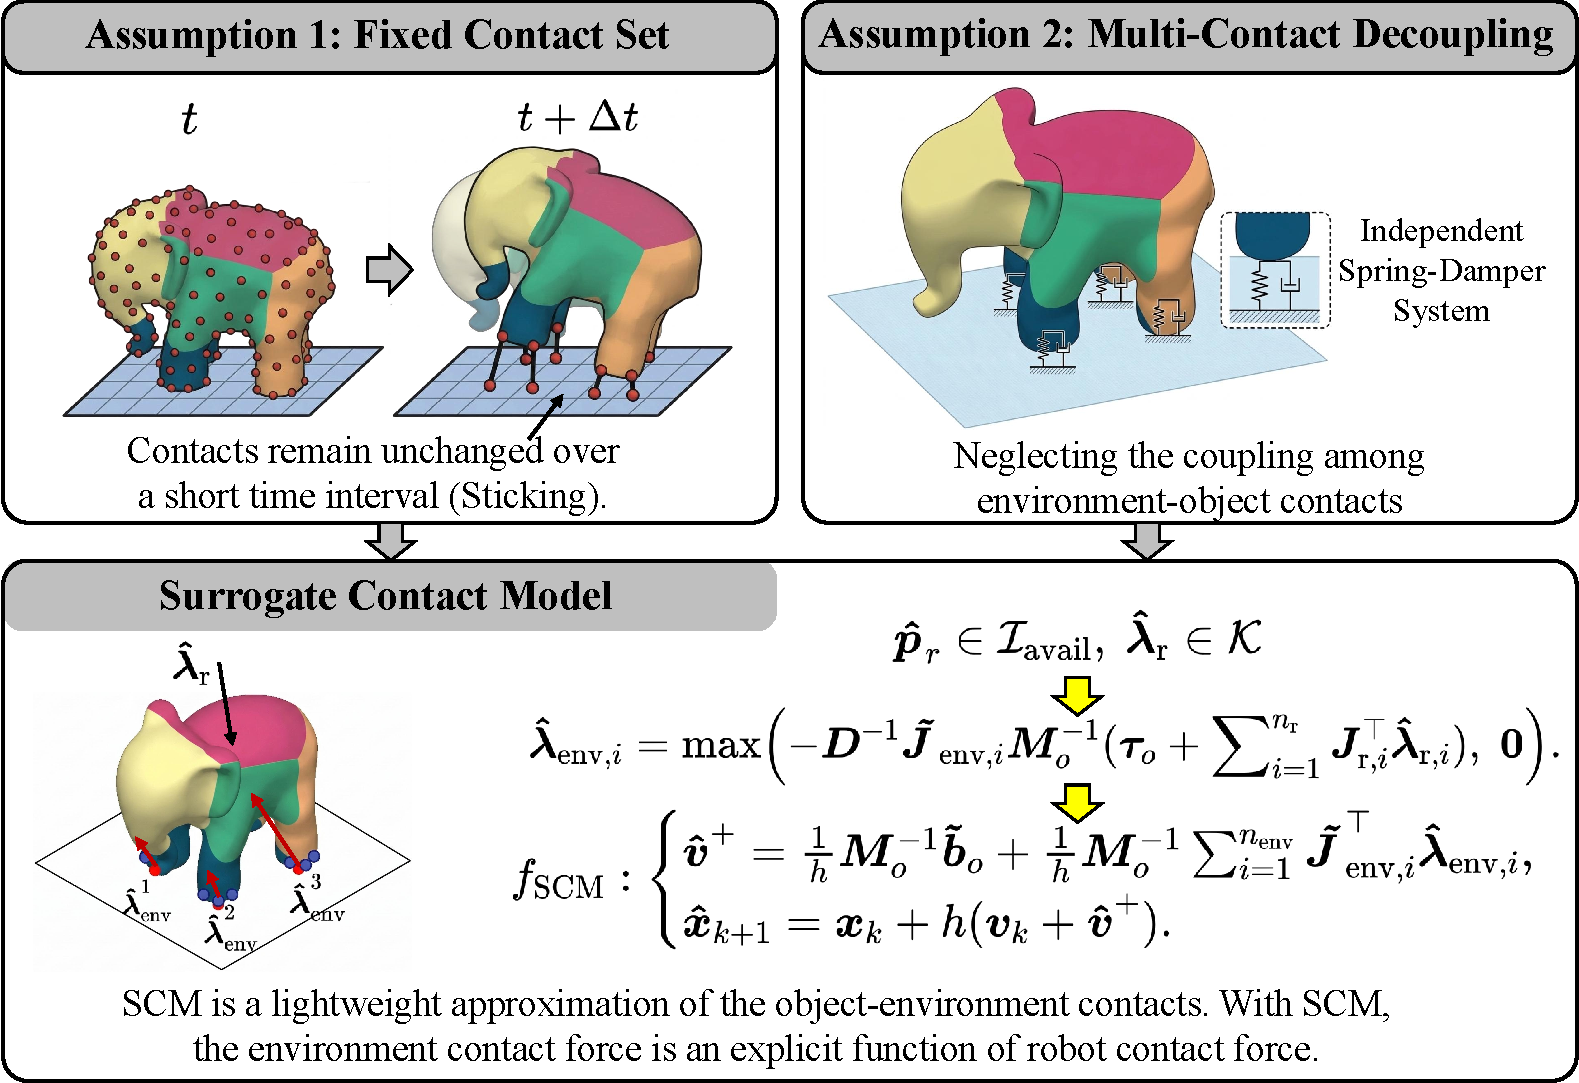
\includegraphics[width=\columnwidth]{figures/surrogate_contact_model.pdf}}
\caption{Illustration of SCM. SCM is a lightweight approximation of the object-environment contact, enabling fast contact selection optimization.}
\label{fig:stick1}
\end{figure}
\subsection{Formulation of CSO}\label{sec:cs_opt}

Integrating SCM into \eqref{equ:inner_loop}, we can obtain the formulation of CSO as: 
\begin{equation} 
\begin{aligned} 
\min_{\boldsymbol{\hat{p}}_{\text{r}} \in \mathcal{I}_{\text{avail}}}\min_{\boldsymbol{\hat{\lambda}}_{\text{r}} \in \mathcal{K}} & \quad 
\ell_{\text{cso}}\big(\boldsymbol{x}_{\textcolor{red}{T}}\big) \\ 
\text{s.t.} \quad
& \hat{\boldsymbol{\beta}}_{\mathrm{env},i}
=\max\!\left(-\boldsymbol{D}^{-1}\boldsymbol{s}_i,\boldsymbol{0}\right),\\
& \boldsymbol{\hat{x}}_{k+1} 
= f_{\text{SCM}}(\boldsymbol{x}_k, \boldsymbol{\hat{p}}_{\text{r}}, \boldsymbol{\hat{\lambda}}_{\text{r}}), 
\quad k = 0, \dots, T-1, \\
& \textcolor{red}{|\hat{\lambda}_{r,i}^{t1}|\leq\mu_i\hat{\lambda}_{r,i}^{n}  , \ |\hat{\lambda}_{r,i}^{t2}|\leq\mu_i\hat{\lambda}_{r,i}^{n}}, \\
& 0 \le \hat{\lambda}^n_{r,i} \le \hat{\lambda}^n_{\text{max}}, \quad i = 0, \dots, n_{\text{r}}.
\end{aligned}\label{equ:csqp} 
\end{equation} 
Here $\boldsymbol{s}_i$ is the contact-$i$ block of $\boldsymbol{s}$ defined in \eqref{eq:scm_single_step_projection}. By solving this discrete-continuous optimization problem, we can obtain the \rev{optimal contact location among candidate contact set $\boldsymbol{\hat{p}}_r^* \in \mathcal{I}_{\text{avail}}$} as guidance for the lower-level contact planning. Next, we discuss the details of CSO.
\subsubsection{Objective}
Despite the objective of CSO being to minimize the object pose cost as denoted in \eqref{equ:obj_pose_cost}, directly using $\ell_{\text{pose}}$ as the CSO objective $\ell_{\text{cso}}$ results in unstable contact strategies by blindly minimizing cost. In addition, the execution of the lower-level contact planning approach is inherently subject to delay, since the robot must physically approach and establish contact rather than instantaneously reaching the selected contact location. Therefore, the design of the CSO should explicitly consider the delay and avoid unstable behaviors that may cause frequent dynamic changes in the object pose. Therefore, we introduce the concept of an equivalence class of stable poses of an object as $\mathcal{X}_{\text{stab}}=\bigcup_{j=1}^{k}\mathcal{X}_{j}$,
where $\mathcal{X}_{j}$ denotes the $j$-th class of stable pose of the object and $\boldsymbol{x}_{\text{o}} \in \mathcal{X}_{j}$ is a statically stable pose at which the object can remain at rest on the table, with its center of mass projected within the support polygon. We define the transfer cost from the current object pose to the goal stable pose as:
\begin{equation}
\ell_{\text{stab}}(\boldsymbol{x}_o)
=
d(\boldsymbol{x}_o,\mathcal{X}_g),
\end{equation}
where $d(\cdot,\cdot)$ is a pose distance metric, $\mathcal{X}_j$ denotes the set of object poses associated with the $j$-th statically stable placement mode, and $\alpha>0$ is a weighting coefficient. We reformulate the CSO objective to prioritize reaching the goal pose set $\mathcal{X}_g$ from the current pose $\boldsymbol{x}_o$, and then minimize $\ell_{\text{pose}}$ in $\mathcal{X}_g$:
\begin{equation}\label{equ:objectice_obj}
\ell_{\text{cso}} =
\begin{cases}
\ell_{\text{stab}}, & \text{if } \boldsymbol{x}_o \notin \mathcal{X}_g, \\
\ell_{\text{pose}}, & \text{otherwise}.
\end{cases}
\end{equation}
The design of \eqref{equ:objectice_obj} effectively guides the gradient descent of CSO to select a more statically stable trajectory. Although this increases the control cost, it effectively prevents CSO from generating numerous unstable contact locations as priors, which would otherwise make the lower-level contact planning difficult to execute in practice.

 
\subsubsection{Solving CSO over Sampled Candidates}
The contact dynamics in \eqref{equ:inner_loop} are non-differentiable because of the complementarity constraints and the non-smooth temporal evolution of the contact set, rendering the constraints non-differentiable. With the SCM, \eqref{equ:csqp} becomes a finite candidate search with a continuous force-optimization subproblem for each candidate. The SCM gradients on each fixed active set are
\begin{equation}
\frac{\partial\boldsymbol{x}_{k+1}}{\partial\boldsymbol{\lambda}_{\mathrm r,i}}
=h\boldsymbol{M}_o^{-1}\!\left(
 h\boldsymbol{J}_{\mathrm r,i}^\top+
 \sum_j\boldsymbol{\tilde J}_{\mathrm{env},j}^\top
 \frac{\partial\hat{\boldsymbol{\beta}}_{\mathrm{env},j}}
 {\partial\boldsymbol{\lambda}_{\mathrm r,i}}\right).
\end{equation}
The impulse derivative follows from~\eqref{eq:quasi-closed_form_solution} with fixed contact geometry, active set, and clipping branches. The resulting map is piecewise smooth; the continuous force subproblem is solved for each candidate using SNOPT, and the candidate costs are enumerated.




\section{Contact Planning Optimization}\label{sec:cpo}

In this section, we introduce the CPO module for contact planning. CPO accepts the optimal contact location predicted by CSO as reference, and generates approaching and contact trajectories online. We will discuss the problem of designing a prior-guided contact planning. Then we design a ranking strategy as an expressive connection between contact planning and contact prior from contact selection module. Finally, we propose a novel objective formulation for prior-guided contact trajectory generation, and present two solvers for CPO.


\subsection{Problem Statement} 


Compared to CIMPC methods, CPO must additionally consider the guidance from the high-level module and generate the corresponding executable trajectory. Based on \eqref{eq:CIMPC_opt}, we define CPO as the single shooting problem:
\begin{equation}
    \begin{aligned}
\min_{\boldsymbol{u}_{0:N-1}} \quad & 
 {\textstyle \sum_{i=0}^{N-1}}  \ell_{\text{cpo}}(\boldsymbol{x}_k, \boldsymbol{u}_k, \boldsymbol{\hat{p}}^*_{\text{r}}) + V_f(\boldsymbol{x}_N) \\
\text{s.t.}\quad & \boldsymbol{x}_{k+1} = f(\boldsymbol{x}_k, \boldsymbol{u}_k), \quad k=0,\dots,\textcolor{red}{T}-1, \\
& \boldsymbol{x}_k \in \mathcal{X}, \quad k=0,\dots,\textcolor{red}{T}, \\
& \boldsymbol{u}_k \in \mathcal{U}, \quad k=0,\dots,\textcolor{red}{T}-1.
\end{aligned}\label{equ:origin_cpo_problem}
\end{equation}
Here $\boldsymbol{\hat{p}}^*_{\text{r}}$ is explicitly included in the objective function. We next investigate two key questions: in what form should contact prior guide contact planning, and how should a feasible approach and contact trajectory be defined mathematically?
\subsubsection{\textcolor{red}{Role of Contact Guidance}}
In the previous section, we discussed how CIMPC methods suffer from gradient sparsity and proposed CSO, which serves as a pointwise global search on the object and provide contact guidance. But this raises another open question: in what form should the guidance affect contact execution? The most straightforward approach is full coupling, where the contact planning strictly follows and executes the guidance from the CSO. \textcolor{red}{However, such a fully coupled scheme may compromise control robustness because the upper-level surrogate abstracts away detailed contact interactions. The object-centric search performed by CSO does not explicitly account for robot morphology, resulting in an inherent gap between contact selection and execution. Moreover, contact-rich manipulation is inherently underdetermined, as numerous contact-wrench and contact-location trajectories can accomplish the same task. Strictly executing the CSO-optimal trajectory would therefore restrict this intrinsic solution diversity in robot–object interaction. To address this limitation, we introduce an objective-based contact planning module named CPO. Through the ranking strategy, the CPO balances the CSO-optimal contact against nearby and other candidate contacts, establishing a loose coupling between high-level contact selection and low-level contact planning. This design benefits from global-search guidance to escape local optima while preserving the flexibility of contact planning for execution.}





\subsubsection{\textcolor{red}{Contact Switching Trajectory}}\label{sec:feasible_contact_trajectory}

\textcolor{red}{Existing CIMPC methods mainly induce nearby contacts through attractive costs, without explicitly modeling the detouring motions required for either approaching designated contacts or switching between contacts. To incorporate the upper-level guidance, we define the approaching trajectory in the contact-free space $\mathcal{S}_{\mathrm{free}}$ as:}
\begin{itemize}
\item All intermediate waypoints lie in the collision-free space.
\item The terminal waypoint establishes contact, and the contact force lies within the friction cone.
\end{itemize}

As shown in Fig. \ref{fig:approaching_contact}, the robot--object interaction states form a low-dimensional manifold embedded in the full system state space. A detouring motion can be viewed as planning a kinodynamically feasible bridging manifold $\mathcal{S}_{\text{approach}}$ within the contact-free space $\mathcal{S}_{\text{free}}$, connecting two states on the contact manifold $\mathcal{S}_{\text{contact}}$. This is challenging for CIMPC methods because, as discussed above, $\mathcal{S}_{\text{free}}$ provides little informative contact-induced gradient for such transitions. To naturally bridge the approaching, contact, and contact-switching phases without relying on a discrete state machine, we formulate CPO under a unified objective that jointly governs contact execution and pre-contact detouring and approach motions.

\subsection{Ranking Strategy of Contact Locations}
\label{sec:cpo-ranking_strategy}

\textcolor{red}{
In addition to the optimal contact location $\boldsymbol{\hat{p}}^*_{\text{r}}$ from the CSO prediction, we always consider the nearest point $\boldsymbol{p}_{\text{near}}$ to the current robot configuration as a candidate contact location: 
\begin{equation}\label{equ:nearest}
\textcolor{red}{
\boldsymbol{p}_{\mathrm{near}}
=\arg\min_{\boldsymbol{p}_i\in\mathcal{I}_{\mathrm{avail}}}
\bigl\|\boldsymbol{p}_{\mathrm{ee}}
-\boldsymbol{p}^{\mathrm{ee}}_i\bigr\|_2,
}
\end{equation}
where $\boldsymbol{p}^{\mathrm{ee}}_i$ is the end-effector position
corresponding to contact at $\boldsymbol{p}_i$. We reformulate the problem \eqref{equ:origin_cpo_problem} as tracking the reference contact location $\boldsymbol{p}_{\text{ref}}$, where $\boldsymbol{p}_{\text{ref}}$ is generated in real time through a ranking strategy between $\boldsymbol{p}_{\text{near}}$ and $\boldsymbol{\hat{p}}^*_{\text{r}}$, i.e., $\boldsymbol{p}_{\text{ref}} \in \left \{ \boldsymbol{p}_{\text{near}}, \boldsymbol{\hat{p}}^*_{\text{r}} \right \} $. Accordingly, the ranking output determines whether to maintain the current contact or detach and switch to $\boldsymbol{\hat{p}}^*_{\mathrm{r}}$ in the contact phase, and whether to establish a nearby contact or detour toward $\boldsymbol{\hat{p}}^*_{\mathrm{r}}$ in the pre-contact phase. We next define the evaluation criteria for the ranking strategy. 
}

\textcolor{red}{
For each candidate contact location $\boldsymbol{p}_i$, the optimal cost reduction obtained from \eqref{equ:objectice_obj} is denoted as
$\Delta \ell_t^i
=\ell(\boldsymbol{x}_t)-\ell(\hat{\boldsymbol{x}}_t^+)$.
Based on the predicted cost reduction range of all candidate contact locations, $\left[\Delta\ell_t^{\mathrm{min}},\Delta\ell_t^{\mathrm{max}}\right]$, the relative ranking score of the nearby contact $\boldsymbol{p}_{\mathrm{near}}$ is defined as
}
\begin{equation}\label{equ:ranking1}
\textcolor{red}{
\rho_t=
\Pi_{[0,1]}\!\left(
\frac{
\Delta\ell_t^{\mathrm{near}}
-\Delta\ell_t^{\mathrm{min}}
}{\max(
\Delta\ell_t^{\mathrm{max}}
-\Delta\ell_t^{\mathrm{min}}, \epsilon)
}
\right),
}
\end{equation}
\textcolor{red}{
where the fraction performs min-max normalization and  $\Pi_{[0,1]}$ projects the resulting score onto $[0,1]$.
The ranking score $\rho_t$ indicates the relative improvement of the
nearby contact compared with all candidate contacts.
}

\textcolor{red}{
Next, we define a binary trigger variable $\kappa_t\in\{0,1\}$ to
determine whether the nearby contact is suitable for replacing the
CSO-selected contact:
}
\begin{equation}\label{equ:kappa}
\textcolor{red}{
\kappa_t=\mathbf{1}\!\left(\rho_t\geq\bar{\rho}\right),
}
\end{equation}
\textcolor{red}{
where $\bar{\rho}$ is a predefined ranking threshold and
$\mathbf{1}(\cdot)$ denotes the indicator function.
When $\kappa_t=1$, the nearby contact
$\boldsymbol{p}_{\mathrm{near}}$ provides a sufficiently competitive
cost reduction and can serve as a feasible reference contact.
Otherwise, the reference remains the CSO-selected contact
$\hat{\boldsymbol{p}}_{\mathrm r}^{*}$.
The trigger variable $\kappa_t$ therefore evaluates the feasibility of
the nearby contact and determines whether contact relocation is allowed.
}

\textcolor{red}{
To avoid frequent switching due to transient ranking variations, we apply exponential moving average (EMA) smoothing to $\kappa_t$:
}
\begin{equation}\label{equ:ranking}
\textcolor{red}{
\gamma_{t+1}=(1-\beta)\gamma_t+\beta\kappa_t,
}
\end{equation}
\textcolor{red}{
where $\beta\in[0,1]$ is the smoothing coefficient and $\gamma_0=0$.
The filtered weight $\gamma_t\in[0,1]$ is subsequently used in the CPO
objective formulation to determine whether the nearby contact or the
CSO-selected contact should be prioritized.
}

\textcolor{red}{
The overall ranking process repeatedly evaluates the nearby contact
under the current configuration. As $\gamma_t$ approaches 1, CPO prioritizes
the nearby contact $\boldsymbol{p}_{\mathrm{near}}$; as it approaches 0,
CPO prioritizes moving toward the guidance
$\hat{\boldsymbol{p}}_{\mathrm r}^{*}$ generated by CSO.
The complete procedure is summarized in Algorithm~\ref{algo:ranking}. This hierarchical design establishes a weak coupling between CSO and CPO, allowing CPO to exploit the global search guidance from CSO while retaining the flexibility to autonomously determine feasible contact strategies.
}


\begin{algorithm}[t]
\caption{Ranking Strategy of CPO}
\label{algo:ranking}
\begin{algorithmic}[1]
\Require $\boldsymbol{\hat{p}}^*_r$ predicted by CSO, current robot configuration $\boldsymbol{q}_k$, threshold $\delta$
\Ensure Selected contact location $\boldsymbol{p}_{\text{ref}}$ and $\ell_{\text{lp}}$
\State Compute nearest point $\boldsymbol{p}_{\text{near}}$ to end-effector via \eqref{equ:nearest}
\State Evaluate contact cost $\ell_{\text{near}}$ via \eqref{equ:csqp}
\State Compute $\gamma$ via \eqref{equ:ranking1},  \eqref{equ:kappa}, \eqref{equ:ranking} \Comment{Ranking strategy}
\If{$\gamma =0$}
    \State $\boldsymbol{p}_{\text{ref}} = \boldsymbol{\hat{p}}^*_{\text{r}}$, $\ell_{\text{lp}}=\ell_{\text{lift}}$ \Comment{Lifting phase}
\Else
    \State $\boldsymbol{p}_{\text{ref}} \gets \boldsymbol{p}_{\text{near}}$, $\ell_{\text{lp}}=\ell_{\text{place}}$ \Comment{Placing phase}
\EndIf 
\end{algorithmic}
\end{algorithm}


\subsection{Formulation of CPO} 

Contact planning inherently consists of multiple phases, including approaching, contact establishment, and contact switching. However, the CIMPC formulation does not naturally support contact switching, because contact switching requires leaving $\mathcal{S}_{\text{contact}}$ and traversing the contact-free space $\mathcal{S}_{\text{free}}$, where the CIMPC objective provides no effective gradient information for trajectory optimization. To address this issue, we introduce a novel objective formulation that enables multi phases planning within a unified framework. The proposed formulation is general to different task settings and compatible with various optimization solvers.

As illustrated in Fig. \ref{fig:task_requirements}, the trajectory optimization is decomposed into three stages. First, the end-effector leaves the current contact and moves around the object toward an intermediate waypoint $\boldsymbol{p}_{\text{lift}}$ or pose $\boldsymbol{q}_{\text{lift}}$. This intermediate target guides the robot to reach a collision-free pre-contact configuration. Second, the end-effector is guided toward $\boldsymbol{p}_{\text{ref}}$ to establish contact. This design is inspired by footstep planning in legged robots \cite{acosta2025perceptive}. The corresponding cost formulations are introduced below.

\subsubsection{Lifting Phase} 

During the lifting phase, when the current nearest contact point $\boldsymbol{p}_{\text{near}}$ is infeasible, a hybrid potential field guides the robot to detach from the object and move above the guidance. It consists of a repulsive term from the object:
\begin{equation}
    \ell_{\text{obs}} = 
\begin{cases}
\textcolor{red}{-\log\left ( {\|\boldsymbol{p}_{\text{ee}} - \boldsymbol{p}_{\text{o}}\|^2 + \varepsilon} \right )} , & 
\text{if } \|\boldsymbol{p}_{\text{ee}} - \boldsymbol{p}_{\text{o}}\|^2 < \sigma, \\[8pt]
0, & \text{otherwise.}
\end{cases}
\end{equation}
and an attractive term toward the lifting point $\boldsymbol{p}_{\text{lift}}$ or lifting configuration $\boldsymbol{q}_{\text{lift}}$. The lifting target satisfies:
$\left \| \boldsymbol{p}_{\text{lift}}-\hat{\boldsymbol{p}}_r^* \right \|_2  = d $
or
$ \left \|\text{FK}({\boldsymbol{q}_{\text{lift}})}-\hat{\boldsymbol{p}}_r^*\right \|_2  = d$,
which guides the robot toward a position above $\hat{\boldsymbol{p}}_r^*$. The attractive potential is defined as:
\begin{equation}
    \textcolor{red}{\ell_{\text{att}} = \|\boldsymbol{p}_{\text{ee}} - \boldsymbol{p}_{\text{lift}}\|^2 }
    \quad \text{or} \quad 
    \ell_{\text{att}} = \|\boldsymbol{q}_{\text{ee}} - \boldsymbol{q}_{\text{lift}}\|^2.
\end{equation}
The lifting cost is formulated as:
\begin{equation}
    \ell_{\text{lift}} = w_{\text{att}} \, \ell_{\text{att}} + w_{\text{obs}} \, \ell_{\text{obs}}.
\end{equation}
This potential formulation explicitly encodes the lifting behavior and avoids optimization failure caused by gradient-sparse regions during contact breaking.

\subsubsection{Placing Phase}

During the placing phase, when the robot reaches a position above $\hat{\boldsymbol{p}}_r^*$, or when $\boldsymbol{p}_{\text{near}}$ is verified as a feasible contact location, the end-effector is guided to establish contact with the object. The placing phase is formulated by:
\begin{equation}
    \ell_{\text{place}} = w_{\text{con}}  \ell_{\text{con}} + w_{\text{o}} \ell_{\text{o}},
\end{equation}
where $\ell_{\text{con}}$ attracts the end-effector toward the reference contact point $\boldsymbol{p}_{\text{ref}}$, and $\ell_{\text{o}}$ attracts it toward the object center:
\begin{equation}
    \ell_{\text{con}} = \left\|\boldsymbol{p}_{\text{ee}} - \boldsymbol{p}_{\text{ref}}\right\|^2, 
    \quad 
    \ell_{\text{o}} = \left \| \boldsymbol{p}_{\text{o}} - \boldsymbol{p}_{\text{ee}} \right \|^2.
\end{equation}
Using only $\ell_{\text{con}}$ may fail to establish physical contact when the object mesh is inaccurate, since perception or projection errors can cause $\hat{\boldsymbol{p}}_r^*$ to deviate from the actual object surface. The additional term $\ell_{\text{o}}$ improves robustness against such errors.

\subsubsection{Switching Parameter}

The switching between lifting and placing behaviors is determined by the trigger $\gamma$ introduced in Section \ref{sec:cpo-ranking_strategy}. The overall lift-and-place cost is:
\begin{equation}
    \ell_{\text{lp}} = (1-\gamma)  \ell_{\text{lift}} + \gamma \ell_{\text{place}},
\end{equation}
where $\ell_{\text{lp}}$ is incorporated into the stage cost $\ell_{\text{cpo}}$ in \eqref{equ:origin_cpo_problem}. By defining the terminal cost $V_f$ identical to \eqref{equ:obj_pose_cost}, the CPO formulation is obtained as:
\begin{equation}\label{equ:cpo_formulation}
    \begin{aligned}
\min_{\boldsymbol{u}_k} \quad & 
 {\textstyle \sum_{i=0}^{N-1}}  \left (w_{\text{lp}} \ell_{\text{lp}}(\boldsymbol{x}_k, \boldsymbol{q}_k, \boldsymbol{u}_k, \boldsymbol{p}_{\text{ref}}) +w_{u}\left \| \boldsymbol{u}_{\textcolor{red}{k}} \right \|^2 \right ) +w_{\text{cso}}\ell_{\text{cso}} \\
\text{s.t.}\quad & \boldsymbol{x}_{\textcolor{red}{k+1}} = f_{\text{cf}}(\boldsymbol{x}_{\textcolor{red}{k}}, \boldsymbol{u}_{\textcolor{red}{k}}), \quad k=0,\dots,\textcolor{red}{T}-1, \\
& \boldsymbol{x}_k \in \mathcal{X}, \quad k=0,\dots,\textcolor{red}{T}, \\
& \boldsymbol{u}_k \in \mathcal{U}, \quad k=0,\dots,\textcolor{red}{T}-1.
\end{aligned}
\end{equation}

\begin{figure}[!t]
 \centerline{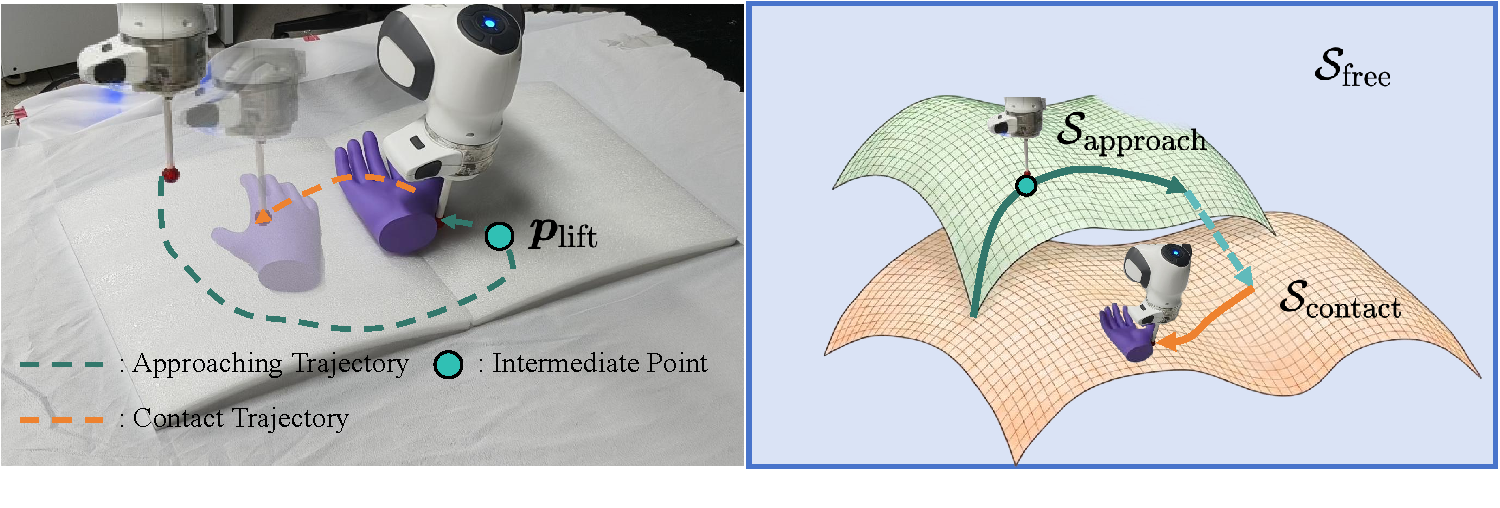
\includegraphics[width=\columnwidth]{figures/cpo_problem_def.pdf}}
\caption{(a) Illustrative example of a feasible approach and contact trajectory. (b) Explanation of CPO in a geometric perspective. CPO can be characterized as operating over two manifolds: contact states in $\mathcal{S}_{\text{contact}}$ and  approaching trajectories on the manifold $\mathcal{S}_{\text{approach}}$ embedded in the contact-free state space $\mathcal{S}_{\text{free}}$. CPO must not only generate contact trajectories on $\mathcal{S}_{\text{contact}}$ but also address the gradient-sparse issue and generate trajectories on $\mathcal{S}_{\text{approach}}$.}
\label{fig:approaching_contact}
\end{figure}

\begin{figure}[!t]
 \centerline{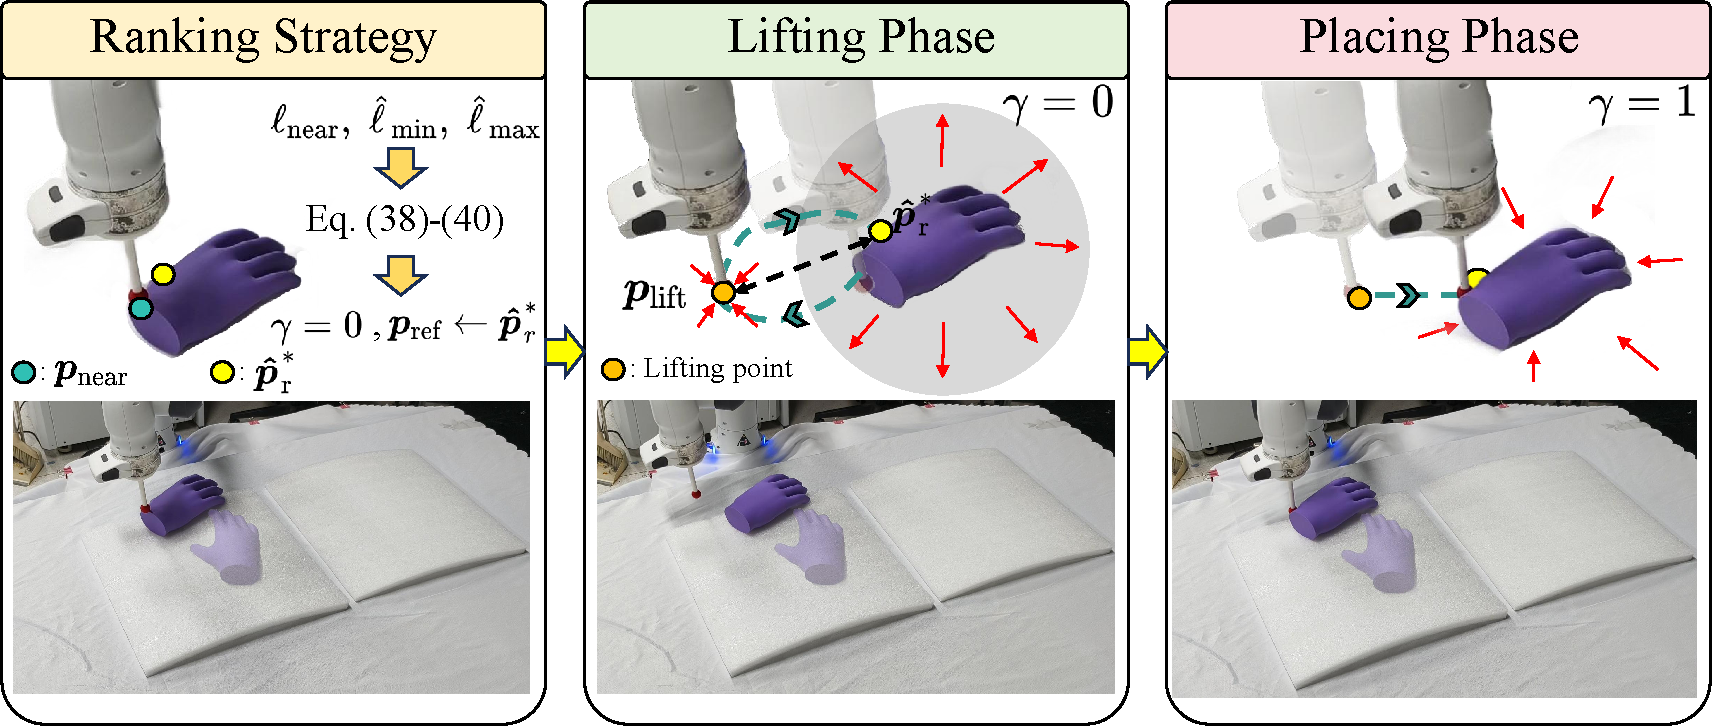
\includegraphics[width=\columnwidth]{figures/contact_planning_process.pdf}}
\caption{Illustration of the CPO-based contact planning module. (a) Ranking strategy. When $\boldsymbol{p}_{\text{near}}$ is evaluated infeasible, $\gamma$ turns to zero and $ \boldsymbol{p}_{\text{ref}} \gets \boldsymbol{\hat{p}}_r^*$. The evaluation runs continuously in real-time. (b) When $\gamma=0$,  the robot is guided by the potential field to $\boldsymbol{p}_{\text{lift}}$. (c) Once above $\hat{\boldsymbol{p}}_r^*$ or the nearest point $\boldsymbol{p}_{\text{ref}}$ to the robot is detected feasible via \eqref{equ:csqp}, $\gamma$ becomes 1 and an attractive potential is applied, guiding the robot to contact with the object.}
\label{fig:task_requirements}
\end{figure}

The formulation in \eqref{equ:cpo_formulation} preserves the favorable properties of the original CIMPC objective while enabling hybrid contact planning. Therefore, CPO can be interpreted as a prior-guided contact planning framework. We state the following lemma.


\subsection{Solvers of CPO} 

Since CPO specifies the optimization formulation rather than a specific solver, various reactive motion planners can be adopted to generate contact trajectories. Below, we present two solvers employed in our experiments.


\subsubsection{Operational-Space Control}
\label{sec:osc_control}
We simplify the full-order contact planning problem to an end-effector point contact planning problem, avoiding high-DoF robot trajectory optimization. The resulting joint torques are generated by operational space control (OSC) \cite{nakanishi2008operational} to track the CPO output. Specifically, the state in \eqref{equ:cpo_formulation} is reduced to $\boldsymbol{s} \in \mathbb{R}^{10}$, consisting of the object position, object orientation represented by a quaternion, and the end-effector position $\boldsymbol{p}_{\text{ee}} \in \mathbb{R}^3$. Solving \eqref{equ:cpo_formulation} yields the control input $\boldsymbol{u} = \Delta \boldsymbol{p}_{\text{ee}}$.

Given the desired pose $(\boldsymbol{p}_d, \boldsymbol{R}_d)$ with $\boldsymbol{p}_d=\boldsymbol{p}_{\text{ee}}+\boldsymbol{u}$ and a preset $\boldsymbol{R}_d$, the position and orientation errors are computed as $\boldsymbol{e}_{\text{pos}} = \boldsymbol{u},
$ and $\boldsymbol{e}_{\text{R}} = \boldsymbol{R}_{\text{ee}}^\top \boldsymbol{R}_d$.
Converting $\boldsymbol{e}_{\text{R}}$ to quaternion form gives $\boldsymbol{e}_{\text{quat}} =
\begin{bmatrix}
\boldsymbol{\epsilon}_e, 
\eta_e
\end{bmatrix}^\top
\in \mathbb{R}^4$,
and after sign correction,
\begin{equation}
\boldsymbol{e}_{\text{quat}} \leftarrow
\begin{cases}
\boldsymbol{e}_{\text{quat}}, & \eta_e \ge 0,\\
-\boldsymbol{e}_{\text{quat}}, & \eta_e < 0,
\end{cases}
\qquad
\boldsymbol{e}_{\text{rot}} = -\boldsymbol{R}\boldsymbol{\epsilon}_e.
\end{equation}
By defining
$\boldsymbol{e}_{\text{pose}} =
\begin{bmatrix}
\boldsymbol{e}_{\text{pos}},
\boldsymbol{e}_{\text{rot}}
\end{bmatrix}^\top$,
the task-space and null-space torques are given by:
\begin{align}
\boldsymbol{\tau}_{\text{task}} &=
\boldsymbol{J}^{\top}(\boldsymbol{q})
\left(
-\boldsymbol{K}_x \boldsymbol{e}_{\text{pose}}
-\boldsymbol{D}_x \dot{\boldsymbol{x}}
\right), \\
\boldsymbol{\tau}_{\text{null}} &=
\left(
\boldsymbol{I} - \boldsymbol{J}^{\top}(\boldsymbol{J}^{\top})^{\dagger}
\right)
\left(
\boldsymbol{K}_{q}(\boldsymbol{q}_{\text{init}} - \boldsymbol{q})
- 2\sqrt{\boldsymbol{K}_{q}}\,\dot{\boldsymbol{q}}
\right),
\end{align}
and the final control torque is
$\boldsymbol{\tau} =
\boldsymbol{\tau}_{\text{task}}
+ \boldsymbol{\tau}_{\text{null}}
+ g(\boldsymbol{q})$. This controller is used in all simulations and real-world experiments in Section \ref{sec:experiment}, and is suitable for tasks such as tabletop manipulation, where high orientation diversity is not critical.

\subsubsection{Sampling-based Motion Planner}

Another formulation is to directly solve the full-order planning problem of the robot. In this case, the state in \eqref{equ:cpo_formulation} is given by $\boldsymbol{x} \in \mathbb{R}^{7 + n_{\text{DoF}}}$, where $n_{\text{DoF}}$ denotes the number of robot DoFs. For this class of problems, we employ sampling-based MPC methods as the solver, such as MPPI \cite{williams2015model}. Recent studies  have demonstrated the impressive performance of MPPI in solving high-dimensional optimization problems for redundant robots, enabling real-time computation while avoiding issues related to gradient-based methods. The cost function is defined in the same manner as in the previous formulation, except that $\boldsymbol{p}_{\text{ee}}$ is computed via forward kinematics for the full-order problem. 

\section{Experiment: Nonprehensile Manipulation}
\label{sec:experiment}
\label{sec:experiment_ii}

This section evaluates the SCSP framework through nonprehensile manipulation experiments, which represent a class of contact-rich manipulation tasks characterized by frequent contact-state transitions and unstable control. The tasks consist of on-ground rotation and on-ground flipping. On-ground rotation requires the robot to move an object to a target pose on the ground through 2D pushing and rotating, whereas on-ground flipping involves 6D manipulation. We select a set of irregularly shaped objects from the ContactDB dataset \cite{brahmbhatt2019contactdb} for validation. The objects are initialized at random poses with
$x_{\text{init}}, y_{\text{init}} \in [-0.3, 0.3]$ m,
and Euler angles \rev{$(\phi_{\text{init}}, \theta_{\text{init}}, \varphi_{\text{init}})$}
uniformly sampled from $[-\pi, \pi]$ rad. We define the conditions of task success as:
\begin{equation}
 \left\| \boldsymbol{p}_o - \boldsymbol{p}_{\text{goal}} \right\|
\le 0.02 \,\text{[m]}, \
1 - (\boldsymbol{\psi}_{\text{goal}}^\top \boldsymbol{\psi}_o)^2
\le \textcolor{red}{0.015}, \label{eq:pose_success}
\end{equation}
\textcolor{red}{where the orientation tolerance corresponding to the quaternion error threshold is $14.1^\circ$.} A trial is considered successful if the conditions are satisfied within 2500 rollout steps.

Simulations are conducted in \texttt{MuJoCo} \cite{todorov2012mujoco} and \texttt{IsaacGym} \cite{makoviychuk2021isaac} with a fixed integration time step \textreplace{$h=0.02 \text{s}$}{$h=0.002\,\mathrm{s}$}. For the sampling method in our CSO module, we use \texttt{CoACD} \cite{wei2022approximate} for convex decomposition of the objects and \texttt{trimesh} for mesh processing and local frame construction. \rev{CSO is solved using GPU-parallel CEM,} while CPO is solved using \texttt{acados} SQP-RTI with HPIPM and a solver tolerance of $10^{-4}$. Unless otherwise stated, experiments are conducted on a desktop computer with an Intel i7-13620H processor, 32 GB RAM, and an NVIDIA GeForce RTX 5090 GPU.

We applied randomization to the environment and object parameters. The friction coefficients of the object $\mu_{\text{o}}$, fingertip $\mu_{\text{r}}$, and ground $\mu_{\text{env}}$ are all set to 0.5 with random perturbations of $\pm 0.2$. The object mass is randomly sampled from the discrete set
$\{0.01,0.1,1.0,10.0\}$ kg \textcolor{red}{with equal probability for each trial}. We set $\boldsymbol{M}_o=\text{diag}(50,50,50,0.05,0.05,0.05)$ and $\boldsymbol{K}_r=300 \boldsymbol{I}_7$, and the dynamic parameters used in SCM are not measured precisely, but are roughly set to their mean values.

For CSO, the default configuration samples $n_s=70$ candidate contacts, retains the two lowest-cost candidates, and \rev{uses a one-step prediction ($T=1$) with 20 GPU-parallel CEM iterations}. CSO and CPO share a prediction step of \textreplace{$0.02\,\mathrm{s}$}{$h=0.002\,\mathrm{s}$} and pose weights $w_{\mathrm{pos}}=500$ and $w_{\mathrm{quat}}=20$. CSO uses a $3\,\mathrm{N}$ force-command limit corresponding to $\hat{\lambda}^{n}_{\max}\approx1.59\,\mathrm{N}$ under the configured friction pyramid. CPO uses $N=5$, componentwise control bounds $|u_j|\leq0.005\,\mathrm{m}$, and weights $w_{\mathrm{lp}}=1$, $w_u=50$, and $w_{\mathrm{cso}}=10$. Its lifting and reference-contact attraction weights are both 20, while the repulsive-field term is disabled. \addrev{The lift--cross--drop path uses clearance margins $d_{\text{top}}=0.025\,\mathrm{m}$ and $d_{\text{ref}}=0.015\,\mathrm{m}$ and a per-cycle step bound of $0.005\,\mathrm{m}$ on $\boldsymbol{p}_{\text{lift}}$. The bounding box defining $z_{\text{top}}$ is the axis-aligned bounding box of the object mesh in its body frame, with center $\boldsymbol{c}$ and half-extents $\boldsymbol{e}$; it is rotated with the estimated object pose and $z_{\text{top}}=(\boldsymbol{p}_o+\boldsymbol{R}_o\boldsymbol{c})_z+\sum_i|R_{o,zi}|\,e_i$ is the top of the resulting oriented box, so \rev{$z_{\text{c}}$} follows the object's current orientation. Segment switching uses tolerances of $0.004\,\mathrm{m}$ on the height \rev{$z_{\text{c}}$} and $0.008\,\mathrm{m}$ on the horizontal distance to the waypoint; the latched waypoint is released when the end-effector is within $0.012\,\mathrm{m}$ of the target or the object moves by more than $0.015\,\mathrm{m}$.} \textreplace{During the flipping stage, the orientation error measures alignment of the object's target upright axis with the world vertical, leaving yaw unconstrained. Let $\boldsymbol{a}_g=\boldsymbol{R}(\boldsymbol{x}_{\mathrm{goal}})^\top e_z$, where $e_z=[0,0,1]^\top$. The normalized upright error is $\ell_{\mathrm{up}}(\boldsymbol{x}_o)$$ = \frac{1}{2}\left[1-e_z^\top\boldsymbol{R}(\boldsymbol{x}_o)\boldsymbol{a}_g\right]$. The flipping-stage object cost is $\ell_{\mathrm{cso}}=500\ell_{\mathrm{pos}}+20\ell_{\mathrm{up}}$, i.e., $\ell_{\mathrm{pose}}$ in \eqref{equ:obj_pose_cost} with the quaternion-error term replaced by this yaw-free upright error. Here $\ell_{\mathrm{pos}}=\|\boldsymbol{p}_o-\boldsymbol{p}_{\mathrm{goal}}\|^2$, except for the Stanford bunny, which uses \resizebox{0.96\columnwidth}{!}{$\ell_{\mathrm{pos}}=\max(\|\boldsymbol{p}_{o,xy}-\boldsymbol{p}_{\mathrm{goal},xy}\|-0.08\,\mathrm{m},0)^2$} to allow vertical motion and planar displacement within an $8\,\mathrm{cm}$ radius during flipping.}{All objects use the same full-position and quaternion objective $\ell_{\mathrm{pose}}$ in \eqref{equ:obj_pose_cost}, with $w_{\mathrm{pos}}=500$ and $w_{\mathrm{quat}}=20$, for both rotation and flipping.}

From Table \ref{tab:comparison}, \rev{we select methods that are applicable to 6D manipulation and can manipulate objects with arbitrary geometries, rather than being restricted to regular shapes,} as baselines, including:
\begin{itemize}
 \item \rev{\textbf{DyWA}~\cite{lyu2025dywa}: An end-to-end 6D nonprehensile policy evaluated on unseen object geometries using the released single-view student policy in \texttt{IsaacGym}.}
 \item \rev{\textbf{ContactSDF}~\cite{yang2024contactsdf}: A differentiable multi-contact model based on signed distance functions (SDFs), which provides closed-form collision detection and time-stepping prediction for contact-rich manipulation.}
 \item \rev{\textbf{STOCS-3D}~\cite{zhang2025simultaneous}: An offline method that jointly optimizes contact selection and a contact-implicit trajectory optimization (CITO) problem for 3D manipulation. We use STOCS-3D to generate the CITO trajectory offline and execute the resulting trajectory with operational-space control (OSC).}
 \item \rev{\textbf{Sampling}~\cite{venkatesh2025approximating}: A hierarchical method that samples candidate contacts and evaluates them with a lower-level CIMPC controller.} \rev{We use the released implementation with its original C3 contact model, Gurobi MIQP solver, and contact-selection method.}
 \item \rev{\textbf{CF-MPC}~\cite{jin2024complementarity}: A complementarity-free MPC method with a closed-form contact model and limited explicit contact-selection capability.}
\end{itemize}

\subsection{Robot Manipulation in Simulation}\label{sec:robot_manipulation}

We evaluate SCSP in redundant robot manipulation tasks. Compared with a floating end-effector, contact problems for redundant robots introduce complex kinematic constraints. In the experiments, we demonstrate the superiority of SCSP and validate the soundness of our framework.

\begin{figure}[!t]
 \centerline{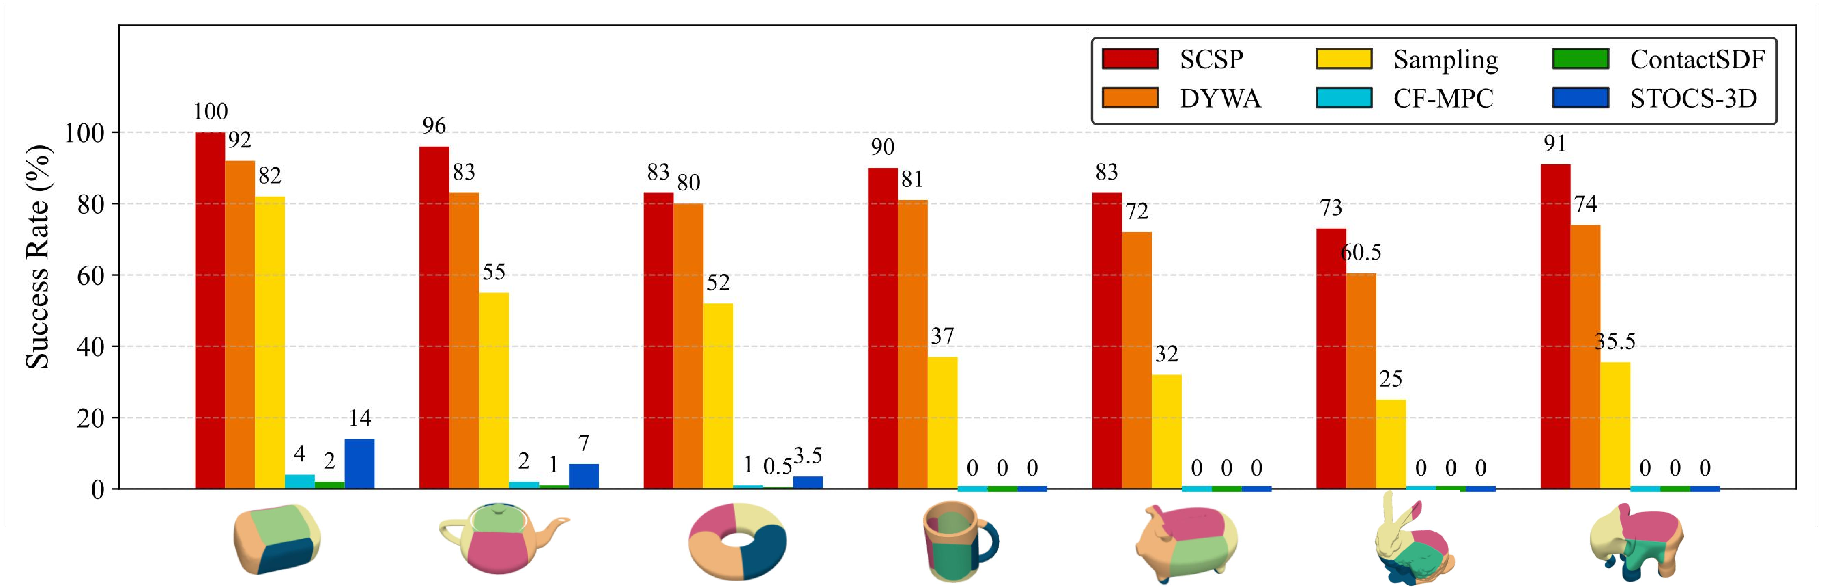
\includegraphics[width=\columnwidth]{figures/franka_exp.pdf}}
\caption{Experimental results of robot manipulation in simulation. SCSP significantly outperforms other model-based methods and exceeds the performance of well-trained learning-based methods.}
\label{fig:results_panda}
\end{figure}

Due to the strong dependencies of the source code released for DyWA, which are difficult to transfer, we follow its setup and conduct all experiments in \texttt{IsaacGym} for consistency, with the same simulation settings described above. All methods use our link-mounted sphere as the end-effector to replicate point contacts. Since DyWA uses the Franka gripper, we adjust the link length so that the sphere’s center coincides with the gripper’s center. The Cartesian stiffness $\boldsymbol{K}_x=\text{diag}(1000,1000,1000,50,50,50)$ and $\boldsymbol{D}_x=\sqrt{2\boldsymbol{K}_x}$. \rev{All methods use the same settings as above, with the control dimension set by each method\textquotesingle s formulation.} $\boldsymbol{p}_{\text{ee}}$ is obtained via differentiable forward kinematics.

\begin{table*}[t]
\centering
\caption{Comparison and ablation results for nonprehensile manipulation tasks in the robot experiments}
\label{tab:all_data}
\setlength{\tabcolsep}{2pt}
\renewcommand{\arraystretch}{0.95}
\resizebox{\linewidth}{!}{
\begin{tabular}{ll*{6}{c}|*{7}{c}}
\toprule[1pt]
\multirow{2}{*}{\textbf{Task}} & \multirow{2}{*}{\textbf{Metric}} & \multicolumn{6}{c|}{\textbf{Comparison}} & \multicolumn{7}{c}{\textbf{Ablation}} \\
\cmidrule(lr){3-8} \cmidrule(lr){9-15}
 & & \textbf{SCSP*} & \textbf{DyWA} & \textbf{ContactSDF} & \textbf{STOCS-3D} & \textbf{Sampling} & \textbf{CF-MPC} & \textbf{A1} & \textbf{A2} & \textbf{A3} & \textbf{A4} & \textbf{A5} & \textbf{A6} & \textbf{A7} \\
\midrule
\multirow{5}{*}{Rotation} & Success Rate & \textbf{0.95} & 0.86 & 0.01 & 0.07 & 0.52 & 0.01 & 0.37 & 0.06 & 0.57 & 0.66 & 0.89 & 0.00 & 0.17 \\
 & Execution Time (s) & 15.16$\pm$11.82 & 18.12$\pm$18.46 & 20.12 $\pm$ 1.12 & 19.36 $\pm$ 8.75 & 18.97$\pm$12.91 & 13.18$\pm$8.67 & 25.31$\pm$11.03 & \textbf{12.74$\pm$0.14} & 10.91$\pm$9.15 & 20.77$\pm$9.82 & 19.06$\pm$8.53 & -- & 16.21$\pm$1.90 \\
 & Planning Time (ms) & 21.12$\pm$10.27 & 31.00$\pm$7.67 & 22.30$\pm$11.17 & (5.93$\pm$5.30)$\times$10\textsuperscript{5} & 108.12 & 11.32 $\pm$6.27  & 13.55$\pm$10.42 & 13.91$\pm$9.52 & 15.21$\pm$7.43 & 99.94$\pm$61.10 & 612.53$\pm$168.13 & 81.38$\pm$11.62 & \textbf{12.09$\pm$2.23} \\
 & Obj. Pos. Error (m) & 0.05$\pm$0.11 & 0.07$\pm$0.13 & 0.06$\pm$0.03 & 0.17$\pm$0.07 & 0.08$\pm$0.07 & 0.20$\pm$0.05 & 0.11$\pm$0.13 & 0.17$\pm$0.08 & 0.09$\pm$0.09 & \textbf{0.04$\pm$0.06} & 0.06$\pm$0.14 & 0.29$\pm$0.13 & 0.29$\pm$0.16 \\
 & Obj. Quat. Error & \textbf{0.01$\pm$0.02} & 0.02$\pm$0.02 & 0.24$\pm$0.34 & 0.28$\pm$0.37 & 0.30$\pm$0.37 & 0.21$\pm$0.16 & 0.19$\pm$0.30 & 0.31$\pm$0.37 & 0.18$\pm$0.32 & 0.07$\pm$0.19 & 0.07$\pm$0.20 & 0.58$\pm$0.33 & 0.30$\pm$0.37 \\
\midrule
\multirow{5}{*}{Flipping} & Success Rate & \textbf{0.81} & 0.69 & 0.00 & 0.00 & 0.39 & 0.01 & 0.19 & 0.00 & 0.37 & 0.26 & 0.60 & 0.00 & 0.00 \\
 & Execution Time (s) & 18.75$\pm$9.79 & 20.56$\pm$12.96 & -- & -- & 22.68$\pm$12.95 & \textbf{14.56$\pm$6.37} & 22.05$\pm$9.36 & -- & 23.60$\pm$11.86 & 22.71$\pm$12.59 & 24.23$\pm$11.50 & -- & -- \\
 & Planning Time (ms) & 20.91$\pm$8.03 & 31.00$\pm$7.67 & 23.22$\pm$12.22 & (2.39$\pm$1.25)$\times$10\textsuperscript{5} & 102.23$\pm$29.72 & 10.16 $\pm$ 9.42 & 13.94$\pm$9.23 & 14.59$\pm$9.34 & 15.80$\pm$11.85 & 132.95$\pm$49.02 & 577.81$\pm$113.82 & 81.75$\pm$10.63 & \textbf{12.86$\pm$2.90} \\
 & Obj. Pos. Error (m) & \textbf{0.04$\pm$0.05} & 0.13$\pm$0.17 & 0.20$\pm$0.09 & 0.17$\pm$0.04 & 0.10$\pm$0.05 & 0.19$\pm$0.05 & 0.16$\pm$0.14 & 0.15$\pm$0.05 & 0.12$\pm$0.12 & 0.09$\pm$0.09 & 0.11$\pm$0.15 & 0.24$\pm$0.08 & 0.35$\pm$0.16 \\
 & Obj. Quat. Error & \textbf{0.02$\pm$0.01} & 0.05$\pm$0.06 & 0.87$\pm$0.19 & 0.79$\pm$0.25 & 0.40$\pm$0.38 & 0.37$\pm$0.19 & 0.38$\pm$0.41 & 0.73$\pm$0.32 & 0.47$\pm$0.41 & 0.46$\pm$0.22 & 0.29$\pm$0.40 & 0.76$\pm$0.30 & 0.80$\pm$0.25 \\
\bottomrule[1pt]
\end{tabular}
}
\end{table*}

\begin{figure*}
 \centerline{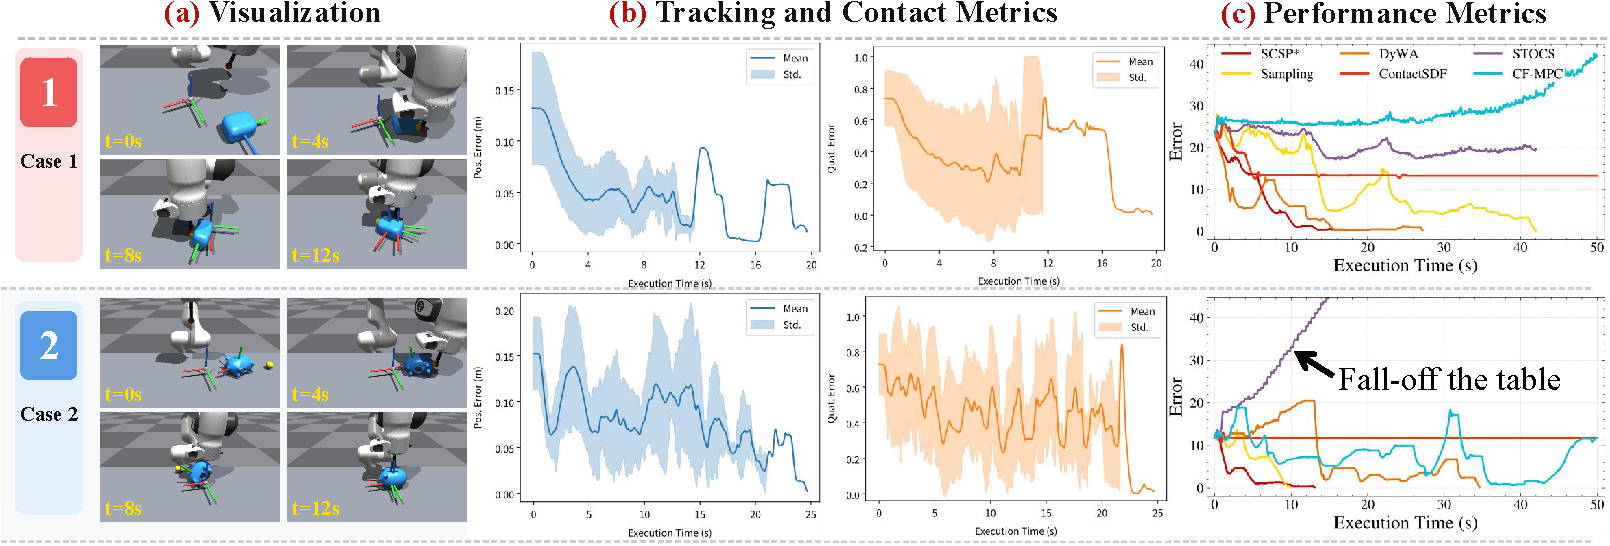
\includegraphics[width=\textwidth]{figures/franka_exp_result.pdf}}
\caption{Nonprehensile manipulation experiments in simulation. (a): Snapshots of SCSP in the robot experiments, where the goal pose is visualized either transparently or as a floating coordinate frame. (b): The mean and standard deviation curves of the position and orientation errors over steps across 10 SCSP trials. (c) The pose error $\ell_{\text{pose}}$ of different methods during manipulation. The comparison methods either require longer execution time or fail due to local minima or solver failures.}
\label{fig:simulation_data}
\end{figure*}

\begin{figure}
 \centerline{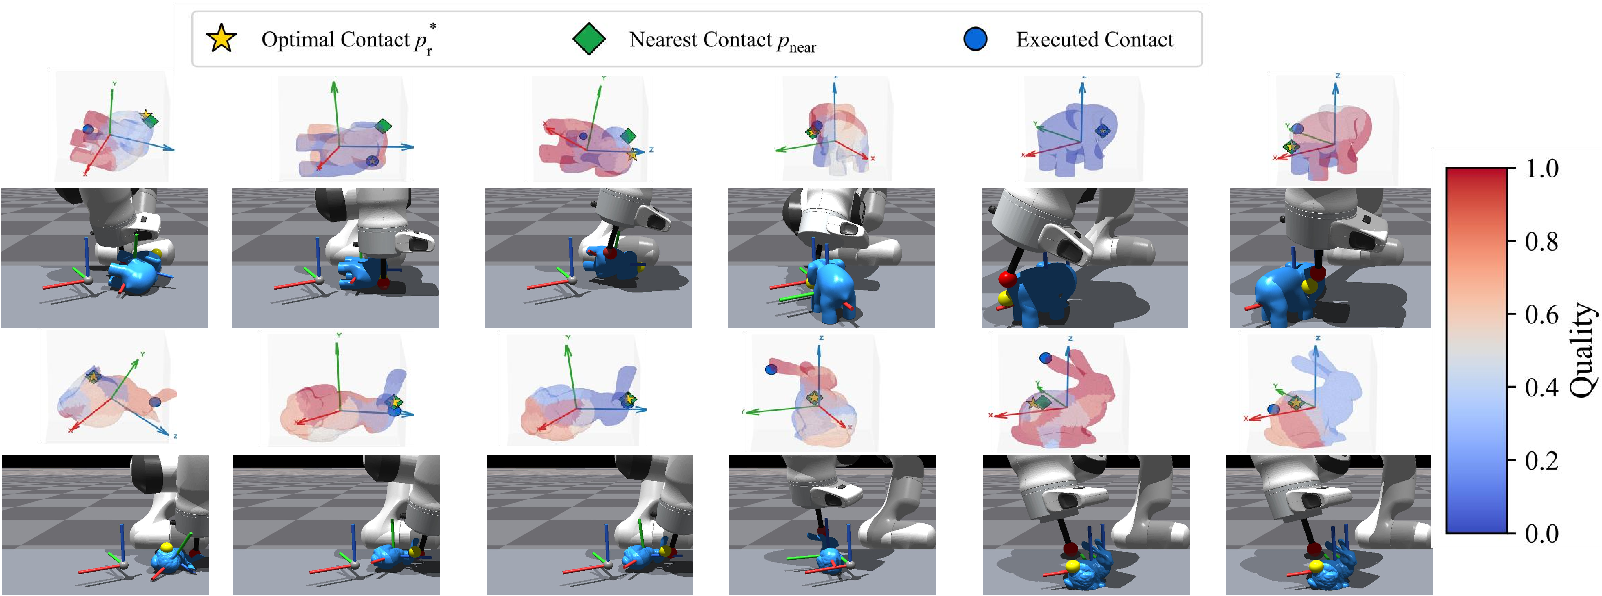
\includegraphics[width=\columnwidth]{figures/contact_map.pdf}}
\caption{Visualization of the contact map during the elephant and bunny flipping tasks. Red indicates a larger cost reduction predicted by CSO and thus higher contact quality.}
\label{fig:contact_map}
\end{figure}

The experimental results are shown in Fig. \ref{fig:results_panda}, Fig. \ref{fig:simulation_data}, and Table \ref{tab:all_data}. SCSP achieves a higher success rate than other model-based algorithms and outperforms DyWA on all objects except the torus. Additionally, SCSP achieved the shortest execution time \rev{among the comparison methods (the shorter times of A2 and CF-MPC are averaged over very few successful trials)}, demonstrating that SCSP can generate correct contact locations through CSO, thereby efficiently minimizing the pose cost of the object. SCSP also achieved the smallest convergence position error and quaternion error \rev{among the comparison methods, while A4 and A5 attain comparable errors at a much higher planning cost}. Furthermore, we observed that during experiments, DyWA tends to flip objects by pressing the edges of the top surface, whereas our method makes more comprehensive decisions regarding whether to lift the object by pushing the bottom or by pressing the top. Although many flipping tasks can be accomplished through pressing, for certain objects (such as elongated objects), the pressing approach requires applying substantial torque to the object and demands sufficiently high coefficients of friction. Based on our observations, the global contact selection mechanism in CSO enables SCSP to exhibit greater diversity in its manipulation behaviors compared with other methods, rather than converging to a single strategy. \rev{Fig.~\ref{fig:contact_map} shows the actual CSO cost evaluation and contact selection during flipping: the executed contact switches between $\boldsymbol{p}_{\text{near}}$ and $\hat{\boldsymbol{p}}_r^*$, i.e., the ranking strategy does not always select either one.}

We further validated the impact of different numbers of sampled candidate points on performance. As shown in Table \ref{tab:cso_sampling}, when the number of sampled points reaches 70, nearly the highest success rate is achieved with relatively low SCSP computation time. As the number of sampled points continues to increase, the success rate plateaus and computational efficiency deteriorates. This indicates that increasing the number of sampled points does not necessarily improve performance. There exists an optimal convergence value. For nonprehensile manipulation tasks, 70 to 100 sampled points are sufficient to characterize the geometric features of object geometries.

\begin{table}[t]
\centering
\caption{Evaluation of the effect of the number of candidate points}
\label{tab:cso_sampling}
\begin{tabular}{lccccc}
\toprule
\textbf{Sampling numbers in CSO} & \textbf{5} & \textbf{10} & \textbf{70} & \textbf{120} & \textbf{500} \\
\midrule
\textbf{Avg. Success Rate} & 0.25 & 0.59 & \textbf{0.88} & \textbf{0.88} & 0.85 \\
\textbf{SCSP Computation Time} (ms) & \textbf{10.92} & 10.97 & 12.52 & 12.91 & 13.85 \\
\bottomrule
\end{tabular}
\end{table}

\begingroup
\color{red}
\subsection{Ablation Studies}

We ablate the ranking strategy, CSO, and CPO under the same experimental setup as in Section~\ref{sec:robot_manipulation} to demonstrate their contributions. We also examine contact-model fidelity and the feasibility of CSO-generated contact trajectories.

\subsubsection{Functional Analysis of SCSP Components}
\label{sec:component_ablation}
\textbf{Ranking strategy (A1--A2):} CPO strictly follows CSO-optimal guidance $p_r^*$ (A1) or always executes the nearest contact $p_{\text{near}}$ (A2).

\textbf{CSO (A3--A5):} \rev{A3 replaces SCM with a coarse contact model that encloses the object in an oriented bounding box (OBB), ignores object--environment contact, and evaluates candidate contact locations solely based on the object pose error. This variant assesses the model fidelity needed to provide useful contact priors.} A4 replaces SCM with MuJoCo's QP-based contact model; \rev{A5 directly applies CMA-ES to solve \eqref{equ:outer_loop} and obtain $(\boldsymbol{p}_{\mathrm r}^*,\boldsymbol{\lambda}_{\mathrm r}^*)$, without sampling, constructing, or evaluating a candidate contact set. The SDF-distance constraint $d_{\mathrm{SDF}}(\boldsymbol{p}_{\mathrm r})=0$ enforces that every optimized contact point lies on the object surface.}

\textbf{CPO (A6--A7):} A6 removes the phase-dependent attraction and repulsion potentials and directly optimizes motion trajectories; \textcolor{red}{A7 removes contact guidance from CPO and solves the resulting problem with MPPI~\cite{williams2015model}: the ranking strategy and the lifting phase are removed, and the objective in \eqref{equ:cpo_formulation} retains only the attraction toward $\boldsymbol{p}_{\text{near}}$ in \eqref{eq:placing_cost} and the object cost $\ell_{\text{pose}}$, with the same cost weights and horizon as CPO. MPPI samples end-effector displacements under the same $f_{\text{cf}}$ and control bounds as CPO, with $N=5$, 128 samples, one iteration, noise $\sigma=0.003\,\mathrm{m}$, and temperature $0.005$.} Table~\ref{tab:all_data} summarizes the results.

A1 and A3 substantially outperform A2, demonstrating the importance of contact guidance over purely local contact selection. However, frequent contact switching in A1 makes effective contact maneuvers difficult to complete, leading to timeouts. \rev{Even the coarse contact model in A3 yields substantial performance gains, suggesting that useful contact priors do not require detailed contact modeling.} A4 and A5 show that higher model fidelity or more refined optimization does not necessarily improve task success. Compared with CPO's cost formulation, directly solving the full trajectory planning problem in A6 imposes a greater computational burden, reducing success rates and substantially increasing planning time. Despite using MPPI for stronger exploration \textcolor{red}{of the same CPO problem without contact guidance}, A7 still achieves low success rates, indicating that increased exploration alone cannot effectively replace contact guidance.

We also test sensitivity to the acceptance threshold $\bar{\rho}$ and the EMA coefficient $\beta$ (Fig.~\ref{fig:sensitivity}). Setting $\bar{\rho}=0$ accepts nearby contacts without filtering their quality, recovering A2, whereas $\bar{\rho}=1$ restricts acceptance to optimal contacts, corresponding to A1. Smaller $\bar{\rho}$ values make nearby contacts easier to accept. Setting $\beta=1$ disables smoothing and permits abrupt changes between consecutive decisions, whereas smaller positive values provide stronger smoothing but slow the response; $\beta=0$ prevents the filtered \textcolor{red}{trigger $\bar{\kappa}_t$} from updating. \rev{The sweep results support the default settings $\bar{\rho}=0.7$ and $\beta=0.2$, which are used in the experiments below.}

\begin{figure}[!t]
\color{red}
\def\normalcolor{\color{red}}
 \centerline{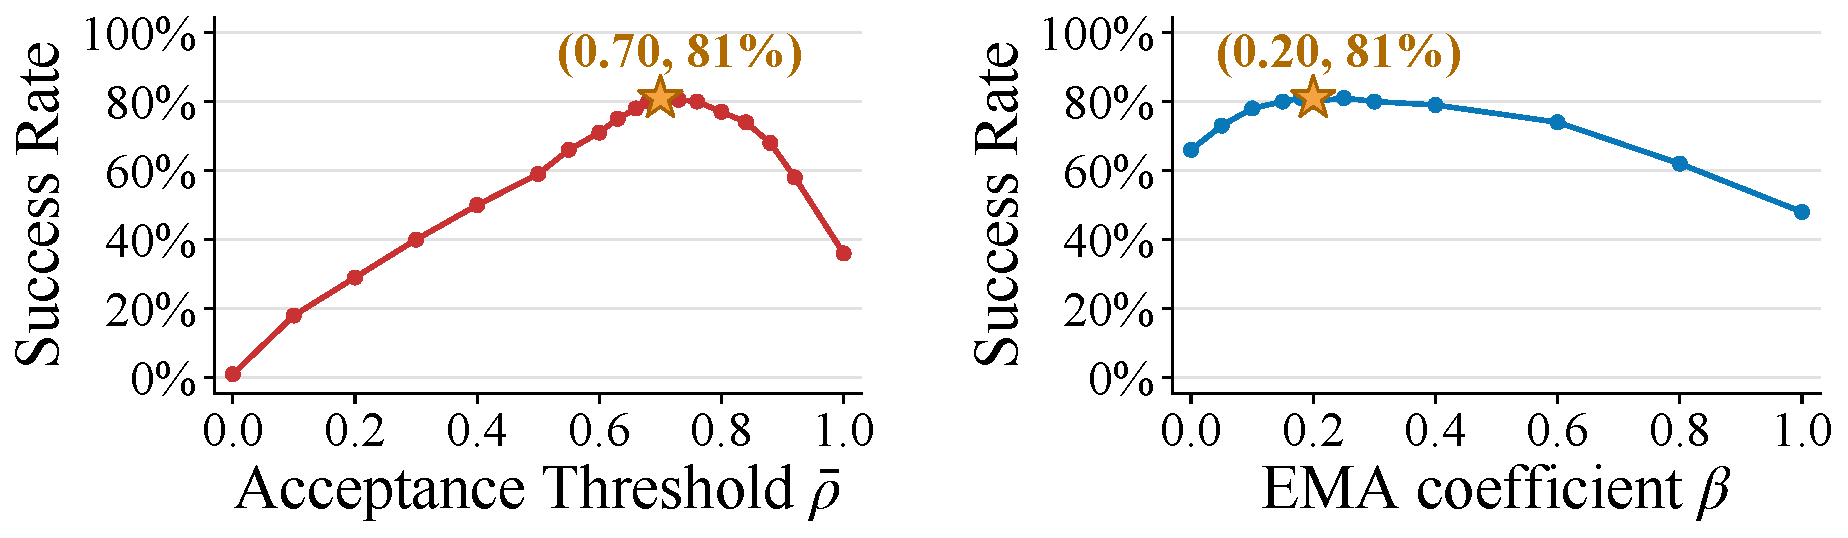
\includegraphics[width=\columnwidth,trim=0 6bp 0 0,clip]{figures/fig_sensitivity.pdf}}
\caption{\rev{Sensitivity of the measured success rate} to the acceptance threshold $\bar{\rho}$ and EMA coefficient $\beta$. Each parameter is varied independently while the others are fixed at their default values.}
\label{fig:sensitivity}
\vspace{-10pt}
\end{figure}

\subsubsection{Contact Model Evaluation}
\label{sec:scm_evaluation}

We evaluate contact-model fidelity and the feasibility of the resulting ideal contact trajectories. We report the linear- and angular-velocity errors between SCM and the corresponding MuJoCo and IsaacGym references under contact transition, sliding, sticking, and rotation/flipping rollouts. \rev{The contact state of a sample is determined from the loaded contacts of the reference input state: \emph{contact transition} if any loaded contact has a normal relative speed above $0.01\,\mathrm{m/s}$ (impact or lift-off); otherwise \emph{sliding} if any loaded contact slips faster than $1\,\mathrm{mm/s}$; otherwise \emph{sticking}. The three states partition all contact situations; the transition samples comprise impact and lift-off initial states (32 and 16 per object), and airborne states are excluded.} For the contact-mode measurements, samples are further grouped by the reference active-contact count $n_c\in\{1,2,\geq3\}$. The benchmark uses seven objects, 32 initial states per object and contact state, and 10 rollout windows per rollout state. \rev{In the rollout columns, every engine is reset to the MuJoCo reference state at each of the 250 steps of a window and advanced once, so all columns report one-step errors from a common reference state and differ only in the state distribution of the rotation and flipping manoeuvres. The larger IsaacGym transition errors and the spread of its rollout columns come from the depenetration response of PhysX when it is initialized at the slightly penetrating states produced by MuJoCo's soft contacts.} \rev{Table~\ref{tab:scm_velocity_error} shows that, apart from this state, the linear errors stay at the centimetre-per-second level and the angular errors below $0.3\,\mathrm{rad/s}$ in sticking and about $1\,\mathrm{rad/s}$ otherwise; outside transition they vary little with $n_c$. Per object (Fig.~\ref{fig:scm_error_heatmap}), the SCM--MuJoCo linear errors stay below $0.07\,\mathrm{m/s}$ for all objects and only the IsaacGym transition row is elevated.}
For SCM, we set $\epsilon=10^{-8}$ and \rev{$T=10^{-4}\,\mathrm{N\,s}$ and report the one-step prediction of \eqref{eq:scm_single_step_projection} with $K=3$ sweeps at $h=0.002\,\mathrm{s}$.} Initial poses are obtained by native MuJoCo settling.

We then evaluate whether the ideal contact trajectories generated by each model can achieve the manipulation goals under the success criteria in \eqref{eq:pose_success}. The results are shown in Table~\ref{tab:cso_contact_guidance}. \rev{M1 and M2 denote the native contact models of MuJoCo (QP-based) and IsaacGym (PhysX), each used as the CSO model and rolled out in its own engine. Ideal control applies the CSO wrench $\boldsymbol{\lambda}^*$ directly at the optimal contact for one step $h$ before replanning, bypassing the robot;} we report manipulation success, planning time, and execution steps under synchronous inference without observation latency. \rev{Each model is evaluated on 100 rotation and 100 flipping trials with the setup and success criteria of Section~\ref{sec:robot_manipulation}.} Planning time and execution steps are mean $\pm$ std, with planning time pooled over planning rounds and execution steps taken over successful trials. \rev{All models reach an ideal success of 0.99--1.00, so each yields contact guidance that can succeed despite the errors in Table~\ref{tab:scm_velocity_error}; inside CSO, however, SCM plans an order of magnitude faster and attains the higher deployed success in both engines.}

\begin{table*}[t]
\centering
\caption{SCM velocity errors relative to MuJoCo and IsaacGym (mean $\pm$ std; linear in $\mathrm{m/s}$ and angular in $\mathrm{rad/s}$).}
\label{tab:scm_velocity_error}
\small
\setlength{\tabcolsep}{2pt}
\renewcommand{\arraystretch}{1.08}
\resizebox{\textwidth}{!}{
\begin{tabular}{@{}ll*{11}{c}@{}}
\toprule
\multirow{2}{*}{Comparison} & \multirow{2}{*}{Metric} & \multicolumn{3}{c}{Contact transition} & \multicolumn{3}{c}{Sliding} & \multicolumn{3}{c}{Sticking} & \multicolumn{2}{c}{Rollout} \\
\cmidrule(lr){3-5}\cmidrule(lr){6-8}\cmidrule(lr){9-11}\cmidrule(lr){12-13}
 & & $n_c=1$ & $n_c=2$ & $n_c\geq3$ & $n_c=1$ & $n_c=2$ & $n_c\geq3$ & $n_c=1$ & $n_c=2$ & $n_c\geq3$ & Rotation & Flipping \\
\midrule
\textcolor{red}{SCM--MuJoCo} & \textcolor{red}{Linear} & \textcolor{red}{0.01$\pm$0.01} & \textcolor{red}{0.03$\pm$0.02} & \textcolor{red}{0.02$\pm$0.02} & \textcolor{red}{0.04$\pm$0.02} & \textcolor{red}{0.06$\pm$0.03} & \textcolor{red}{0.06$\pm$0.03} & \textcolor{red}{0.00$\pm$0.00} & \textcolor{red}{0.00$\pm$0.00} & \textcolor{red}{0.00$\pm$0.00} & \textcolor{red}{0.01$\pm$0.03} & \textcolor{red}{0.02$\pm$0.14} \\
\textcolor{red}{SCM--MuJoCo} & \textcolor{red}{Angular} & \textcolor{red}{0.46$\pm$0.56} & \textcolor{red}{0.67$\pm$0.57} & \textcolor{red}{1.09$\pm$1.02} & \textcolor{red}{0.89$\pm$0.65} & \textcolor{red}{0.91$\pm$0.41} & \textcolor{red}{0.78$\pm$0.47} & \textcolor{red}{0.08$\pm$0.06} & \textcolor{red}{0.10$\pm$0.01} & \textcolor{red}{0.19$\pm$0.06} & \textcolor{red}{0.36$\pm$0.87} & \textcolor{red}{0.57$\pm$2.58} \\
\textcolor{red}{SCM--IsaacGym} & \textcolor{red}{Linear} & \textcolor{red}{0.42$\pm$0.35} & \textcolor{red}{0.37$\pm$0.32} & \textcolor{red}{0.37$\pm$0.33} & \textcolor{red}{0.01$\pm$0.00} & \textcolor{red}{0.01$\pm$0.01} & \textcolor{red}{0.02$\pm$0.01} & \textcolor{red}{0.00$\pm$0.00} & \textcolor{red}{0.01$\pm$0.00} & \textcolor{red}{0.01$\pm$0.01} & \textcolor{red}{0.04$\pm$0.12} & \textcolor{red}{0.14$\pm$0.75} \\
\textcolor{red}{SCM--IsaacGym} & \textcolor{red}{Angular} & \textcolor{red}{2.25$\pm$2.16} & \textcolor{red}{1.80$\pm$1.76} & \textcolor{red}{1.69$\pm$1.47} & \textcolor{red}{0.29$\pm$0.14} & \textcolor{red}{0.45$\pm$0.17} & \textcolor{red}{0.73$\pm$0.31} & \textcolor{red}{0.12$\pm$0.08} & \textcolor{red}{0.26$\pm$0.01} & \textcolor{red}{0.23$\pm$0.13} & \textcolor{red}{4.00$\pm$17.08} & \textcolor{red}{9.73$\pm$37.64} \\
\bottomrule
\end{tabular}
}
\end{table*}

\noindent

\begin{table}[t]
\centering
\caption{CSO contact-guidance performance.}
\label{tab:cso_contact_guidance}
\footnotesize
\resizebox{\columnwidth}{!}{
\setlength{\tabcolsep}{1.5pt}
\begin{tabular}{@{}l*{4}{c}@{}}
\toprule
\multirow{2}{*}{Metric} & \multicolumn{2}{c}{MuJoCo} & \multicolumn{2}{c}{IsaacGym} \\
\cmidrule(lr){2-3}\cmidrule(lr){4-5}
 & M1 & SCM & M2 & SCM \\
\midrule
Success (ideal) & 1.00 & 1.00 & 0.99 & 1.00 \\
Planning time (ms) & 27.76$\pm$5.68 & 2.18$\pm$0.75 & 22.82$\pm$3.00 & 2.30$\pm$0.79 \\
Execution steps & 160.74$\pm$98.06 & 216.96$\pm$126.33 & 305.09$\pm$287.05 & 379.00$\pm$465.02 \\
\midrule
Success (manip.) & 0.46 & 0.85 & 0.76 & 0.88 \\
\bottomrule
\end{tabular}
}
\end{table}

\begin{figure}[!t]
\centering
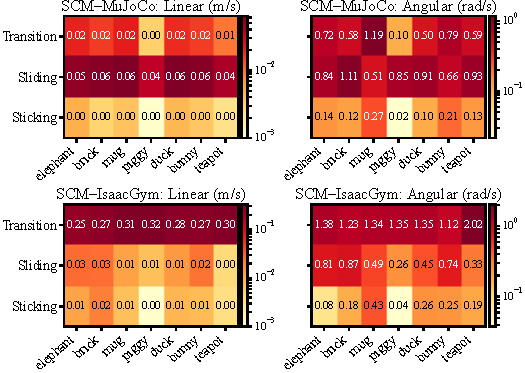
\includegraphics[width=\columnwidth]{figures/scm_prediction_heatmap.pdf}
\caption{\rev{Mean SCM prediction errors by object and contact state (log scale).}}
\label{fig:scm_error_heatmap}
\end{figure}

\subsubsection{Counterfactual Analysis of the Ranking Strategy}
\label{sec:ranking_ablation}
A1--A2 evaluate alternative contact-selection policies at the task level. We further assess the ranking strategy at individual decision points using matched counterfactual rollouts.

Inspired by reinforcement learning, we define a value for each contact-selection decision made by the ranking strategy. Let $r_T=\mathbb{I}(\mathrm{success})$ be the terminal reward. For a state $s_t$ and ranking decision $b$, the discounted rollout value is
\begin{equation}
J(s_t,b)=\mathbb{E}_{\tau\sim\pi(\cdot\mid s_t,b)}
\left[\textcolor{red}{\eta_{\mathrm{cf}}^{T}}\mathbb{I}(\mathrm{success})\right],
\end{equation}
where \textcolor{red}{$\eta_{\mathrm{cf}}=0.99$} and $T$ counts the actual execution steps from $s_t$ to trial termination, including all detour and contact-transition steps, rather than contact-selection events\textcolor{red}{, and the discount factor is denoted by $\eta_{\mathrm{cf}}$ to avoid confusion with the ranking phase variable $\gamma_t$ in \eqref{equ:ranking}}.

We sample 200 SCSP rollout trajectories and, in each, 10 decision points where the optimal contact location $p_r^*$ differs from $p_{\text{near}}$ (2000 decision points in total), and record the ranking strategy's decisions. At each selected state, we reverse the recorded decision, force the robot to execute the alternative contact strategy, and then resume SCSP until termination to obtain the reward and estimate the corresponding value. For example, during a contact-free phase, if SCSP selects the nearby contact, we instead force the robot to detour to $p_r^*$. During a contact phase, if SCSP decides to break the current contact and approach $p_r^*$, we instead force it to maintain the current contact. Let $J_{\mathrm{RS}}$ and $J_{\mathrm{cf}}$ denote the rollout values for the original and reversed decisions at $s_t$, respectively. Because SCSP replans at high frequency, a single-step decision deviation may have only a small effect on the overall trajectory. We therefore protect the perturbed decision from ranking overrides until the selected contact is established and evaluate its effect using the normalized advantage, defined as
\begin{equation}
\widetilde{A}(s_t)=
\begin{cases}
\displaystyle\frac{J_{\mathrm{RS}}-J_{\mathrm{cf}}}
{\max\{J_{\mathrm{RS}},J_{\mathrm{cf}}\}},
& \max\{J_{\mathrm{RS}},J_{\mathrm{cf}}\}>0,\\[4pt]
0, & \text{otherwise}.
\end{cases}
\end{equation}
Here $\widetilde{A}\in[-1,1]$, and $\widetilde{A}>0$ indicates that the ranking strategy is preferred. A value of $1$ ($-1$) means that only the RS (counterfactual) rollout succeeds. For two successful rollouts, this normalization depends only on the difference in their remaining completion steps, removing the common discount scale associated with long remaining trajectories.

We report the physical contact-switching frequency $f_{\mathrm{switch}}$, CSO-optimal contact-point switching frequency $f_r^*$, and selection probabilities $P(p_{\text{near}})$ and $P(p_r^*)$. These statistics are computed over the original sampled trajectories.
Table~\ref{tab:ranking_advantage} shows relatively balanced selection probabilities $P(p_{\text{near}})$ and $P(p_r^*)$ across the sampled trajectories, indicating that both contact strategies are extensively used. The CSO-optimal contact $p_r^*$ changes at approximately $5\,\mathrm{Hz}$, while physical contact switches occur at only about $0.2\,\mathrm{Hz}$. This suggests that the ranking strategy frequently mediates contact selection and filters changes in contact guidance. The fraction of positive advantages and the mean normalized advantage are particularly high for flipping ($90.68\%$ and $0.36$, respectively). These results are consistent with our observations: for rotation, the ranking strategy primarily improves efficiency by reducing detours; for flipping, it also helps maintain contact stability by avoiding frequent contact breaks.

\begin{table}[t]
\color{red}
\def\normalcolor{\color{red}}
\centering
\caption{Ranking-strategy counterfactual analysis.}
\label{tab:ranking_advantage}
\footnotesize
\setlength{\tabcolsep}{1.5pt}
\resizebox{\columnwidth}{!}{
\begin{tabular}{@{}l*{6}{c}@{}}
\toprule
Task & $P(p_{\text{near}})$ & $P(p_r^*)$ & $f_{\mathrm{switch}}$ (Hz) & $f_r^*$ (Hz) & $P(\widetilde{A}>0)$ (\%) & $\widetilde{A}$ \\
\midrule
Rotation & 0.353 & 0.647 & 0.203 & 5.51 & 71.42 & 0.17$\pm$0.28 \\
Flipping & 0.450 & 0.550 & 0.195 & 4.40 & 90.68 & 0.36$\pm$0.42 \\
\bottomrule
\end{tabular}
}
\end{table}

\par
\endgroup

\subsection{Real-world Experiments}

Finally, we validate the robustness of SCSP in real-world experiments. Most model-based methods perform well in simulation, but in real-world experiments, they often rely on highly accurate perception systems, such as motion capture. The main challenge in replacing exact perception with purely vision-based perception is that errors in pose observation can perturb contact estimation, leading to incorrect inference of contact states and consequently inaccurate contact dynamics. To the best of our knowledge, our method is the first model-based approach that can achieve purely vision-based, complex geometries, model mismatch contact-rich manipulation.

\begin{figure}[!t]
 \centerline{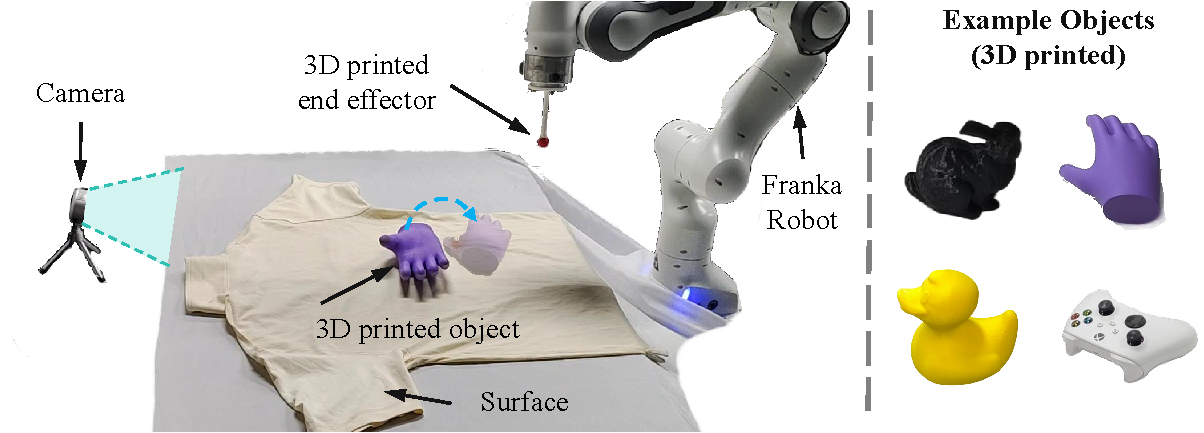
\includegraphics[width=\columnwidth]{figures/hardware_setup.pdf}}
\caption{Hardware setup of the real-world experiments.}
\label{fig:illustrative_example_1}
\end{figure}
\subsubsection{Experimental Setup}
We conduct experiments using a Franka Emika Panda equipped with a 3D-printed end-effector, and arbitrarily select 4 irregularly shaped objects: Duck, Bunny, Hand, and Xbox Controller, as shown in Fig. \ref{fig:illustrative_example_1}. We evaluate on-ground rotation on Duck and Bunny, and on-ground flipping on Bunny, Hand, and Xbox Controller. The object CAD models are obtained from the ContactDB dataset and online repositories. To validate the robustness of our method under inaccurate dynamics, we provide only rough estimates of the object’s physical parameters such as mass and friction coefficients. Moreover, instead of relying on precise motion capture for exact perception, we perform state estimation by \texttt{FoundationPose} \cite{wen2024foundationpose} using a single-view camera (Realsense D435i). In real-world experiments, precise object–environment contact locations are not directly observable. \rev{To support visualization and coarse kinematic alignment, we maintain a MuJoCo proxy of the table and end-effector, as shown in Fig. \ref{fig:illustrative_example_i}. We calibrate only the object scale and positional offsets $[\Delta x, \Delta y, \Delta z]$ from kinesthetic teaching. The proxy is not used as a physical object-contact model: the rendered object pose is updated in real time from \texttt{FoundationPose}, and no object collision geometry is defined in the simulator.} The goal pose range, success conditions, and maximum execution steps for the task are identical to those in the simulation experiments. Sampling and DyWA use the same settings as in the previous section, and the outputs of DyWA are executed using an impedance controller.
\begin{figure}[!t]
 \centerline{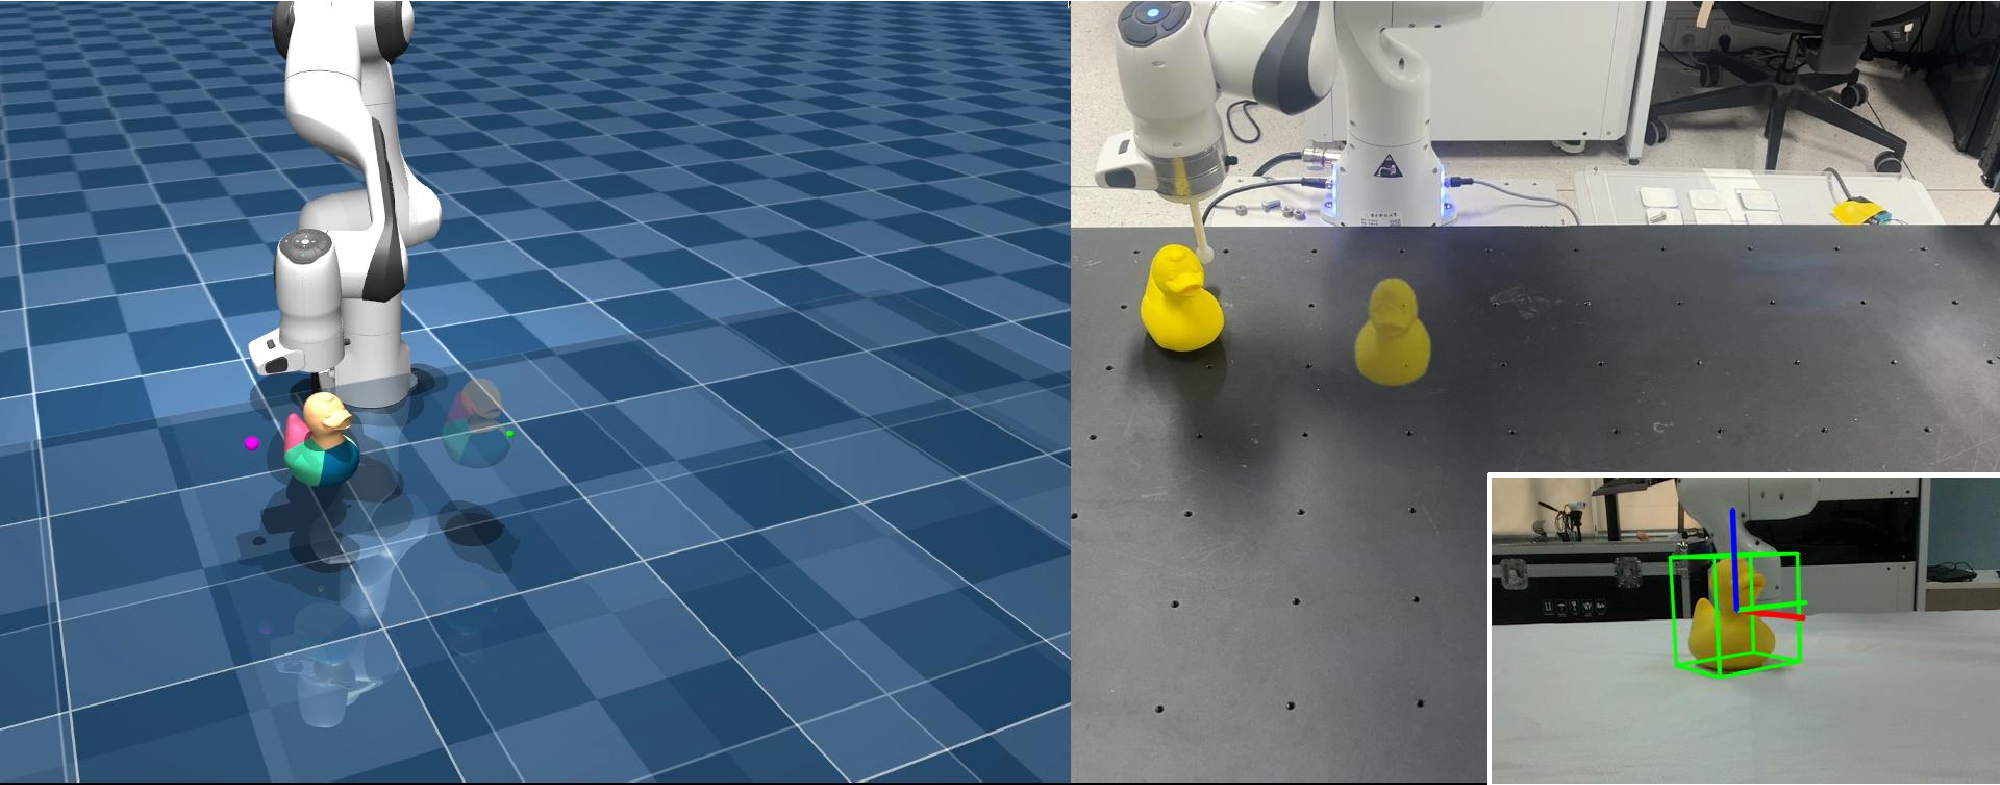
\includegraphics[width=\columnwidth]{figures/contact_sim.pdf}}
\caption{Perception method in the real-world experimental setting. Object pose is detected using \texttt{FoundationPose} and filtered via a Kalman filter. Contact estimation is performed using a \texttt{MuJoCo} implementation that approximates the experimental environment.}
\label{fig:illustrative_example_i}
\end{figure}

\begin{figure*}
 \centerline{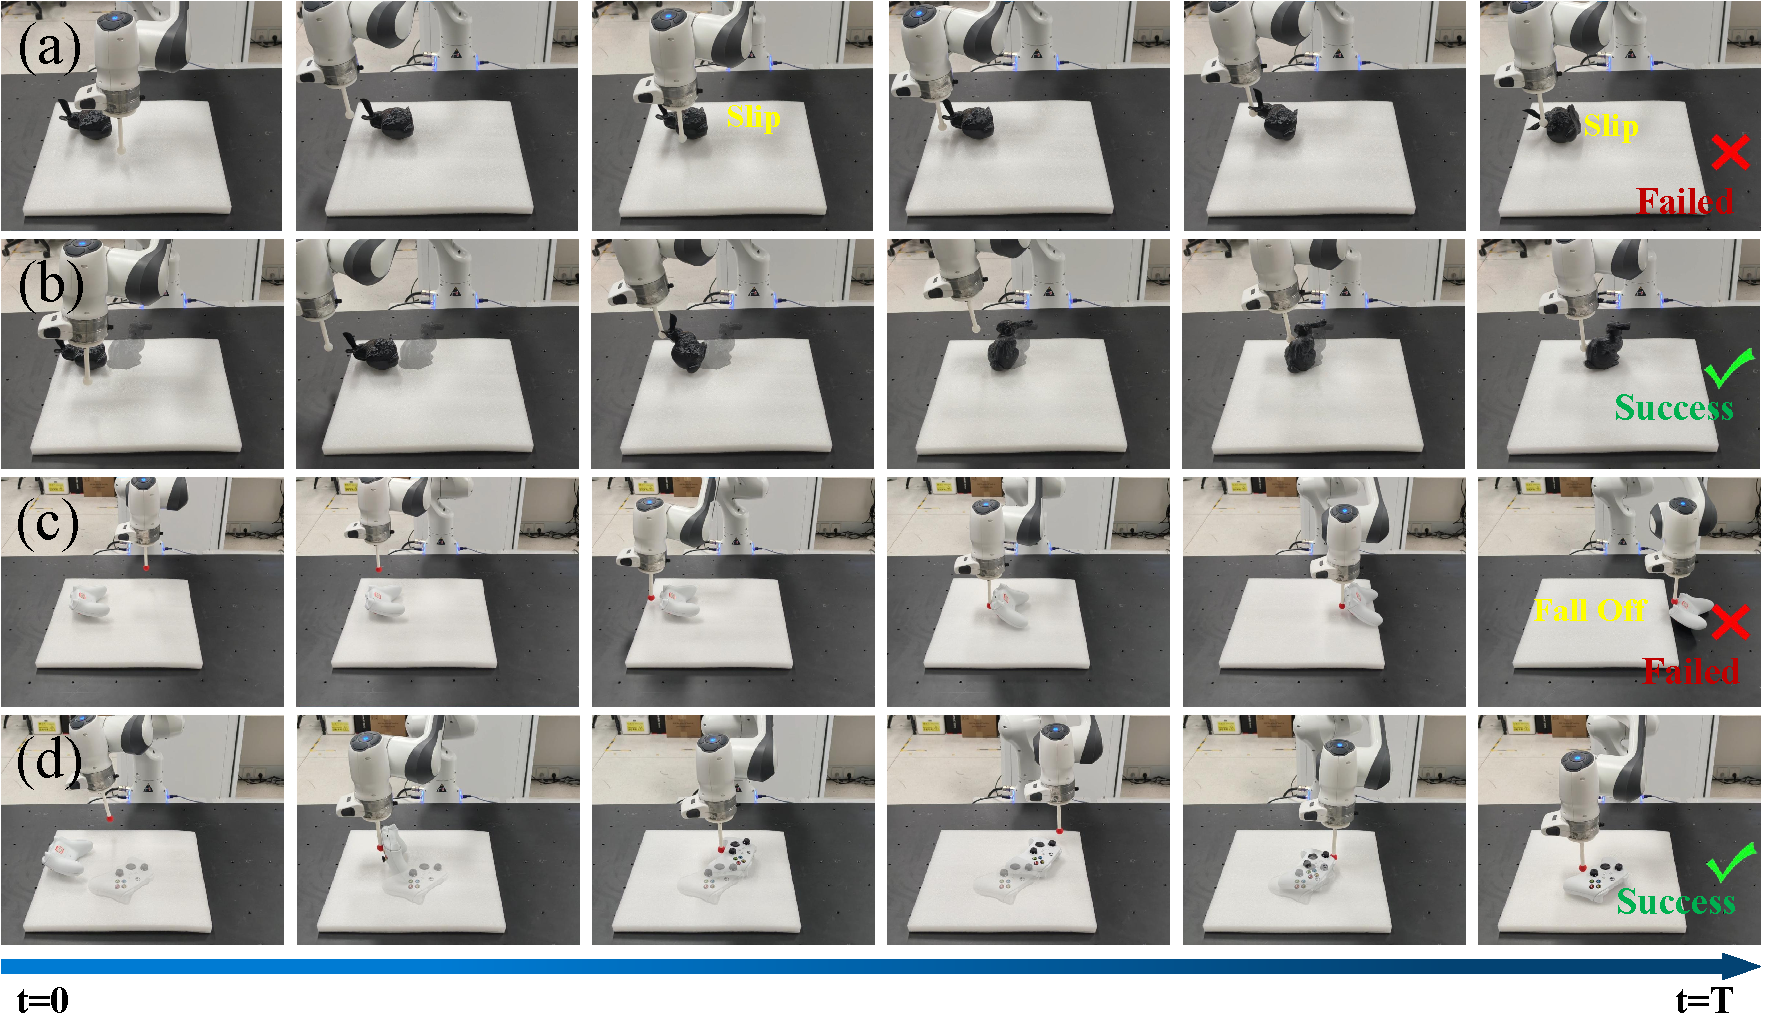
\includegraphics[width=0.9\textwidth]{figures/real_world_exps.pdf}}
\caption{Snapshots of nonprehensile manipulation in real-world experiments. (a) \textbf{DyWA} failed to flip the bunny. (b) \textbf{SCSP} succeeds in flipping the bunny. (c) \textbf{Sampling} failed by pushing the Xbox controller to fall off the foam padding. (d) \textbf{SCSP} succeeds in flipping the Xbox controller.}\label{fig:results_real_world_flip}
\end{figure*}
The OSC controller is implemented in \textsf{c++}. Unlike in simulation experiments, control in real-world deployment is subject to disturbances, leading to control lag and steady-state errors. To address this, we designed an adaptive controller for precise control, which we refer to as the Incremental OSC. We introduce an intermediate position vector $\boldsymbol{p}_{\text{inc}} = \boldsymbol{p}_{\text{inc}} + \boldsymbol{K}_{\text{inc}}\boldsymbol{u}$,
and replace $\boldsymbol{e}_{\text{pos}}$ with $\boldsymbol{e}_{\text{pos}}=\boldsymbol{p}_{\text{inc}}-\boldsymbol{p}_{\text{ee}}$. The steady-state error is adaptively eliminated under the high-frequency self-integrating effect. In the experiment, we set
$\boldsymbol{K}_{\text{inc}}=0.01 \boldsymbol{I}_3$, $\boldsymbol{K}_x = \text{diag}(500,500,500,10,10,10)$ and $\boldsymbol{D}_x = \sqrt{2\boldsymbol{K}_x}$.

\subsubsection{Results and Discussion}

\rev{We first evaluate the success rate of SCSP across different objects and tabletop materials to assess its robustness under model inaccuracies. The experimental results are shown in Fig. \ref{fig:results_real_world_flip}, \ref{fig:real_world_continous}, and Table~\ref{tab:real_world_success}. They indicate that our method maintains strong performance under perception noise and model mismatch.}
In Table~\ref{tab:real_world_success}, the 95\% CI rows report two-sided Wilson confidence intervals for SR. Bold denotes the highest SR or the lowest FR, TR, and mean ET under the same condition.

\begin{table*}[t]
\centering
\caption{Real-world manipulation performance on smooth and rough surfaces (30 trials per condition).}
\label{tab:real_world_success}
\setlength{\tabcolsep}{2.5pt}
\renewcommand{\arraystretch}{1.1}
\scriptsize
\resizebox{\textwidth}{!}{
\begin{tabular}{@{}ll*{3}{c}|*{3}{c}|*{3}{c}|*{3}{c}|*{3}{c}@{}}
\hline
\multirow{3}{*}{\textbf{Surface}} & \multirow{3}{*}{\textbf{Metric}}
& \multicolumn{6}{c|}{\textbf{Rotation}} & \multicolumn{9}{c}{\textbf{Flipping}} \\
\cline{3-17}
& & \multicolumn{3}{c|}{\textbf{Duck}} & \multicolumn{3}{c|}{\textbf{Bunny}}
& \multicolumn{3}{c|}{\textbf{Bunny}} & \multicolumn{3}{c|}{\textbf{Hand}} & \multicolumn{3}{c}{\textbf{Xbox}} \\
\cline{3-17}
& & Sampling & DyWA & \textbf{SCSP*} & Sampling & DyWA & \textbf{SCSP*} & Sampling & DyWA & \textbf{SCSP*} & Sampling & DyWA & \textbf{SCSP*} & Sampling & DyWA & \textbf{SCSP*} \\
\hline
\multirow{5}{*}{Smooth} & SR (\%) & 60 & 50 & \textbf{100} & 40 & 40 & \textbf{100} & 0 & 0 & \textbf{46.7} & 13.3 & 0 & \textbf{70} & 10 & 13.3 & \textbf{80} \\
 & FR (\%) & 6.7 & 10 & \textbf{0} & 6.7 & 10 & \textbf{0} & 20 & \textbf{0} & \textbf{0} & 23.3 & 6.7 & \textbf{0} & 16.7 & 6.7 & \textbf{0} \\
 & TR (\%) & 33.3 & 40 & \textbf{0} & 53.3 & 50 & \textbf{0} & 80 & 100 & \textbf{53.3} & 63.3 & 93.3 & \textbf{30} & 73.3 & 80 & \textbf{20} \\
 & 95\% CI & [42.3, 75.4] & [33.2, 66.8] & [88.6, 100.0] & [24.6, 57.7] & [24.6, 57.7] & [88.6, 100.0] & [0.0, 11.4] & [0.0, 11.4] & [30.2, 63.9] & [5.3, 29.7] & [0.0, 11.4] & [52.1, 83.3] & [3.5, 25.6] & [5.3, 29.7] & [62.7, 90.5] \\
 & ET (s) & 15.31 \textpm{} 10.17 & \textbf{15.19 \textpm{} 10.31} & 18.21 \textpm{} 6.42 & 17.12 \textpm{} 8.83 & 17.21 \textpm{} 8.22 & \textbf{14.57 \textpm{} 5.69} & -- & -- & \textbf{22.34 \textpm{} 12.41} & 25.90 \textpm{} 10.87 & -- & \textbf{20.19 \textpm{} 11.59} & 19.86 \textpm{} 2.15 & 27.31 \textpm{} 9.67 & \textbf{17.89 \textpm{} 10.09} \\
\hline
\multirow{5}{*}{Rough} & SR (\%) & 53.3 & 46.7 & \textbf{96.7} & 40 & 36.7 & \textbf{100} & 0 & 0 & \textbf{66.7} & 10 & 10 & \textbf{83.3} & 16.7 & 20 & \textbf{83.3} \\
 & FR (\%) & 6.7 & 13.3 & \textbf{0} & 3.3 & 6.7 & \textbf{0} & 10 & 20 & \textbf{0} & 20 & 10 & \textbf{0} & 16.7 & 16.7 & \textbf{0} \\
 & TR (\%) & 40 & 40 & \textbf{3.3} & 56.7 & 56.7 & \textbf{0} & 90 & 80 & \textbf{33.3} & 70 & 80 & \textbf{16.7} & 66.7 & 63.3 & \textbf{16.7} \\
 & 95\% CI & [36.1, 69.8] & [30.2, 63.9] & [83.3, 99.4] & [24.6, 57.7] & [21.9, 54.5] & [88.6, 100.0] & [0.0, 11.4] & [0.0, 11.4] & [48.8, 80.8] & [3.5, 25.6] & [3.5, 25.6] & [66.4, 92.7] & [7.3, 33.6] & [9.5, 37.3] & [66.4, 92.7] \\
 & ET (s) & 18.08 \textpm{} 8.01 & \textbf{16.88 \textpm{} 8.90} & 19.25 \textpm{} 9.58 & 18.41 \textpm{} 6.73 & 25.25 \textpm{} 10.05 & \textbf{15.56 \textpm{} 7.81} & -- & -- & \textbf{21.21 \textpm{} 9.97} & 26.61 \textpm{} 11.32 & 27.99 \textpm{} 9.73 & \textbf{20.30 \textpm{} 5.83} & 18.90 \textpm{} 13.26 & 21.08 \textpm{} 11.35 & \textbf{18.39 \textpm{} 11.86} \\
\hline
\end{tabular}
}
\par\smallskip
\parbox{\textwidth}{\scriptsize SR: success rate; FR: fall-out rate; TR: timeout rate; ET: execution time.}
\end{table*}

\begin{table}[t]
\centering
\caption{Failure case analysis in real-world experiments.}
\label{tab:scsp_real_world_events}
\setlength{\tabcolsep}{3pt}
\renewcommand{\arraystretch}{1.05}
\scriptsize
\resizebox{\columnwidth}{!}{
\begin{tabular}{l*{5}{c}*{5}{c}}
\toprule
\multirow{2}{*}{\textbf{Metric}}
& \multicolumn{5}{c}{\textbf{Trials}}
& \multicolumn{5}{c}{\textbf{Recovery Rate}} \\
\cmidrule(lr){2-6}\cmidrule(lr){7-11}
& Sampling & DyWA & \textbf{SCSP} & \rev{A8} & \rev{A9}
& Sampling & DyWA & \textbf{SCSP} & \rev{A8} & \rev{A9} \\
\midrule
Perception & 2/300 & 8/300 & 1/300 & 1/300 & 0/300 & 0/2 & 0/8 & 0/1 & 0/1 & -- \\
Contact Estimation & 300/300 & 300/300 & 300/300 & 300/300 & 300/300 & 73/300 & 65/300 & 248/300 & 58/300 & 37/300 \\
Slippage & 110/300 & 147/300 & 108/300 & 158/300 & 142/300 & 20/110 & 20/147 & 98/108 & 26/158 & 19/142 \\
Control Saturation & 8/300 & 45/300 & 27/300 & 85/300 & 11/300 & 2/8 & 7/45 & 25/27 & 32/85 & 10/11 \\
Poor Contact Selection & 62/300 & 15/300 & 15/300 & 90/300 & 14/300 & 12/62 & 3/15 & 3/15 & 0/90 & 0/14 \\
\rev{Contact Switching} & NR & NR & NR & NR & NR & NR & NR & NR & NR & NR \\
\bottomrule
\end{tabular}
}
\end{table}

We conducted each experiment on two different tabletop materials: smooth and rough as in Fig. \ref{fig:real_world_disturbance}. For the on-ground rotation experiments, the smooth surface denotes a tabletop with low friction, whereas the rough surface denotes cotton clothes. For the on-ground flipping experiments, which require greater friction, we use foam padding as the rough surface and cotton cloth as the smooth surface. Note that our method does not measure friction coefficients, object mass, or other physical parameters, but instead uses coarse estimates. Additionally, biases in contact estimation and noise in object pose estimation can interfere with the decision-making of SCSP. The experiment results suggest that SCSP can effectively cope with model inaccuracies and disturbances, which is typically challenging for model-based methods.

As shown in Table~\ref{tab:real_world_success}, SCSP achieved a 99.2\% success rate (119/120) in the on-ground rotation experiments with complex object geometries and also showed strong performance in the flipping tasks, whereas the comparison methods failed in nearly all flipping experiments. \rev{The execution times indicate that SCSP also completes the tasks relatively efficiently, with mean times of approximately 15--30~s across the tested conditions. } \textcolor{red}{SCSP has the highest estimated success rate under every condition, and its 95\% Wilson interval does not overlap with that of either comparison method in any condition. We report these intervals as uncertainty estimates for each success rate rather than as a formal hypothesis test between methods.} \rev{ We also classify all unsuccessful trials by their terminal outcomes: timeout or falling off the table. Most unsuccessful trials terminate due to timeout.}

\rev{We further examine five factors associated with task failures: perception failure, contact estimation error, slippage, control saturation, and poor contact selection. Perception failure denotes target tracking loss in \texttt{FoundationPose} with an unrecoverable pose estimate. It is rare and occurs only under severe occlusion when the robot reaches to retrieve an object near the table edge. Contact estimation error includes missed physical contact and reported penetration before actual contact. Slippage denotes unstable robot--object contact with relative sliding. It particularly affects flipping, where complex object geometry and smooth 3D-printed surfaces can prevent stable fingertip contact and compromise the planned motion. Surface friction also influences flipping performance, with SCSP achieving higher success rates on the rough surface. Control saturation occurs when adaptive-controller overshoot produces excessive contact commands that reach the robot's control limits and may topple the object. Poor contact selection is defined as selecting the same contact location again after three consecutive unsuccessful manipulation attempts at that location. We record the occurrence frequencies and task success rates among affected trials for SCSP, DyWA, Sampling, A8, and A9. Table~\ref{tab:scsp_real_world_events} summarizes the occurrence frequencies and recovery rates. DyWA failures mainly involve contact slippage and violations of the Franka acceleration limits during pressing. Sampling failures involve unstable contact locations.}

\rev{Contact estimation errors can falsely indicate penetration or miss existing physical contact. SCM sets $\phi\equiv0$ to suppress spurious repulsive wrenches induced by estimated penetration, while CPO attracts the end-effector toward an inward-offset target rather than the estimated surface, helping avoid local minima above the physical surface. We compare A8, which removes the $\phi\equiv0$ condition, and A9, which replaces the target in \eqref{eq:placing_cost} with the surface point $\boldsymbol{p}_{\text{ref}}$. Table~\ref{tab:scsp_real_world_events} summarizes the comparison. A9 sometimes stalls above the object without establishing contact, leading to timeout. A8 is particularly sensitive to contact estimation errors: when \texttt{FoundationPose} estimates an object pose penetrating the ground, we observe abrupt changes in A8's predicted object positions, sometimes causing premature contact loss during flipping and subsequent object toppling.}

We further conduct continuous manipulation experiments, as shown in Fig. \ref{fig:real_world_continous}. During manipulation, we repeatedly perturb the object pose to evaluate the real-time performance, closed-loop planning capability, and robustness of SCSP under accumulated perception errors. Under repeated perturbations, both the pose estimated from \texttt{FoundationPose} and the contact estimation become biased. However, SCSP exhibits strong replanning capability and consistently completes the continuous manipulation tasks under disturbances.

We combine the preceding experimental results to analyze the source of SCSP’s robustness to model mismatch. We conclude that: 1) the ablation study reveals that optimality of the contact prior is not necessary. Although the prior is important for contact planning, even a coarse contact location selection as a prior can still bring substantial performance improvement. This observation also provides insight into the role of the contact-selection model: how to properly connect the prior with the planning framework seems to be more important than the optimality and accuracy of the prior itself. The designs of CSO and the ranking strategy are both developed with this perspective. 2) CPO has a strong closed-loop nature. The real-time performance and robustness of CIMPC methods have been thoroughly validated in previous work. CPO is a prior-guided contact planning framework built upon the CIMPC formulation. It inherits the robustness of CIMPC while improving manipulation diversity. Therefore, the SCSP framework is able to achieve robust performance.

\begin{table}[t]
\centering
\caption{Computation time of SCSP}
\label{tab:metrics}
\begin{tabular*}{0.8\columnwidth}{@{\extracolsep{\fill}} l c}
\toprule
\textbf{Metric} & \textbf{Value} \\
\midrule
\textcolor{red}{Offline sampling cost time} (s) & 4.82$\pm$3.85 \\
Exchange cost time (ms) & 0.002$\pm$0.01 \\
CSO solving time (ms) & \rev{2.35$\pm$0.73} \\
RS cost time (ms) & 5.99$\pm$2.76 \\
Average CPO solving time (ms) & 8.68$\pm$0.31 \\
\bottomrule
\end{tabular*}
\end{table}

\begin{figure*}
 \centerline{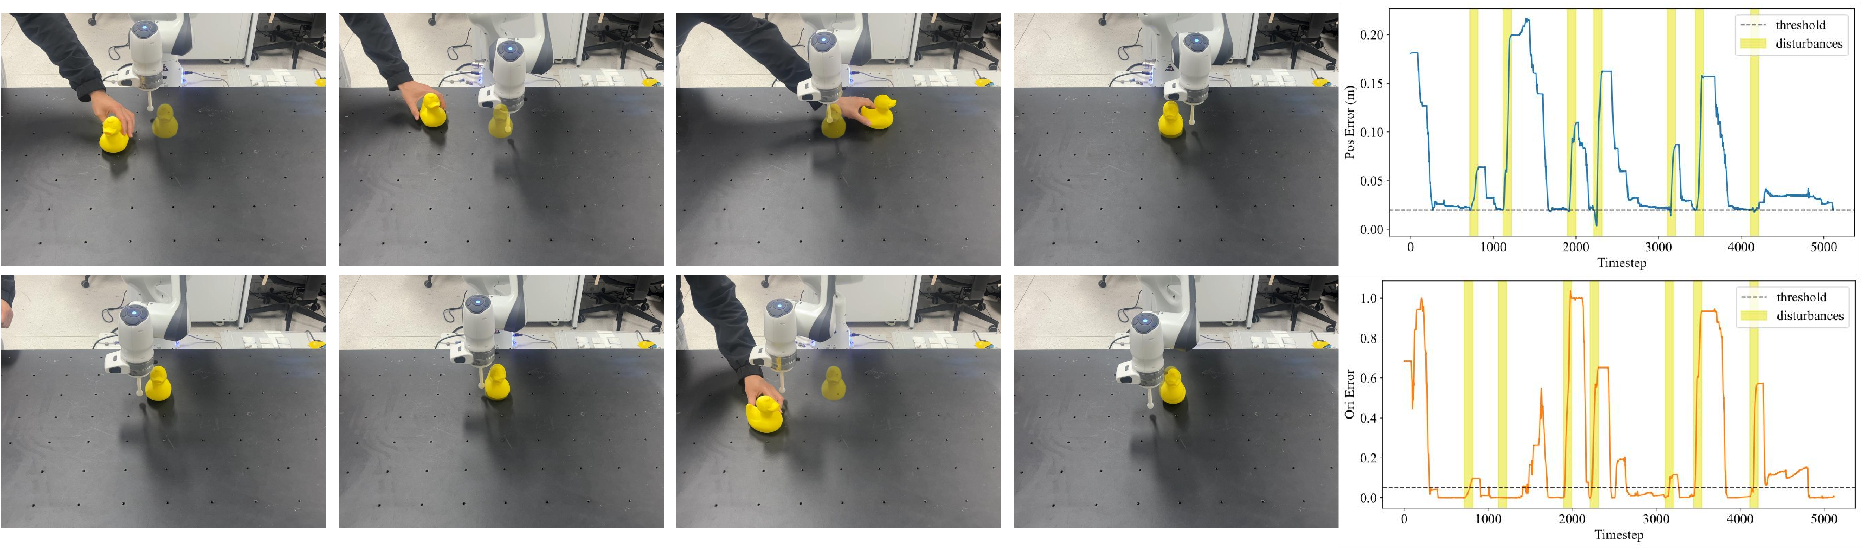
\includegraphics[width=0.9\textwidth]{figures/consecutive_manipulation.pdf}}
\caption{Snapshots of manipulation under external disturbances. The object’s pose is continuously perturbed during manipulation to demonstrate SCSP’s real-time robustness under such disturbances. The panels on the right show the temporal evolution of position and orientation errors.}\label{fig:real_world_continous}
\end{figure*}

\begin{figure}
 \centerline{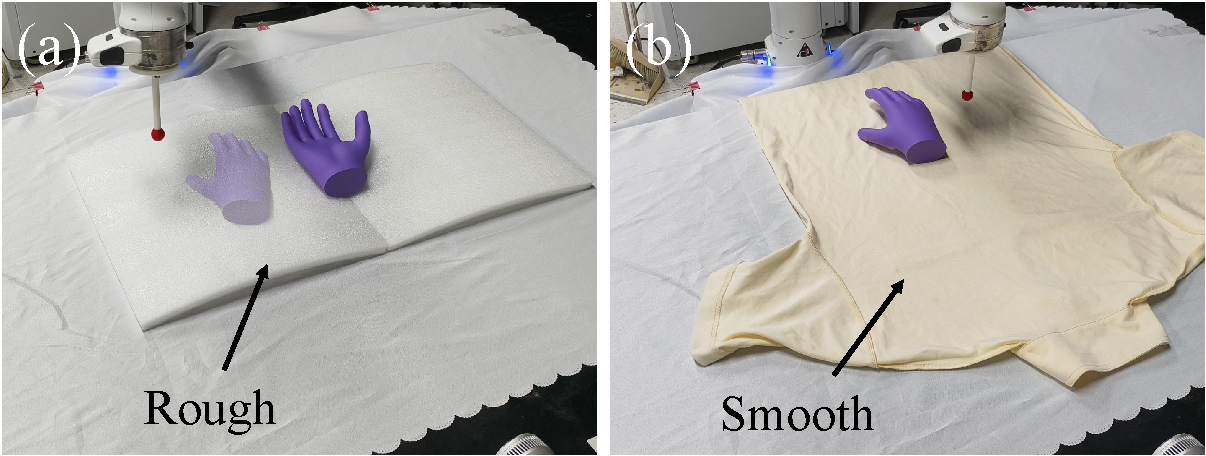
\includegraphics[width=\columnwidth]{figures/real_world_2.pdf}}
\caption{Robustness validation of SCSP on surfaces with different friction. (a) Foam. (b) Cotton clothes.}\label{fig:real_world_disturbance}
\end{figure}

\section{Generalization to Multiple Tasks}\label{sec:generalize}

We further implement SCSP in different scenarios to evaluate its generalization. Using multi-contact tasks and long-horizon tasks as examples, we demonstrate that SCSP can perform \rev{online contact selection} and execute more complex manipulation tasks on more underactuated objects.

\subsection{Case Study I: Multi-Contact Task}

SCSP can be easily extended to multi-contact tasks. We illustrate the generalization of SCSP with following example:
\subsubsection{Soccer Dribbling}
We use a soccer dribbling task to demonstrate \rev{the performance of SCSP in dynamic scenarios}. In this task, SCSP plans contact with the ball using one of the two feet and drives it toward the goal through multi-contact manipulation. The main challenges lie in the highly dynamic behavior of the ball, which makes stable and sustained contact difficult, and in coordinating the two feet effectively. We read the ball position $\boldsymbol{p}_k$ and estimate its velocity $\boldsymbol{v}_k$ from the simulation using a Kalman filter. The 3D model of the ball is then input to the SCSP to compute the actions $\boldsymbol{u} \in \mathbb{R}^{2\times 4}$ for both feet, where the control vector for each foot is $\left [ x,y,z,\theta_{\mathrm{yaw}} \right ] $. We define activation triggers separately for the left and right feet: using the midpoint between both feet as the center, the space is divided into left and right half-spaces. When $\boldsymbol{x}_k$ appears in a half-space, the corresponding left or right foot is activated. Additionally, workspace constraints (represented as semi-transparent cubes) are imposed on each foot to prevent singular gait patterns. The number of CSO sampling points is set to $n_s=70$, and points close to the ground $\left \{ p_i\in\mathcal{I}_{\text{obj}} \ | \ z_i < 0.02\mathrm{m}  \right \}$ are masked out. We randomly selected 10 goal positions for the soccer ball, and SCSP continuously controlled the robot’s feet to dribble the ball to each target, achieving a 100\% success rate. The experimental results are shown in Fig. \ref{fig:soccer}. This experiment serves as a toy example, simulating the approaching and contact phases in humanoid soccer dribbling. In the future, we plan to extend SCSP to more complex motion planners to realize a more complete demonstration \cite{yin2025visualmimic, kong2026learning}.
\begin{figure}[!t]
 \centerline{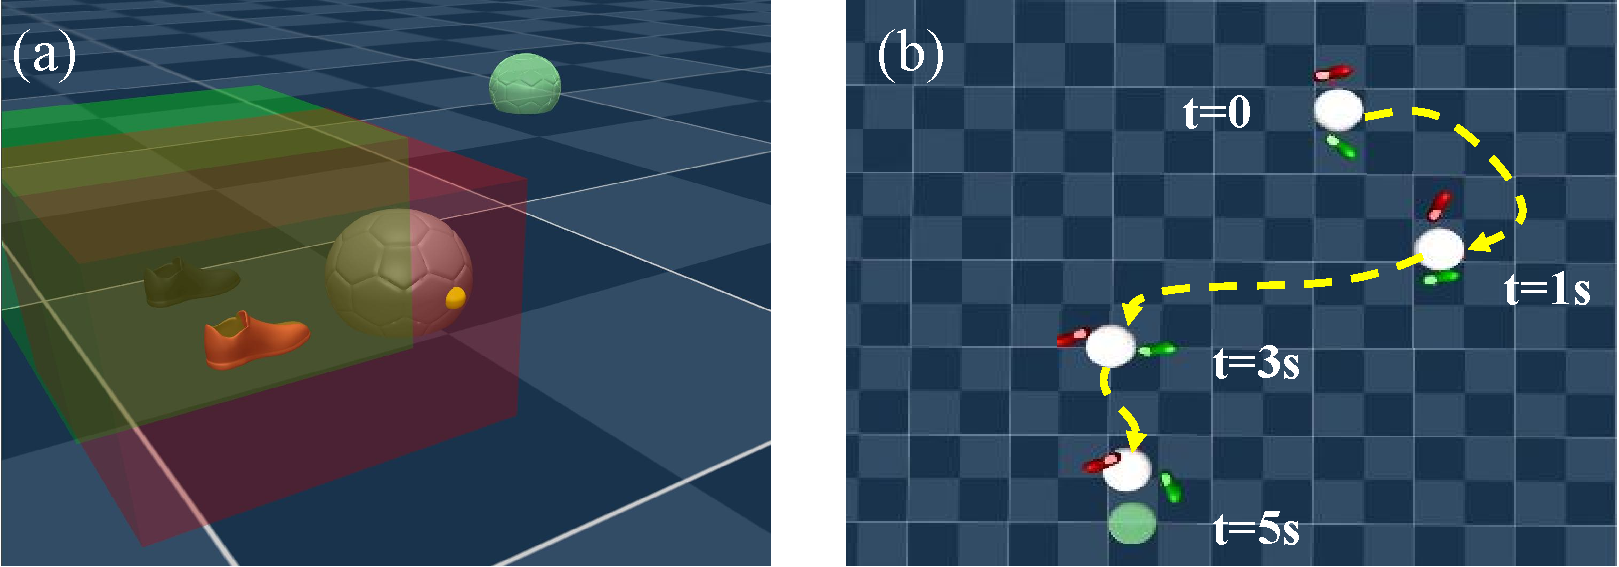
\includegraphics[width=\columnwidth]{figures/soccer2.pdf}}
\caption{Soccer dribbling task. (a) Experiment setup. The task is to kick the soccer to the target (translucent). Red and green cubes show footworkspaces, and the yellow point indicates CSO-planned contact locations. (b) Gribbling trajectory.}
\label{fig:soccer}
\end{figure}
\subsubsection{Tilted Pushing} 

SCSP can be extended to manipulation tasks in uneven environments, such as tilted pushing. Stable object poses on a slope are inherently fragile, requiring accurate contact location selection and online replanning. We compare open-loop methods, which plan a contact sequence offline, with SCSP, which replans online during execution. As the baseline, we use STOCS-3D to compute an offline sequence of contact locations and contact forces, and execute this sequence using our CPO. Experiments are conducted in \texttt{IsaacGym} with a 15$^\circ$ slope and a friction coefficient of 0.1. For SCSP, we set $w_{\text{stab}}=0$ and $\hat{\lambda}^n_{\text{max}}=0.5$, while keeping all other parameters the same as in Section~\ref{sec:robot_manipulation}. We selected the teapot and duck (used in previous experiments) and randomly set 10 stable poses on the slope as goal poses, and pushed and rotated the objects from below to reach these goals. The results in Table~\ref{tab:generalization_tasks_result} and Fig.~\ref{fig:tilted_push} show that the real-time replanning capability of SCSP provides substantially better robustness.

\begin{figure}[!t]
 \centerline{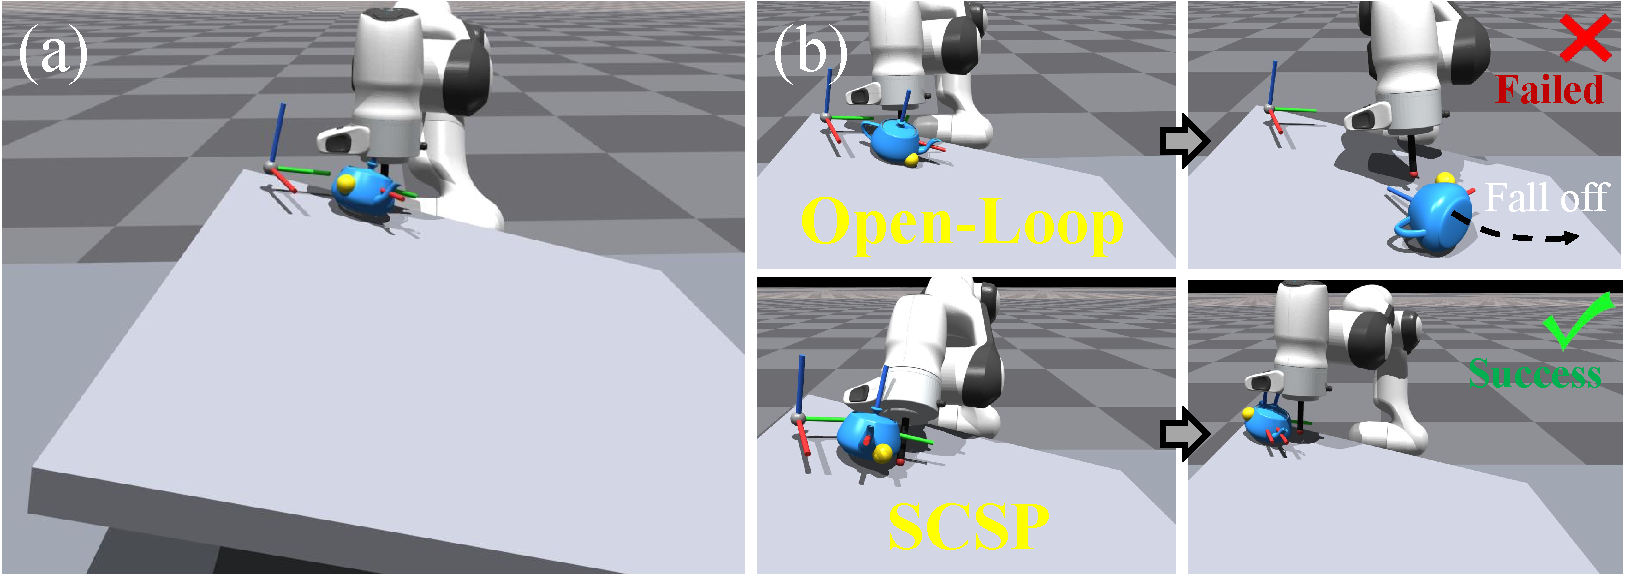
\includegraphics[width=\columnwidth]{figures/tilted_pushing.pdf}}
\caption{Experiment setup. The task is to push an object on a surface tilted at 15$^\circ$. (a) The open-loop method fails when execution errors occur, causing the teapot to fall off the tilted surface. (b) SCSP can replan online and thus successfully complete the dynamic task.}\label{fig:tilted_push}
\end{figure}
\subsubsection{Grasping \& Dexterous Manipulation} 
SCSP can also be applied to predict grasping poses, such as bimanual grasping and multi-finger grasping. Following \cite{lin2026bidexgrasp}, we use the Grasp Wrench Boundary (GWB) \cite{borst2004grasp} to select grasping regions and identify the top-K pairs of potential valid regions for grasping. Subsequently, sampling of the candidate set $\mathcal{I}_{\text{obj}}$ is performed within these regions. The objective of the CSO inner loop optimization is then transformed to force closure:
\begin{equation}\label{equ:force_closure}
    \begin{aligned}
\min_{\boldsymbol{\hat{\lambda}}_r \in \mathcal{K}}
\quad &
\sum_{j=1}^{N_d} \left\| \xi \boldsymbol{w}^{(j)} - \boldsymbol{J}_o \boldsymbol{\hat{\lambda}}_r^{(j)} \right\|_2^2
\;+\;
w_{\lambda} \sum_{j=1}^{n_d} \left\| \boldsymbol{\hat{\lambda}}_r^{(j)} \right\|_2^2 \\
\text{s.t.}\quad
& \sum_{i=1}^{K} \hat{\lambda}_r^{(j),n} \ge \zeta, \ 
\forall j=1,\dots,n_d .
\end{aligned}
\end{equation}
where $n_c$ is the number of robot contact points, $n_d$ denotes the number of sampled disturbance wrenches, $\boldsymbol{w}^{(j)} \in \mathbb{R}^6$ represents the $j$-th disturbance wrench. $\boldsymbol{\lambda}_r^{(j)}$ denotes the robot contact force corresponding to disturbance $\boldsymbol{w}^{(j)}$. $\xi$ is the disturbance scaling factor, $\zeta$ the minimum total normal force required to maintain an active grasp and $w_{\lambda}=0.1$. During each rollout, the CSO in SCSP solves \eqref{equ:force_closure} for the nearest points $\boldsymbol{p}_{\text{near}}^i$ to the robot end-effector or Allegro fingers additional to the top 5 pairs of potential grasping pairs, thereby searching for grasping poses online. We use an open-loop baseline that computes the optimal grasping locations offline using CSO and executes them online with CPO for comparison. For bi-manual and multi-finger grasping, we selected five objects each, placed them on a pedestal (black), randomly perturbed their yaw angles $\theta_{\text{yaw}}$ and scaled their sizes by a random factor $\varsigma \in \left \{ 0.5,1,1.5,2 \right \} $, conducting 20 trials for each task. The results are shown in Table~\ref{tab:generalization_tasks_result} and Fig.~\ref{fig:grasping}. SCSP achieves a higher success rate than the baseline in these trials; however, it fails on some objects with complex geometry because convexification of the collision mesh by \texttt{MuJoCo}.
\begin{figure}[!t]
 \centerline{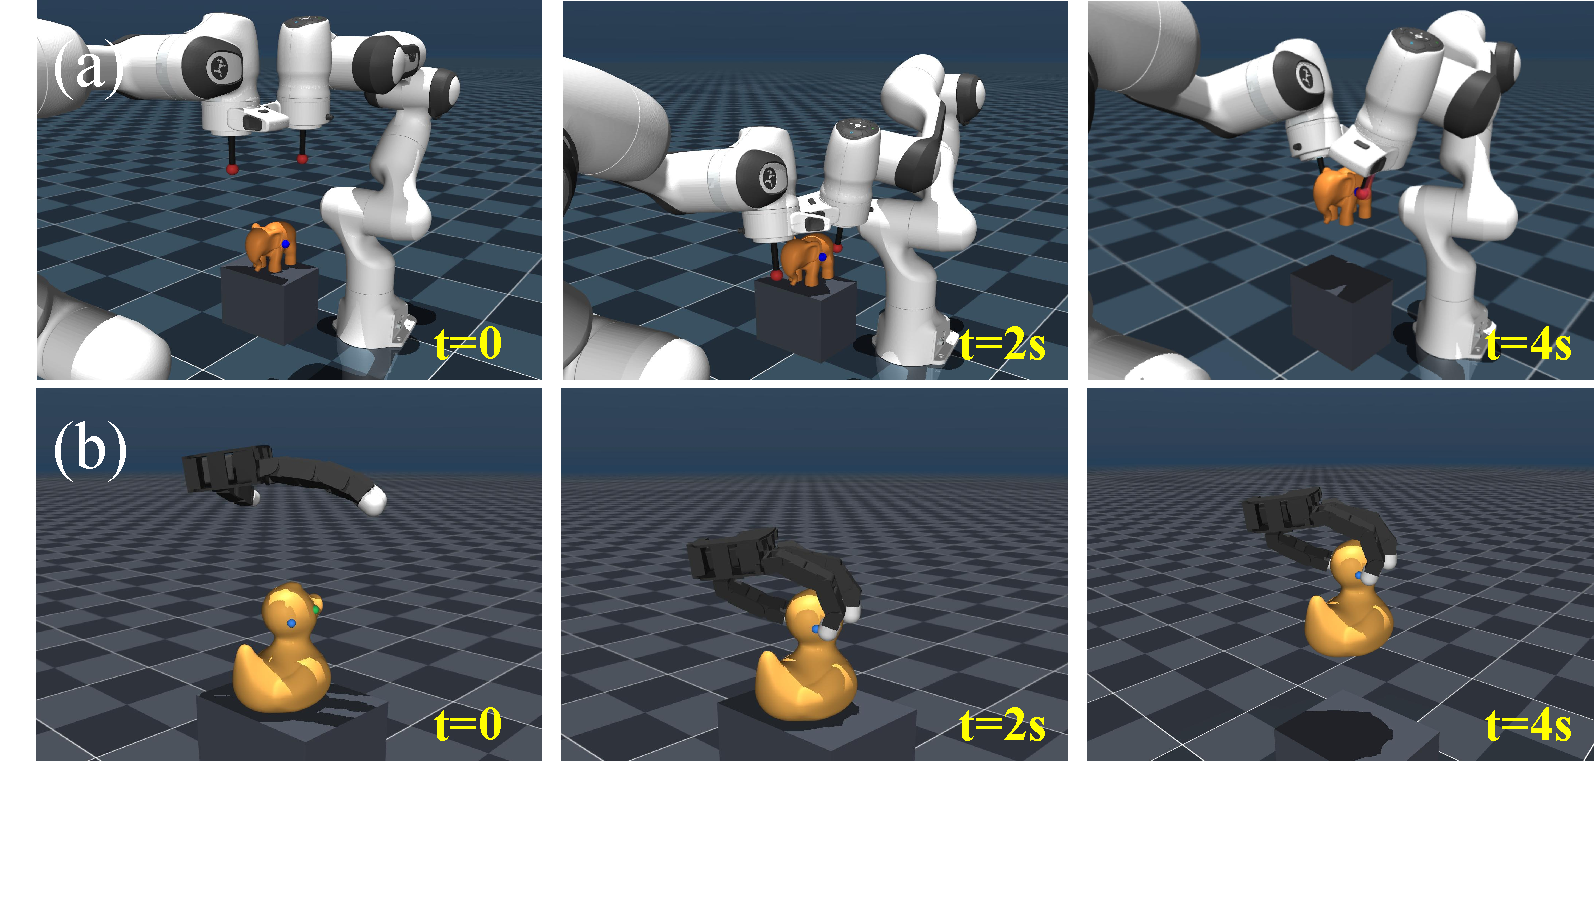
\includegraphics[width=\columnwidth]{figures/grasping.pdf}}
\caption{Snapshots of the multi-contact grasping tasks. (a) Bi-manual grasping of an elephant with the size scaling factor $\varsigma=1$. (b) Multi-finger grasping of a duck with $\varsigma=1.5$.}
\label{fig:grasping}
\end{figure}
\subsection{Case Study II: Articulated Object Manipulation}
\rev{SCSP uses active contact selection to perform articulated object manipulation. We evaluate this capability on a drawer and a microwave door, which require sequential contact interactions.} The tasks are to pull the drawer to a target displacement and to open the microwave door to a target angle. In both tasks, the object is semantically segmented into different parts, such as handles, while non-manipulable parts are excluded. For the drawer, we directly compute the final pulled-out pose as the goal pose. For the microwave, which involves rotational motion, we set the goal pose of each rollout as the \texttt{SLERP} interpolation between the current state and the desired door state. The parameter and cost settings of SCSP are the same as those in Section~\ref{sec:robot_manipulation}, with $w_{\text{stab}}=0$. The solver for CPO is an MPPI-based motion planner~\cite{bhardwaj2022storm}. As a baseline, we use an open-loop method that plans the contact sequence offline using CSO and executes it online with CPO, in order to demonstrate the effectiveness of online contact selection. We randomly perturbed the distance and yaw angle between the drawer or microwave and the Franka base by $\Delta d \in \left [ -0.1, 0.1 \right ] \mathrm{m}$ and $\Delta \theta_{\text{yaw}} \in \left [ -\frac{\pi}{4} , \frac{\pi}{4}  \right ]$ and conducted 10 trials for each object. The experimental results are shown in Fig.~\ref{fig:long_horizon}, Table~\ref{tab:generalization_tasks_result} and the \href{https://sites.google.com/view/scsp-robot}{website} videos. Although the success rates are comparable, the open-loop method cannot handle certain execution errors, such as contact slippage or the robot approaching singular configurations.
\begin{figure}[!t]
 \centerline{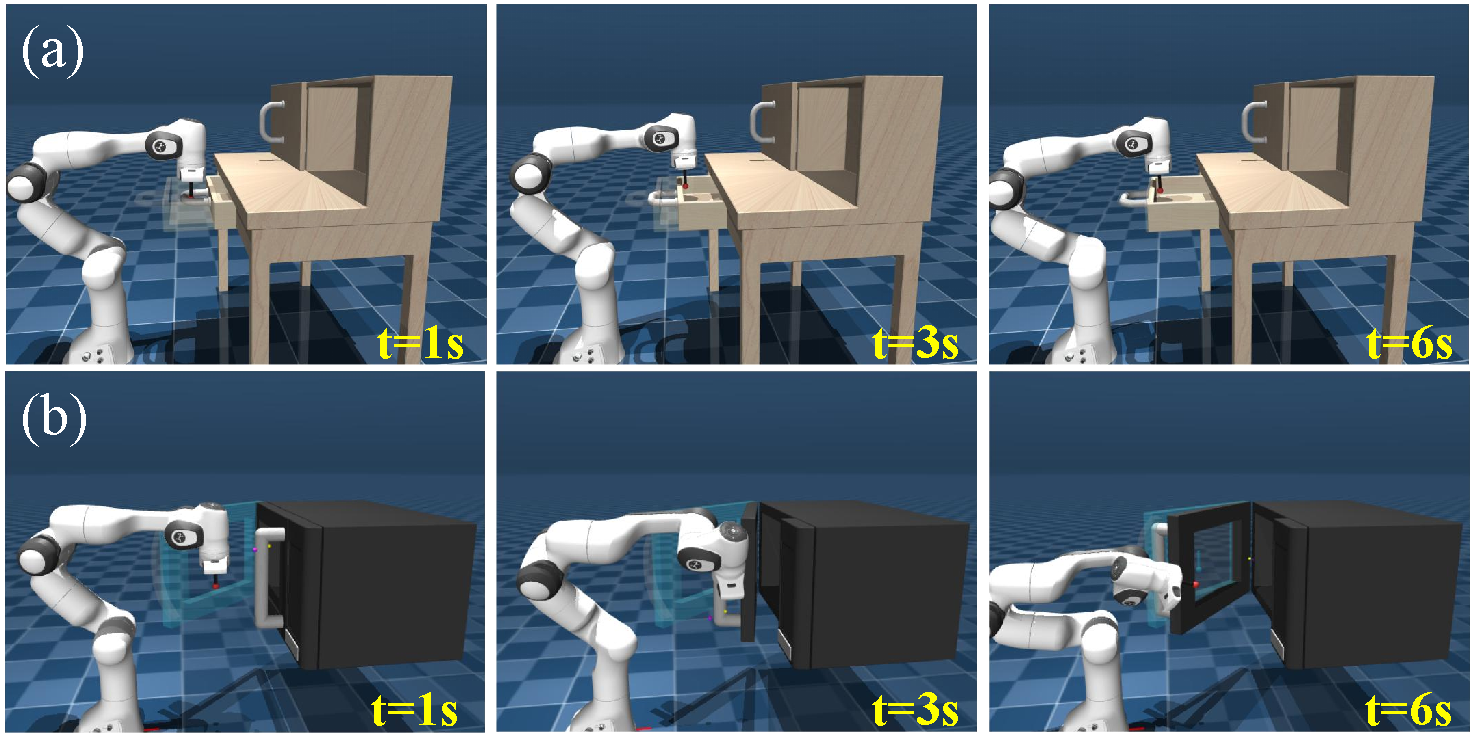
\includegraphics[width=\columnwidth]{figures/long-horizon.pdf}}
\caption{Snapshots of long-horizon tasks. Given only the target pose of the object, SCSP performs online reasoning and selects appropriate contact locations to accomplish the task. (a) Opening a drawer. (b) Opening the microwave door.}
\label{fig:long_horizon}
\end{figure}

\begin{table*}[t]
\centering
\caption{Success trials across different tasks.}
\label{tab:generalization_tasks_result}
\setlength{\tabcolsep}{5pt}
\begin{tabular*}{\textwidth}{@{\extracolsep{\fill}} lcccccccccc}
\toprule
\textbf{Metric}
& \multicolumn{2}{c}{\textbf{Soccer Dribbling}}
& \multicolumn{2}{c}{\textbf{Tilted Pushing}}
& \multicolumn{2}{c}{\textbf{Bi-Manual Grasping}}
& \multicolumn{2}{c}{\textbf{Multi-finger Grasping}}
& \multicolumn{2}{c}{\textbf{Long-horizon Tasks}} \\
\cmidrule(lr){2-3}
\cmidrule(lr){4-5}
\cmidrule(lr){6-7}
\cmidrule(lr){8-9}
\cmidrule(lr){10-11}
& \textbf{Open-Loop}
& \textbf{SCSP}
& \textbf{Open-Loop}
& \textbf{SCSP}
& \textbf{Open-Loop}
& \textbf{SCSP}
& \textbf{Open-Loop}
& \textbf{SCSP}
& \textbf{Open-Loop}
& \textbf{SCSP} \\
\midrule
\textbf{Success Trials}
& /
& \textbf{10/10}
& 0/20
& \textbf{18/20}
& 0/20
& \textbf{15/20}
& 15/20
& \textbf{16/20}
& 15/20
& \textbf{20/20} \\
\bottomrule
\end{tabular*}
\end{table*}




\section{Discussion \& Limitations}
\label{sec:discussion}

\rev{The theoretical and experimental results support the usefulness of explicit contact selection, while also exposing several limitations of the current implementation.}
\rev{CSO provides contact-location priors through mesh discretization and a lightweight surrogate contact model. This design is computationally efficient, but its accuracy decreases in complex contact configurations because it assumes a fixed object--environment contact set, restores inter-contact coupling only through three unrolled Gauss--Seidel sweeps, and represents contacts as points. CSO therefore does not provide sequential, high-fidelity state prediction and is not directly suited to complex end-effectors or deformable objects. Higher-fidelity contact models such as \cite{huang2026pointworld} are a potential direction for these capabilities, although their interfaces and task domains differ from SCM and they are not drop-in replacements.} \madd{General multi-contact manipulation remains limited by scalability: selecting $n_{\text{r}}$ robot contacts from $n_s$ candidates grows combinatorially, e.g., $\binom{n_s}{n_{\text{r}}}$ in the unordered case, and tasks with strong geometric coupling among contacts, such as power grasping, are beyond the demonstrated precision-grasping case. Reducing the CSO search space, as done with the GWB-based regions in Section~\ref{sec:generalize}, is a first step toward this direction and is left for future work.}

\rev{CPO generates trajectories for contact-free and contact-rich stages using model-predictive control. Its implementation may be less suitable for tasks such as loco-manipulation and may not maintain continuous surface contact during contact switching. Future work can replace the rule-based ranking strategy with a learned representation and can combine CPO with a more expressive motion planner such as \cite{xu2026interprior}.}

\rev{The experiments also suggest that the interface between contact selection and trajectory optimization is important: CPO can use a nearby contact point when the lowest-cost sampled point is difficult to execute. These results do not establish surrogate accuracy beyond the evaluated tasks; robustness claims therefore apply only to tested settings.}

\section{Conclusion}
\label{sec:conclusion}

\rev{This work presented SCSP, a cascaded framework that separates contact-location selection from contact-trajectory optimization for contact-rich manipulation. CSO evaluates a finite set of sampled surface points with a surrogate contact model, and CPO uses the resulting contact prior together with a ranking rule to generate approaching, contact, and contact-switching trajectories. Simulations and hardware experiments show that this decomposition can improve manipulation diversity and task success under the tested geometric and modeling conditions. The results also indicate that SCSP remains limited by the point-contact and fixed-contact-set assumptions of the surrogate model, as well as by the need for a one-time MuJoCo calibration in the vision-based hardware experiments.}


\bibliographystyle{IEEEtran}

\bibliography{reference}


\end{document}
